
\chapter[Application of The Finite Element Method To...]{Application
  of The Finite Element Method To The Approximation 
  of Some Second Order EVI}\label{chap2}%Chap II 

\section{Introduction}\label{c2:s1}%Sec 1

In\pageoriginale this chapter we consider some examples of EVI of the
first and 
second kinds. These EVI are related to second order partial
differential operators (for fourth order problems see GLOWINSKI
[\ref{k47:e2}]). The Physical Interpretation and some properties of
the solution 
are given. Finite element approximations of these EVI are considered
and convergence results are proved. In some particular cases we prove
error estimates. 

Some of the results in this chapter may be found in
G.L.T. [\ref{k53:e1}],[\ref{k53:e2}]. For the approximation of the EVI of first kind by the
finite element methods we refer also to FALK [\ref{k44:e1}], STRANG
[\ref{k84:e1}],
MOSCO-STRANG [\ref{k86:e1}], CIARLET [\ref{k31:e1}],
BREZZI-HAGER-RAVIART [1].  

We also deal with iterative methods for solving the corresponding
approximate problems (cf. CEA [\ref{k26:e1}], G.L.T. [\ref{k53:e1}],
[\ref{k53:e2}]).  

\section[An Example of EVI of The First Kind:...]{An Example of EVI of 
The First Kind: The Obstacle Problem}\label{c2:s2}%Sec 2

\begin{notations}
All the properties of Sobolev spaces used in this chapter are proved
in LIONS [\ref{k67:e2}], NECAS [\ref{k73:e1}]. Usually we shall have  
\begin{itemize}
\item $ \Omega$: a bounded domain in $\mathbb{R}^2$
\item $\Gamma: \partial \Omega$
\item $x = \{x_1, x_2\}$ a generic point of $\Omega$
\item $\nabla = \{\dfrac{\partial}{\partial x_1},
  \dfrac{\partial}{\partial x_2}\}$ 
\item $C^m (\bar{\Omega})$: space of $m$ -times continuously
  differentiable real valued functions for which all the derivatives
  up to order $m$ are continuous in $\bar{\Omega}$, 
\item $C^m_0(\bar{\Omega}) = \{v \in C^m(\bar{\Omega}): \Supp (v)
  \text{ is a compact subset of } \Omega \}$.  
\item $ \parallel  v \parallel  _{m,  p,  \Omega} = \sum\limits_{| \alpha | \leq m} \parallel 
  D^\alpha v \parallel  _{L^p(\Omega)}$\pageoriginale for $v \in
  C^{m}\overline{(\Omega)}$ where $\alpha =  (\alpha_1, \alpha_2);\break
  \alpha_1$, $\alpha_2$ non-negative integers, $|\alpha| = \alpha_1 +
  \alpha_2$ and $D^\alpha = \dfrac{\partial ^{|\alpha|}}{\partial
 x_1^{\alpha_1} \partial x^{\alpha_2}_2}$.  
\item $W^{m, p} (\Omega):$ completion of $C^m(\overline{\Omega})$ in
  the norm defined above. 
\item $W^{m, p}(\Omega)$: completion of $C^m_0 (\Omega)$ is the above
  norm 
\item $H^m (\Omega) = W^{m, 2}(\Omega)$, 
\item  $H^m_0(\Omega) =  W^{m, 2}(\Omega)$,
\end{itemize}
\end{notations}
 $\mathscr{D} (\Omega) = C^\infty_0 (\Omega)$. 
 
\subsection{The continuous problem:}\label{c2:ss2.1} 
Let  % subsec 2.1.
$$
V = H^1_0 (\Omega) = \{v \in H^1 (\Omega) : v | 
\Gamma = \text{ trace de v sur } \Gamma = 0  \} 
$$
(cf. LIONS [\ref{k67:e2}], NECAS[\ref{k73:e1}]). 
$$
a(u, v) = \int_\Omega \nabla u. \nabla v dx 
$$
where 
$$
\nabla u. \nabla v = \frac{\partial u} {\partial
  x_1} \frac{\partial v}{\partial x_1} + \frac{\partial u}{\partial
  x_2} \frac{\partial v}{\partial x_2}., 
$$
$L (v) = \langle f, v \rangle$ for $f \in V^* = H^{-1} (\Omega)$
and $v \in V$. Let $\Psi \in H^1 (\Omega) \cap C^0
(\overline{\Omega})$ and $\Psi |_\Gamma \leq 0$. Define $K = \{v
\in H^1_0 (\Omega) : v \geq \Psi a.e.$ on $\Omega \}$. 
 
Then the obstacle problem is a $(P_1)$ problem defined by :
 
\textit{Find $u$ such that}
\begin{equation}
\begin{cases}
 a(u, v-u) \geq L(v-u)\, \forall v \in K,\\
 u \in K.
\end{cases} \tag{2.1}\label{c2:eq2.1}
 \end{equation} 
 
The physical interpretation of this problem is the following: let an
elastic membrane occupy a region $\Omega$ in the $x_1$, $x_2$ plane;
this membrane is fixed along the boundary $\Gamma$ of $\Omega$. When
there is no obstacle, from the theory of elasticity the vertical
displacement $u$, obtained by applying a vertical force $F$, is given
by the Dirichlet problem 
\begin{equation}
\begin{cases}
-\Delta u = f ~~\text{\em in }~~\Omega,\\
u|_\Gamma = 0\tag{2.2}\label{c2:eq2.2}
\end{cases}
\end{equation}\pageoriginale 
 where $f = F/t$, $t$ being the tension.
 
 When there is an obstacle, we have a free boundary problem and the
 displacement $u$ satisfies the variational inequality \eqref{c2:eq2.1} with
 $\Psi$  being the height of the obstacle. Similar EVI also occur,
 sometimes with non-symmetric bilinear forms, in mathematical models
 for the following problems: 
 
 \begin{itemize}
\item Lubrication phenomena (cf. CRYER [\ref{k40:e1}]).
\item Filtration of liquids in porous media (cf. BAIOCCHI
  [\ref{k3:e1}], COMINCIOLI [\ref{k40:e1}]), 
\item Two dimensional, irrotational flows of perfect fluids
  (cf. BREZIS STAMPACCHIA [\ref{k69:e1}], BREZIS [\ref{k14:e1}],
  {\small CLAVLDINI-TOURNEMINE} [\ref{k36:e1}]).  
\item Wake problems (cf. BOURGAT- DUVAUT [\ref{k42:e1}]).
 \end{itemize} 
 
\subsection{Existence and uniqueness results:}\label{c2:ss2.2} %subsec 2.2
 
 For proving the existence and uniqueness of the problem
 \eqref{c2:eq2.1}, we 
 need the following lemmas stated below without proof (for proof of
 the lemmas, see for instance LIONS [\ref{k67:e1}], NECAS [\ref{k73:e1}],
 STAMPACCHIA [\ref{k83:e1}]).  
  
\begin{lemma}\label{c2:lem2.1}%lemma 2.1
Let $\Omega$ be a bounded domain in $\mathbb{R}^N$. Then the semi-norm
on $H^1(\Omega)$  
$$
v \to \left( \int_\Omega |\nabla _v | ^2 dx \right) ^{1/2}
$$
is a norm on $H^1_0 (\Omega)$ and it is equivalent to the norm on
$H^1_0(\Omega)$ induced from $H^1(\Omega)$. 
\end{lemma}  
  
  The above Lemma~\ref{c2:lem2.1} is known as Poincare-Friedrichs lemma.
  
\begin{lemma}[STAMPACCHIA {[\ref{k83:e1}]}]\label{c2:lem2.2}%lemma 2.2
  Let $f : \mathbb{R} \to \mathbb{R}$  be uniformly
  Lipschitz continuous  (i.e. $\exists k > 0$ such that $| f(t) -
  f(t') | \leq k | t - t'| \,\forall t$, $t' \in R)$ and such $f'$
  has a finite number of points of discontinuity. Then the induced map
  $f^*$  on $H^1(\Omega)$ defined by $u \to f (u) $ is a continuous
  map into $H^1(\Omega)$. Similar results holds for $H^1_0 (\Omega)$
  when ever $f (0) = 0$. 
  \end{lemma} 
  
\begin{corollary}\label{c2:cor2.1}%corollary 2.1
If $v^+$\pageoriginale  and $v^-$ denote the positive and the negative parts of $v$
for $v \in H^1 (\Omega)$ (respectively $H^1_0(\Omega))$ then the
map $v \to \{v^+, v^- \}$ is continuous from $H^1 (\Omega) \to H^1
(\Omega ) \times H^1(\Omega) $ (respectively $H^1_0  (\Omega) \to
H^1_0 (\Omega) \times H^1_0 (\Omega)$). Also $v \to | v |$ is
continuous. 
\end{corollary}

\begin{theorem}\label{c2:thm2.1}%theorem 2.1
{\em Problem \eqref{c2:eq2.1} has a unique solution}.
\end{theorem}

\begin{proof}
In order to apply Theorem~\ref{c1:thm3.1} of Chapter~\ref{chap1} we have to prove that
$(.,.)$ is $V$-elliptic and that $K$ is a closed, convex, non-empty
set.  
  
The $V$-ellipticity of $a(. , .)$ follows from Lemma~\ref{c2:lem2.1} and the
convexity of $K$ is trivial; then 
\begin{enumerate}[(1)]
\item $K$ \textit{ is non-empty}. We have 
$$
\Psi \in H^ 1(\Omega) \cap C^0 (\overline{\Omega}) \text{ with }
\Psi \leq 0 \text{ on } \Gamma. 
$$
Hence, by Corollary~\ref{c2:cor2.1}, $\Psi^+ \in H^1 (\Omega)$. Since $\Psi |
_\Gamma \leq 0$ we have $\Psi^+ |_\Gamma = 0$. This implies $\Psi^+
\in H^1_0 (\Omega)$; then  
$$
\Psi^+ = \max \{\Psi, 0 \} \geq \Psi
$$
Thus $\Psi^+ \in K$. Hence $K$ is non-empty.
\item $K$ {\em is closed.} Let $v_n \to v$ strongly in $H^1_0
  (\Omega)$ where $v_n \in K$ and $v \in
  H^1_0(\Omega)$. Hence $v_n \to v$ strongly in
  $L^2(\Omega)$. Therefore we can extract a subsequence $\{v_{n_i}\}$
  such that $v_{n_i} \to v$ a.e. on $\Omega$. Then $v_{n_i} \geq \Psi$
  a.e. on $\Omega$ implies that  
$$
v \geq \Psi \text{ a.e.  on } \Omega ;  
$$
therefore $v \in K$.

Hence, by Theorem~\ref{c1:thm3.1} of Chapter~\ref{chap1}, We have a
unique solution for~\eqref{c2:eq2.1}. 
\end{enumerate} 
\end{proof}
 
\subsection{Interpretation of (2.1) as a free boundary
  problem}\label{c2:2.3}%subsec 2.3. 
 
For\pageoriginale  the solution $u$ of \eqref{c2:eq2.1} we define  
\begin{align*}
\Omega^+  & = \{x : x \in \Omega, u (x) > \Psi (x)\}\\
\Omega^0 & =  \{x : x \in \Omega, u (x) = \Psi (x) \}\\
\gamma & = \partial \Omega^+ \cap \partial \Omega^0 ; u^+ =
u|_{\Omega^+} ; u^0 = u|_{\Omega ^0}. 
\end{align*}
Classically the problem \eqref{c2:eq2.1} has been formulated as the
problem of 
finding $\gamma$ \textit{(the free boundary)} and $u$ such that  
\begin{align}
&-\Delta u = f \text{ on } \Omega^+, \tag{2.3}\label{c2:eq2.3}\\
&u = \Psi \text{ on }\Omega^0, \tag{2.4}\label{c2:eq2.4}\\
&u = 0 \text{ on } \Gamma,\tag{2.5}\label{c2:eq2.5}\\
&u^+ |_\gamma = u^0 |_\gamma \tag{2.6}\label{c2:eq2.6}
\end{align} 

The physical interpretation of these relations is the following:
\eqref{c2:eq2.3} 
means that on  $\Omega^+$  the membrane is strictly over the obstacle;
\eqref{c2:eq2.4} means that on $\Omega^0$ the membrane is in contact
with the obstacle; \eqref{c2:eq2.6} is transmission relation at the free
boundary.  

Actually \eqref{c2:eq2.3}--\eqref{c2:eq2.6} are not sufficient to
characteristic $u$ since 
there are an infinity of solutions for
\eqref{c2:eq2.3}--\eqref{c2:eq2.6}. Therefore it is 
necessary to add other transmission properties: for instance, if
$\Psi$ is smooth enough (say $\Psi \in H^2 (\Omega)$), we require
the  continuity of $\nabla u$ at $\gamma$ (we may ask
$\nabla u \in H^1(\Omega) \times H^1 (\Omega)$). 

\begin{remark}\label{c2:rem2.1}%remark 2.1
This kind of free boundary interpretation holds for several problems
modelled by EVI of first kind and second kind. 
\end{remark} 
 
\subsection{Regularity of solutions}\label{c2:ss2.4}%subsec 2.4 
 
We state without proof the following regularity theorem for the
problem \eqref{c2:eq2.1}. 
 
\begin{theorem}\label{c2:thm2.2_1}%theorem 2.2
(BREZIS- STAMPACCHIA [\ref{k83:e1}]). Let $\Omega$ be a bounded domain in
  $\mathbb{R}^2$ with a smooth boundary. If  
\begin{equation}
L(v) = \int_\Omega fv~ dx \text{ with } f \in L^p (\Omega), 1 < p 
< \infty \tag{2.7}\label{c2:eq2.7}
\end{equation}
and 
\begin{equation}
\Psi \in W^{2, p} (\Omega), \tag{2.8}\label{c2:eq2.8}  
\end{equation} \pageoriginale  
then the solution of the problem \eqref{c2:eq2.1} is in $W^{2, p}(\Omega)$. 
\end{theorem} 
  
\begin{remark}\label{c2:rem2.2}%remark2.2
Let $\Omega \subset \mathbb{R}^N$ have a smooth boundary. We know that 
\begin{equation}
W^{s, p} (\Omega) \subset C^k (\overline{\Omega}) \text{ if } s >
\frac{N}{p} + k\tag{2.9}\label{c2:eq2.9} 
\end{equation} 
(cf. NECAS [\ref{k73:e1}]). It follows that the solution $u$ of
\eqref{c2:eq2.1} will be in 
$C^1 (\overline{\Omega})$ if $f \in L^p (\Omega)$, $\Psi \in
W^P{2, p} (\Omega)$ with $p > 2$ (take $s=2$, $N=2$, $k=1$ in
\eqref{c2:eq2.9}).  
\end{remark} 
  
The proof of this regularity result will be given in the following
simple case: 
\begin{align}
L(v) &= \int_\Omega fv dx, f \in L^2(\Omega), \tag{2.10}\label{c2:eq2.10}\\
\Psi &= 0 \text{ on } \Omega. \tag{2.11}\label{c2:eq2.11}
\end{align} 
Before proving that \eqref{c2:eq2.10}, \eqref{c2:eq2.11} imply $u
\in H^2 (\Omega)$, we 
shall recall a classical lemma (also very useful in the analysis of
fourth order problems). 
 
\begin{lemma}\label{c2:lem2.3}%lemma 2.3
Let $\Omega$ be a bounded domain of $\mathbb{R}^N$ with a boundary
$\Gamma$ sufficiently smooth. Then $\parallel  \Delta v \parallel _{L^2 (\Omega)}$
defines a norm on $H^2(\Omega) \cap H^1_0 (\Omega)$ which is
equivalent to the norm induced by the $H^2(\Omega)$- norm. 
\end{lemma} 
  
\begin{exercise}\label{c2:exer2.1}%exercise 2.1
Prove the above Lemma~\ref{c2:lem2.3} using the following regularity
result due to AGMON-NIRENBERG [\ref{k1:e1}]: 

If $w \in L^2 (\Omega)$ and if $\Gamma$ is smooth then the
Dirichlet problem  
$$
\begin{cases}
- \Delta v = w \text{ in } \Omega,\\
v|_\Gamma = 0,
\end{cases}
$$  
has a unique solution in $H^1_0 (\Omega) \cap H^2 (\Omega )$ (this
regularity result also holds if $\Omega$ is a convex domain with
$\Gamma$ Lipschitz continuous) . 

We shall now apply the Lemma~\ref{c2:lem2.3} to prove the following
theorem using a method of BREZIS-STAMPACCHIA [\ref{k16:e2}]. 
\end{exercise}

\begin{theorem}\label{c2:thm2.2}%theorem 2.2
If\pageoriginale  $\Gamma $ is smooth enough, $\Psi = 0$ and $L(v) =  \int_\Omega fv
dx$ with $f \in L^2(\Omega)$ then the solution $u$ of the problem
\eqref{c2:eq2.1} satisfies 
\begin{equation}
\begin{cases}
u \in K \cap H^2 (\Omega), \\
\parallel  \Delta u \parallel  _{L^2 (\Omega)} \leq \parallel  f \parallel  _{L^2
  (\Omega)}. 
\end{cases}\tag{2.12}\label{c2:eq2.12} 
\end{equation}
\end{theorem}
 
\begin{proof}
From Theorem~\ref{c2:thm2.1} it follows that problem \eqref{c2:eq2.1}
has a unique solution 
$u$, with $L$ and $\Psi$ as above. Let $\in > 0$, consider the
following Dirichlet problem  
\begin{equation}
\begin{cases}
- \in \Delta u_\epsilon  + u_\epsilon =  u \text { in } \Omega,\\
u_\epsilon |_\Gamma = 0.
\end{cases}\tag{2.13}\label{c2:eq2.13} 
\end{equation}

Problem~\eqref{c2:eq2.13} has a unique solution in $H^1_0 (\Omega)$
and the smoothness of $\Gamma$ assures that $u_\epsilon$ belongs to
$H^2(\Omega)$. Since $u \geq 0$ a.e. on $\Omega$, by the maximum
principle for second order elliptic differential operators, (cf. MECAS
[1]) we have  $u_\epsilon \geq 0$. Hence 
\end{proof}
\begin{equation}
u_\epsilon  \in K. \tag{2.14}\label{c2:eq2.14}
\end{equation} 
From \eqref{c2:eq2.14} and \eqref{c2:eq2.1} we obtain
\begin{equation}
a(u, u_\epsilon - u) \geq L (u_\epsilon - u) = \int_\Omega f
(u_\epsilon - u) dx. \tag{2.15}\label{c2:eq2.15} 
\end{equation}
The $V$-ellipticity of $a(.,.)$ implies
$$
a(u_\epsilon , u_\epsilon - u) = a(u_\epsilon - u, u_\epsilon - u) + a
(u, u_\epsilon -u) \geq a(u, u_\epsilon - u), 
$$  
so that,
\begin{equation}
a(u_\epsilon , u_\epsilon - u) \geq \int_\Omega f (u_\epsilon - u)
dx.\tag{2.16}\label{c2:eq2.16} 
\end{equation}
By \eqref{c2:eq2.13} and \eqref{c2:eq2.16} we obtain 
$$
\in \int_\Omega \nabla u_\epsilon . \nabla
(\Delta u_\epsilon )\,dx \geq \in \int_\Omega f \Delta u_\epsilon \,dx  
$$
so that,\pageoriginale 
\begin{equation}
\int_\Omega \nabla u_\epsilon. \nabla (\Delta
u_\in) dx \geq \int_\Omega \Delta u_\epsilon dx.\tag{2.17}\label{c2:eq2.17} 
\end{equation}
By Green's formula, \eqref{c2:eq2.17} implies
$$
-\int_\Omega (\Delta u_\epsilon )^2 dx \geq \int_\Omega f \Delta
u_\epsilon dx. 
$$
Thus 
\begin{equation}
\parallel  \Delta u_{\in} \parallel  _{L^2 (\Omega)} \leq \parallel  f \parallel_{L^2(\Omega)},
\tag{2.18}\label{c2:eq2.18} 
\end{equation} 
using \textit{Schwarz inequality} in $L^2(\Omega)$. By Lemma~\ref{c2:lem2.3} and
relations \eqref{c2:eq2.13}, \eqref{c2:eq2.18} we obtain 
\begin{equation}
\lim\limits_{\in \to 0} u_\epsilon = u \text{ weaklyin }H^2
(\Omega), \tag{2.19}\label{c2:eq2.19}  
\end{equation} 
(which implies that $\lim u_\epsilon =u$ strongly in $H^s(\Omega)$,
for every $s < 2$ (cf. NECAS [1])), so that $u \in H^2(\Omega)$
with  
\begin{equation}
\parallel \Delta u \parallel_{L^2 (\Omega)} \leq \parallel  f \parallel_{L^2 (\Omega)}. 
\tag{2.20}\label{c2:eq2.20} 
\end{equation}

\subsection{Finite Element Approximations of
  (2.1)}\label{c2:ss2.5}%subsec 2.5 

Henceforth we shall assume that $\Omega$ is a polygonal domain of
$\mathbb{R}^2$. Consider a `` classical" triangulation $\mathscr{C}_h $ of
$\Omega$, i.e. $\mathscr{C}_h$ is a finite set of triangles $T$ such that  
\begin{align}
&T \subset \overline{\Omega} \forall T \in \mathscr{C}+h, \bigcup_{T
\in \mathscr{C}_h} T = \overline{\Omega}.\tag{2.21}\label{c2:eq2.21}\\ 
&T^{0}_1 \cap T^{0}_2 = \Psi \forall T_1, T_2 \in \mathscr{C}_h
~~\text{\em and } ~~T_1 \neq T_2.\tag{2.22}\label{c2:eq2.22} 
\end{align}
Moreover $\forall T_1$, $T_2 \in  \mathscr{C}_h$ and $T_1 \neq T_2$,
exactly one of the following conditions must hold  
\begin{equation}
\begin{cases}
(1) ~T_1 \cap T_2 = \Psi\\
(2) ~T_1 \text{ and } T_2 \text{ have only one common vertex },\\
(3)~T_1 \text{ and } T_2 \text{ have only a whole common edge }.
\end{cases}\tag{2.23}\label{c2:eq2.23}
\end{equation}\pageoriginale 
 
 As usual $h$ will be the length of the largest edge of the triangles
 in the triangulation. 
 
 From now on we restrict ourselves to piecewise linear and piecewise
 quadratic finite element approximations. 
 
 \subsubsection{Approximation of $V$ and
$K$.}\label{c2:sss2.5.1}%subsubsection 2.5.1 
 
 \begin{itemize}
 \item $P_k$: space of polynomials in $x_1$ and $x_2$ of degree less
   than or equal to $k$. 
 \item $\Sigma_h = \{P \in \overline{\Omega} : P$ is a vertex of $T
   \in \mathscr{C}_h \}$ 
 \item $\Sigma^0 _h = \{ P \in \Sigma_h : P \notin \Gamma \}$.
 \item $\Sigma'_h = \{P \in \overline{\Omega} : P $ is the mid
   point of an edge of $T \in \mathscr{C}_h \}$. 
 \item $\Sigma'^0_h = \{ P \in \Sigma'_h : P \notin \Gamma \}$.
 \item $\Sigma^1_h = \Sigma_h $ and $\Sigma^2_h = \Sigma_h \cup \Sigma'_h$.
 \end{itemize}  
 
 Figure 2.1  illustrates some further notations associated with an
 arbitrary triangle $T$. we have $m_{iT} \in \Sigma'_h$, $M_{iT}
 \in \Sigma_h$. The centroid of the triangle $T$ is denoted by
 $G_T$. 
 
\begin{figure}[H]
\centering{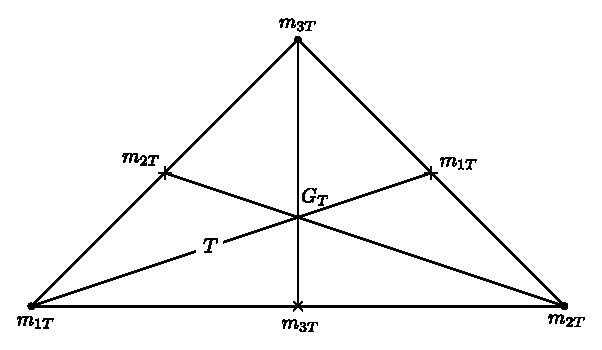
\includegraphics{vol65-figures/fig65-2.1.eps}}
\caption{}\label{c2:fig2.1}
\end{figure}
 
 The\pageoriginale  space $v = H^1 _0 (\Omega)$ is approximated by the
 family of 
 subspaces $(V^k_h)_h$ with $k=1$ or 2 where  
$$
V^k_h = \left\{ v_h \in C^0 (\overline{\Omega}) : v_h \big| _\Gamma = 0
~~\text{\em and } ~v_h \big|_T \in P_k ~\forall T \in \mathscr{C}_h
\right\}. k=1, 2. 
$$ 
 It is clear that $V^k_h$ are finite dimensional (cf. CIARLET [1]). It
 is then quite natural to approximate $K$ by  
$$
K^k_h = \left\{ v_h \in V^k_h : v_h (P) \geq \Psi (p)\ \forall P
\in \Sigma^k_h \right\}, k=1, 2. 
$$
 
\begin{proposition}\label{c2:prop2.1}%proposition 2.1
The $K^k_h$ for $k=1$, $2$ are closed, convex, non-empty subsets of $V^k_h$.
\end{proposition}

\begin{exercise}\label{c2:exer2.2}%exercise 2.2
Prove Proposition~\ref{c2:prop2.1}.
\end{exercise}

\subsubsection{The approximate problems }%subsubsection 2.5.2

For $k=1$, $2$ the approximate problems are defined by 
$$
(P^k_{1h})
\begin{cases}
a(u^k_h, v_h - u^k_h) \geq L (v_h - u^k_h)\, \forall v_h \in K^k_h,\\
u^k_h \in K^k_h.
\end{cases}
$$

From Theorem~\ref{c1:thm3.1} of Chapter~\ref{chap1} and 
Proposition~\ref{c2:prop2.1}, it follows that 

\begin{proposition}\label{c2:prop2.2}%proposition2.2.
$(P^k_{1h})$ has a unique solution for $k = 1$ and 2.
\end{proposition}

\begin{remark}\label{c2:rem2.3}%remark 2.3
If the bilinear form $a(\cdot ,\cdot)$ is symmetric, $(P^k_{1h})$ is
actually 
equivalent to (cf. Chap.~\ref{chap1}, Remark~\ref{c1:rem3.2}) the 
{\em quadratic programming} problem 
\begin{equation}
\min\limits_{v_h \in K^k_h} \left[ \frac{1}{2} a (v_h, v_h)-  L
  (v_h)\right]. \tag{2.24}\label{c2:eq2.24} 
\end{equation}

\subsection{Convergence results}\label{c2:ss2.6}%subsection 2.6

In other to simplify the convergence proof we shall assume in this
section that  
\begin{equation}
\Psi \in C^0 (\overline{\Omega}) \cap H^1 ~~\text{\em and }~~
\Psi \leq 0~~ \text{\em in a neighbourhood of
}~~\Gamma.\tag{2.25}\label{c2:eq2.25}  
\end{equation}
\end{remark}

Before\pageoriginale  proving the convergence results we shall give two important
numerical quadrature schemes which will be used to prove the
convergence theorem. 

\begin{exercise}\label{c2:exer2.3}%exercise 2.3.
With notations as in Fig.\ref{c2:fig2.1}, prove the following identities for any
triangle $T$ 
\begin{align}
&\int_T wdx = \frac{meas .(T)}{3} \sum\limits_{i=1}^{3} w(M_{iT})\,
  \forall w \in P_1.\tag{2.26}\label{c2:eq2.26}\\ 
&\int_T wdx = \frac{meas .(T)}{3} \sum\limits_{i=1}^{3} w(m_{iT})\,
  \forall w \in P_2.\tag{2.27}\label{c2:eq2.27} 
\end{align}
\end{exercise}
Formula~\eqref{c2:eq2.26} is called the \textit{Trapezoidal Rule} and
\eqref{c2:eq2.27} is known as \textit{Simpson's Integral formula}. These
formulae, not only have theoretical importance but also practical
utility.  

We have the following results about the convergence of $u^k_h$
(solutions of the problem ($P^k_h$)) as $h \to 0$. 

\begin{theorem}\label{c2:thm2.3}%theorem 2.3
Suppose that the angles of the triangles of $\mathscr{C}_h$ are uniformly
bounded below by $\theta _0 > 0$ as $h \to 0;$ then for $k=1$, 2 
\begin{equation}
\lim_{h \to 0} \parallel  u^k_h - u \parallel  _{H^1 _0(\Omega)} = 0 
\tag{2.28}\label{c2:eq2.28} 
\end{equation}
where $u^k_h$ and $u$ are respectively the solutions of $P^k_{1h}$ and
\eqref{c2:eq2.1}. 
\end{theorem}  

\begin{proof}
In this proof we shall use the following \textit{density} result to be\break
proved later: 
\begin{equation}
\overline{\mathscr{D} (\Omega) \cap K} =
K. \tag{2.29}\label{c2:eq2.29} 
\end{equation}
\end{proof}
  
To prove \eqref{c2:eq2.28} we shall use Theorem~\ref{c1:thm5.2}  of 
Chap.~\ref{chap1}.  To do this we
have to verify  that the following two properties hold (for $k=1$, 2): 
  
\begin{enumerate}[(i)]
\item If $(v_h)_h$ is such that $v_h \in K^k_h\, \forall  h$ and
  converges weakly to $v$ as $h \to 0$, then $v \in K$. 
\item There exists $\chi, \overline{\chi} = K$ and $r^k_h : \chi \to
  K^k_h$ such that $\lim\limits_{h \to 0} r^k_{h}v = v$
  =\textit{strongly } in $V\, \forall  v \in \chi$.  
\end{enumerate}
 
\medskip
\noindent\textbf{Verification of (i).}%varification of (i) 
 Using\pageoriginale  the notations of Fig.\ref{c2:fig2.1} and considering $\phi \in
 \mathscr{D}(\Omega)$ with $\phi \geq 0$, we define $\phi _h $ by
 $\phi_h = \sum\limits_{T \in \mathscr{C}_h } \phi (G_t ) \chi_T$
 where $\chi_T$ is the \textit{characteristic function} of $T$  and
 $G_T$ is the centroid of $T$. It is easy to see from the uniform
 continuity of $\phi$ that  
 \begin{equation}
\lim\limits_{h \to 0} = \phi~~ \text{\em strongly in }~~L^\infty
(\Omega).\tag{2.30}\label{c2:eq2.30}   
\end{equation}

Then we approximate $\Psi $ by $\Psi _h $ such that  
\begin{equation*}
\left\{\begin{aligned}
&\Psi_h \in C^0 (\overline{\Omega}), \Psi_h | _{T} \in P_k
\forall T \in \mathscr{C}_h,\\ 
&\Psi_h (P) = \Psi (P)\, \forall  P \in \Sigma^k_h. 
\end{aligned}\right.\tag{2.31}\label{c2:eq2.31}  
\end{equation*}

This function $\Psi_h$ satisfies
\begin{equation}
\lim\limits_{h \to 0} \Psi_h = \Psi ~~\text{\em strongly  in
}~~L^\infty (\Omega).\tag{2.32}\label{c2:eq2.32} 
\end{equation}
Let us consider a sequence $(v_h)_h$, $v_h \in K^k_h \, \forall  h$
such that  
$$
\lim\limits_{h \to 0} v_h = v~~ \text{\em weakly  in }~~V.
$$
Then $\lim\limits_{h \to o} v_h = v$ \textit{ strongly } in
$L^2(\Omega)$, (cf. NECAS [1]) which, using \eqref{c2:eq2.30} and
\eqref{c2:eq2.32}, implies that 
\begin{equation}
\lim\limits_{h \to 0} \int_\Omega (v_h - \Psi _h ) \Psi _h dx = \int
_\Omega (v - \Psi) \phi dx, \tag{2.33}\label{c2:eq2.33} 
\end{equation}
(actually since $\phi_h \to \phi$ \textit{strongly} in $L^\infty
(\Omega)$ the weak convergence of $v_h$ in $L^2(\Omega)$ is enough to
prove \eqref{c2:eq2.33}). 

We have 
\begin{equation}
\int_\Omega (v_h - \phi_h) \phi_h dx = \sum\limits_{T \in \subset
  _h} \phi (G_t) \int_T (v_h - \Psi_h) dx.\tag{2.34}\label{c2:eq2.34}  
\end{equation} 
From~\eqref{c2:eq2.26}. \eqref{c2:eq2.27} and the definition of
$\Psi_h$ we obtain for all $T \in  \mathscr{C}_h$. 
\begin{align}
&\int_T (v_h - \Psi_h ) dx = \frac{meas. (T)}{3} \sum\limits_{i=1}^{3}
[v_h (M_{iT}) - \Psi _h (M_{iT})] \text{ if } k=1,
\tag{2.35}\label{c2:eq2.35}\\  
&\int_T (v_h - \Psi_h ) dx = \frac{meas. (T)}{3} \sum\limits_{i=1}^{3}
[v_h (m_{iT}) - \Psi _h (m_{iT})] \text{ if } k=2,
\tag{2.36}\label{c2:eq2.36}  
\end{align}\pageoriginale  
 
Using the fact that $\phi_h \geq 0$, the definition of $K^k_h$ and the
relations \eqref{c2:eq2.35}, \eqref{c2:eq2.36} it follows from
\eqref{c2:eq2.34} that   
$$
\int_\Omega (v_h - \Psi_h) \phi_h ~dx \geq 0\, \forall  \phi \in
\mathscr{D} (\Omega), \phi\geq 0, 
$$
so that as $h \to 0$
$$
\int_\Omega (v - \Psi) \phi dx \geq 0\, \forall  \phi \in
\mathscr{D} (\Omega), \phi \geq 0 
$$
which in turn implies $v \geq \Psi $ a.e. in $\Omega$. Hence (i) is
verified. 

\medskip
\noindent \textbf{Verification of (ii).}%varification of (ii)
From \eqref{c2:eq2.29} it is natural to take $\chi = \mathscr{D} \cap
K$. We define $r^k_h : H^1 _0 (\Omega) \cap C^0 (\overline{\Omega})
\to V^k_h$ as the `` linear " interpolation operator when $k = 1$ and
`` quadratic" interpolation operator when $k=1$, i.e. 

 \begin{equation}
\begin{cases}
r^k_h v \in V^k_h\, \forall  v \in H^1 _0 (\Omega) \cap C^0
(\overline{\Omega}),\\ 
(r^k_h v )(p) = v (p)\, \forall  P \in \sum^{\circ k}_h ~\text{\em
  for }~~ k=1, 2. 
\end{cases}\tag{2.37}\label{c2:eq2.37} 
\end{equation}
 
On the one hand it is known (cf. for instance CIARLET [\ref{k31:e1}],
[\ref{k31:e2}] ,
STRANG-FIX [\ref{k85:e1}]) that under the assumptions made on $\mathscr{C}_h$ in
statement of Theorem \ref{c2:thm2.3} we have  
$$
\parallel  r^k_h v-v \parallel_v \leq C~ h^k \parallel  v \parallel_{H^{k+1}(\Omega)}\, \forall  v
\in \mathscr{D} (\Omega), k=1, 2. 
$$
with $C$ independent of $h$ and $v$ . This implies that 
$$
\lim_{h \to 0} \parallel  r^k_h v - v \parallel  _v = 0\, \forall  \in \chi, k=1,
2. 
$$
On the other hand it is obvious that 
$$
r^k_{h}v \in K^k_h\, \forall  v \in K \cap C^0
(\overline{\Omega}). 
$$
so that\pageoriginale  
$$
r^k_h v \in K^k_h\, \forall  v \in \chi, ~~\text{\em for }~~
k=1, 2. 
$$
 
In conclusion with the above $\chi$ and $r^k_h$, (ii) is
satisfied. Hence we have proved the Theorem~\ref{c2:thm2.3} modulo the
proof of the density result \eqref{c2:eq2.29}. 
 
\begin{lemma}\label{c2:lem2.4}%lemma 2.4
Under the assumptions \eqref{c2:eq2.25} we have
$\overline{\mathscr{D}(\Omega) \cap K} = K$. 
\end{lemma} 
 
\begin{proof}
Let us prove the Lemma in two steps.
\end{proof} 
 
\begin{step}\label{c2:st1}%step 1
Let us show that
\begin{equation}
\mathscr{K} = \{ v \in K \cap C^0 (\overline{\Omega}) : v
\text{compact support in } \Omega \}\tag{2.38}\label{c2:eq2.38} 
\end{equation} 
is \textit{dense} in $K$.
\end{step}
 
 Let $v \in K$, $K \subset H^1_0(\Omega) $ implies that exists a
 sequence $\{\phi_n\}_n$ in $\mathscr{D}(\Omega)$ such that   
$$
\lim_{n \to \infty} \phi_n = v~~ \text{\em strongly in }~~V.
$$
Define $v_n$ by 
\begin{equation}
v_n = \max (\psi, \phi_n) \tag{2.39}\label{c2:eq2.39}
\end{equation}  
so that 
$$
v_n = \frac{1}{2} [(\Psi + \phi_n) + |\Psi - \phi_n |].
$$
  
Since $v \in K$, from Corollary~\ref{c2:cor2.1} and 
relations \eqref{c2:eq2.39} i follows that 
\begin{equation}
\lim_{n \to \infty} v_n = \frac{1}{2} [(\Psi + v)+ |\Psi - v|] = \max
(\Psi, v) = v~~ \text{\em strongly in }~~V.\tag{2.40}\label{c2:eq2.40} 
\end{equation}  

From \eqref{c2:eq2.25} and \eqref{c2:eq2.39} it follows that 
\begin{align}
&\text{\em each } v_n  \text{ \em has a compact support in }\Omega,
  \tag{2.41}\label{c2:eq2.41}\\ 
&v_n \in K \cap C^0 (\overline{\Omega}). \tag{2.42}\label{c2:eq2.42}
\end{align}  
 From\pageoriginale  (\ref{c2:eq2.40}) - (\ref{c2:eq2.42}) we obtain
 (\ref{c2:eq2.38}) 
 
\begin{step}\label{c2:st2}%step 2
Let us show that 
\begin{equation}
\mathscr{D} (\Omega ) \cap \mathscr{K} is \text{ \em dense }
\mathscr{K}.\tag{2.43}\label{c2:eq2.43} 
\end{equation} 
\end{step} 
 
This proves from Step~\ref{c2:st1}, that $\mathscr{D}(\Omega) \cap K$ is dense in
$K$. Let $\rho_n$ be a sequence of mollifiers, i.e. 
\begin{equation}
\begin{cases}
\rho_n \in \mathscr{D} (\mathbb{R}^2), \rho_n \geq 0,\\
\int_{\mathbb{R}^2} \rho_n (y) dy = 1\\
\bigcap\limits^{\infty}_{n=1} \Supp \rho_n = \{0 \}, \{\Supp \rho_n \}
\text{is a decreasing sequence}. 
\end{cases}\tag{2.44}\label{c2:eq2.44}
\end{equation} 
Let $v \in \mathscr{K}$. Let $\tilde{v}$ extension of $v$ defined
by  
$$
\tilde{v}(x)=
\begin{cases} 
v (x) \text{ if } x \in \Omega,\\
0 \text{ if } x \notin \Omega,
\end{cases}
$$  
then $\tilde{v} \in H^1 (\mathbb{R}^2)$. Let $\tilde{v}_n =
\tilde{v} * \rho_n$ i.e. 
\begin{equation}
\tilde{v}_n (x) = \int_{\mathbb{R}^2} \rho_n (x - y) \tilde{v} (y) dy
\tag{2.45}\label{c2:eq2.45} 
\end{equation} 
then 
\begin{equation}
\begin{cases}
\tilde{v}_n \in \mathscr{D} (\mathbb{R}^2),\\
\Supp \tilde{v}_n \subset \Supp v + \Supp \rho_n'\\
\lim\limits_{n \to \infty} \tilde{v}_n = \tilde{v} \text{ strongly  in
}H^1 (\mathbb{R}^2). \tag{2.46}\label{c2:eq2.46}  
\end{cases}
\end{equation}
Hence from \eqref{c2:eq2.41} and \eqref{c2:eq2.46} we have   
\begin{equation}
\Supp (\tilde{v}_n) \subset \Omega \text{ for $n$ large
  enough}. \tag{2.47}\label{c2:eq2.47} 
\end{equation}

We also\pageoriginale  have (since $\Supp (\tilde{v})$is bounded) 
\begin{equation}
\lim \tilde{v}_n = \tilde{v} ~~\text{\em strongly in }~~L^\infty
(\mathbb{R}^2).\tag{2.48}\label{c2:eq2.48} 
\end{equation}
Define $v_n = \tilde{v}_n |_\Omega$, then 
\eqref{c2:eq2.46}--\eqref{c2:eq2.48} imply
\begin{equation}
\begin{cases}
v_n \in \mathscr{D}(\Omega)\\
\lim\limits_{n \to \infty } v_n  = v ~\text{\em strongly in}~ H^1_0 (\Omega)
\cap C^0 (\overline{\Omega}); \tag{2.49}\label{c2:eq2.49}   
\end{cases}
\end{equation}
$v \in \mathscr{K}$ and $\Psi \leq 0$ in a neighbourhood of
$\Gamma$ imply that there exists a $\delta > 0$ such that  
\begin{equation}
v = 0, \Psi \leq 0 ~\text{\em on }~ \Omega_\delta
\tag{2.50}\label{c2:eq2.50} 
\end{equation}
where $\Omega_\delta = \{x \in \Omega : d(x, \Gamma) < \delta \}$.

From \eqref{c2:eq2.48} and \eqref{c2:eq2.50} it follows that $\forall
\in > 0$, there exists an $n_0 = n_0 (\in)$ such that
$\forall n \geq n_0 (\in)$ 
\begin{equation}
\begin{cases}
v (x) - \in \leq v_n (x) \leq (x) + \in\, \forall  x \in
\Omega-\Omega_{\delta / 2}\\ 
v_n (x) = v(x) = 0 \text{ for } x \in \Omega_{\delta/2}
\end{cases}\tag{2.51}\label{c2:eq2.51} 
\end{equation}
Since $\overline{\Omega} - \Omega_{\delta / 2}$ is a compact subset of
$\overline{\Omega}$ there exists a functions $\theta$ (cf. for
instance $H$. CARTAN [\ref{k25:e1}]) such that  
\begin{equation}
\begin{cases}
\theta \in \mathscr{D} (\Omega),  \theta \geq 0~\text{\em in }
\Omega\\ 
\theta (x) = 1\, \forall  x \in \overline{\Omega} - \Omega_{\delta
  /2 }\tag{2.52}\label{c2:eq2.52}  
\end{cases}
\end{equation}
Finally define $w^\epsilon  _n =  v_n + \in \theta$.

Then from \eqref{c2:eq2.49}, \eqref{c2:eq2.51} and \eqref{c2:eq2.52}
we have  
$$
w^\epsilon  _n \in \mathscr{D} (\Omega)
$$ 
$$
\lim_{\substack{\in \to 0 \\ n \to \infty \\ n \geq n_0
    (\in)}} 
w^\epsilon  _n = v~~ \text{\em strongly in }~~ H^1_0(\Omega), 
$$
with\pageoriginale  $w^\epsilon _n (x) \geq v (x) \geq \Psi (x)\,
\forall  x \in \Omega$, so that Step~\ref{c2:st2}, is proved. 

\begin{remark}\label{c2:rem2.4}%remark 2.4
Analysing the verification (i) in the  proof of {\small Theorem~\ref{c2:thm2.3}}, we
observe that if for $k=2$ we use, instead of $K^2_h$, the following
convex set  
$$
\{v_h \in V^2_h : v_h (p) \geq \Psi (p)\, \forall  P \in
\sum^{0}{}'_h \} 
$$ 
then the convergence of $u^2_h$ to $u$ still holds provided $\mathscr{C}_h$
obeys the same assumptions as in the statement of Theorem~\ref{c2:thm2.3}. 
\end{remark}

\begin{exercise}\label{c2:exer2.4}%exercise 2.4.
Extend the previous analysis if $\Omega $ is not a polygonal domain.
\end{exercise}

\begin{exercise}\label{c2:exer2.5}%exercise 2.5
Let $\Omega$ be a bounded domain of $\mathbb{R}^2$ and $\Gamma_0$ a
``nice'' subset of $\Gamma$, see Fig.~2.2. Define $V$ by $V = \{v
\in H^1 (\Omega) : v|{\Gamma_0 } = 0 \}$. Taking the bilinear
form $a(\cdot , \cdot)$ like in  \eqref{c2:eq2.1}, and $L \in V^*$, study
the following EVI 
$$
\begin{cases}
a (u, v - u)\geq L(v - u)\, \forall  v \in K,\\
u \in K,
\end{cases}
$$
\end{exercise}
where $K = \{v \in V : v \geq  \Psi$ a.e. in $\Omega \}$ and
$\Psi \in C^0 (\overline{\Omega}) \cap H^1 (\Omega)$, $\Psi \leq
0$ in a neighbourhood of $\Gamma_0$. Also study the finite element
approximation of the above EVI. 

\textbf{Hint}. Use the fact that if $\Gamma$ and $\Gamma_0$ are smooth
enough then $\mathscr{V} = V$ where (see Fog.~2.2) $\mathscr{V}  = \{v
\in C^\infty (\overline{\Omega}) : v = 0$ in a neighbourhood of
$\Gamma_0 \}$.  

\begin{figure}[H]
\centering{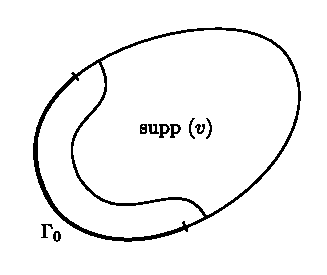
\includegraphics{vol65-figures/fig65-2.2.eps}}
\caption{}
\end{figure}

\subsection{Comments on the error estimates}\label{c2:ss2.7}

We do not\pageoriginale  emphasize too much on this subject since it
has been done in 
detail in CIARLET [\ref{k31:e1}], Chap.9, at least for piecewise linear
approximations. 

\subsubsection{Piecewise linear approximation}\label{c2:sss2.7.1}
%subsubsection 2.7.1 

Using piecewise linear finite elements and assuming that $f $, $\Psi$,
$u \in H^2 (\Omega)$, $0(h)$ estimates for $\parallel  u-u_h
\parallel_{H^1(\Omega)}$ have been obtained by FALK[\ref{k44:e1}],
[\ref{k44:e2}], [\ref{k44:e3}], STRANG [\ref{k84:e1}],
STRANG-MOSCO [\ref{k86:e1}]. We also refer to CLARLET [\ref{k31:e1},
  Chap. 9], in which the Falk analysis is given.  

\subsubsection{Piecewise quadratic approximation}\label{c2:sss2.7.2}%subsubsection 2.7.2 
 Assuming more regularity for $f$, $\Psi$, $u$ that in the previous
 case, assuming also some smoothness hypotheses for the free boundary,
 an $0(h^{3/2-\epsilon})$ estimate for $\parallel  u_h - u\parallel_{H61(\Omega)}$ has
 been obtained by BREZZI-HAGER-RAVIART [\ref{k18:e1}], BREZZI-SACCHI
 [\ref{k20:e1}] for an
 approximation by piecewise quadratic finite elements, similar to the
 described in Section~\ref{c2:ss2.6}. 

\subsection{Iterative solution of the approximation
  problem}\label{c2:ss2.8}%subsection 2.8. 

Once the continuous problem has been approximated and the convergence
proved, it remains to compute effectively  the approximate
solution. In the case of the discrete obstacle problem this can be
done easily by using an \textit{over- relaxation method with
  projection} as described in CEA[2]. 

Let us justify the use of this method. It follows from
Remark~\ref{c2:rem2.3} that the discrete problem is of the following type 
\begin{equation}
\min_{v \in C} \left[\frac{1}{2} (Av, v) - (b, v) \right
]\tag{2.53}\label{c2:eq2.53} 
\end{equation}
where $(\cdot ,\cdot)$ denotes the usual inner product in
$\mathbb{R}^N$ and $v = \{v_1, \ldots, v_n \}$ and  
\begin{equation}
A = (a_{ij}), 1 \leq i \leq N, 1 \leq j \leq
N\tag{2.54}\label{c2:eq2.54}  
\end{equation}
is a symmetric, positive definite $N \times N$ and $C$ is the set
given by  
\begin{equation}
C = \{v \in \mathbb{R}^N : v_i \geq \Psi_i, 1 \leq i \leq N
\}. \tag{2.55}\label{c2:eq2.55} 
\end{equation}

Since\pageoriginale  $C$ is the product of closed intervals of $\mathbb{R}$, the
over-relaxation method with projection on $C$ can be used. Let us
describe it in detail: 
\begin{align*}
u^0 & \in C, u^0  ~\text{\em arbitrarily chosen in } ~~C \\
(u^0 &  = \{\Psi_1, \ldots, \Psi_n \} ~~\text{\em may be a good
  guess}). \tag{2.56}\label{c2:eq2.56} 
\end{align*}
\textit{Then} $u^n$ \textit{being known, we compute} $u^{n+1}$,
\textit{component by component using for } $i =1$, $2, \ldots N$ 
\begin{align}
u^{-n +1}_{i} = \frac{1}{a_{ii}} \left( b_i - \sum\limits^{i-1}_{j=1}
a_{ij} u^{n+1}_{j} - \sum\limits^{N}_{j=i+1} a_{ij} u^n_j
\right).\tag{2.57}\label{c2:eq2.57}\\ 
u^{n+1}_{i} = P_i (u^n_i + w (u^{-n+1}_{i} -u^n_i))\tag{2.58}\label{c2:eq2.58}  
\end{align}
where 
\begin{equation}
P_i (x) = \max (x, \Psi_i)\, \forall  x \in
\mathbb{R}.\tag{2.59}\label{c2:eq2.59}  
\end{equation}

It follows from CEA [\ref{k27:e2}] (see also CEA-GLOWINSKI
[\ref{k53:e1}], G.L.T. [1] )that 

\begin{proposition}\label{c2:prop2.3}%proposition 2.3
Let $(u^n)$ be defined by \eqref{c2:eq2.56}--\eqref{c2:eq2.59}. Then
for every 
$u^0 \in C$ and $\forall 0 < w < 2$, we have $\lim\limits_{n \to
  \infty} u^n = u$ where $u$ is the unique solution of \eqref{c2:eq2.53}. 
\end{proposition}

\begin{remark}\label{c2:rem2.5}%remark 2.5
In the case of the discrete obstacle problem the components of $u$
will be the values taken by  the approximation solution at the nodes
of $\sum\limits^{0}_{h}$ if $k =1$ and $\sum\limits^{0}_{h} \cup
\sideset{}{'}\sum\limits^0_h$  if $k
-2$. Similarly $\Psi_i$ will be the values taken by $\Psi$ at the
nodes stated above, assuming these nodes have been ordered from 1 to
$N$. 
\end{remark}

\begin{remark}\label{c2:rem2.6}%remark 2.6
The optimal choice for $\omega$ is a critical but nontrivial
point. However it has been observed from numerical experiments that
the so-called {\em Young method} for obtaining the optimal value of
$\omega$ during the iterative process itself, leads to a value of
$\omega$ with good convergence properties. The convergence of this
method has been proved for linear equations and requires special
properties for the matrix of the system (see YOUNG  [\ref{k92:e1}], VARGA
[\ref{k90:e1}]). However, empirical justification of its  success for
the obstacle problem can be made, but will not be given here. 
\end{remark}

\begin{remark}\label{c2:rem2.7}%Remk 2.7 
From numerical experiments it is found that the optimal value of
$\omega$ is always strictly greater than one. 
\end{remark}

\section[A Second Example of EVI of The...]{A Second Example of EVI of
  The First Kind: The   Elasto-Plastic Torsion
  Problem}\label{c2:s3}%section  3.  

\subsection{Formulation. Preliminary results}\label{c2:ss3.1}%subsection 3.1

Let\pageoriginale  $\Omega$ be a bounded domain of $\mathbb{R}^2$ with
a smooth 
boundary $\Gamma$. With the same definition for $V$, $a(\cdot ,
\cdot)$, $L(.)$ 
as in Sec.~\ref{c2:ss2.1} of this Chapter, we consider the following
EVI of the 
first kind 
\begin{equation}
\begin{cases}
a(u, v-u) \geq L(v - u)\, \forall  v \in K,\\
u \in K,\tag{3.1}\label{c2:eq3.1}
\end{cases}
\end{equation}
where 
\begin{equation}
K = \{v \in H^1_0 (\Omega) : | \nabla _v | \leq 1
a.e. \text{ in } \Omega \}. \tag{3.2}\label{c2:eq3.2} 
\end{equation}

\begin{theorem}\label{c2:thm3.1}%theorem 3.1
Problem \eqref{c2:eq3.1} has a unique solution.
\end{theorem}

\begin{proof}
In order to apply Theorem~\ref{c1:thm3.1} of Chapter I, we only have
to verify that $K$ is a {\em non- empty, closed, convex}, subset of
$V$.  
\end{proof}

$K$ is non-empty because $0 \in K$, and the convexity of $K$ is
obvious. To prove that $K$ is closed, consider a sequence $\{v_n \}$
in $K$ such that $v_n \to v$ strongly in $V$. Then there exists a
subsequence $\{v_{n_i}\}$ such that  
$$
\lim_{i \to \infty} \nabla v_{n_i} = \nabla v~\text{a.e.} 
$$

Since $| \nabla v_n | \leq 1$ a.e. we get $| \nabla v |
\leq 1$ a.e. therefore $v \in K$. Hence $K$ is closed. 

The following Proposition gives a very useful property of $K$. 

\begin{proposition}\label{c2:prop3.1} % prop 3.1
$K$  is compact in $C^0 (\bar{\Omega})$ and 
\begin{equation}
| v (x) | \leq \dot{d} (x, \Gamma)\, \forall  x \in \Omega \text
{ and }\, \forall  v \in K,\tag{3.3}\label{c2:eq3.3} 
\end{equation}
where $d (x, \Gamma)$ is the distance from $x$ to $\Gamma$.
\end{proposition}

\begin{exercise}\label{c2:exer3.1}%exercise 3.1
Prove\pageoriginale  Proposition~\ref{c2:prop3.1}
\end{exercise}

\begin{remark}\label{c2:rem3.1}% remark 3.1
Let us define $u_\infty$ and $u_{-\infty}$ by 
\begin{gather*}
u_\infty (x) = d(x, \Gamma)\\
u_{-\infty} (x) = -d(x, \Gamma).
\end{gather*}
\end{remark}

Then $u_{\infty}$ and $u_{-\infty}$ to $K$. We observe that $u_\infty$
is the \textit{maximal} element of $K$ and $u_{-\infty}$ is the
\textit{minimal} element of $K$. 

\begin{remark}\label{c2:rem3.2}%remark 3.2
Since $a(\cdot , \cdot)$ is {\em symmetric} the solution $u$ of \eqref{c2:eq3.1} is
characterised (see Section~\ref{c2:ss3.2} of Chap.~\ref{chap1}) as the unique solution of
the minimization problem 
\begin{equation}
\begin{cases}
J(u) \leq J(v) ~\forall v \in K,\\
u \in K, 
\end{cases}\tag{3.4}\label{c2:eq3.4}
\end{equation}
with $J(v) = \dfrac{1}{2} a(v, v) - L (v)$.
\end{remark}

\subsection{Physical motivation}\label{c2:ss3.2}%subsection 3.2

 Let us consider an infinitely long cylindrical bar of cross-section
 $\Omega$ where $\Omega$ is \textit{simply connected}. Assume that
 this is made up of an \textit{isotro\-pic, elastic, perfectly plastic}
 material whose plasticity yield is given by the Von Misses
 Criterion. (For a general discussion of plasticity problems, see
 KOITER [\ref{k62:e1}], DUVAUT-LIONS [\ref{k42:e1},
   Chap. 5]). Starting from a \textit{zero 
   stress initial state}, an increasing \textit{torsion} moment is
 applied to the bar. The torsion is characterised by $C$ which is
 defined as the \textit{torsion angle per unit length}. Then for all
 $C$, it follows from the \textit{Harr- Karman Principle} that the
 determination of the \textit{stress field} is equivalent (in a
 convenient system of physical units) to the solution of the following
 variational problem:  

\begin{equation}
\min_{v \in K} \frac{1}{2} \int_\Omega |\nabla _v |^2
dx - C \int_\Omega v dx.\tag{3.5}\label{c2:eq3.5} 
\end{equation}  
  
This is a particular case of \eqref{c2:eq3.1} 
or \eqref{c2:eq3.4} with 
\begin{equation}
L (v) = C \int_\Omega v dx.\tag{3.6}
\end{equation} 
  
 The\pageoriginale  \textit{stress vector} $\sigma$ in a cross - section  is related
 to $u$ by $\sigma = \nabla u$, so that $u$ is a
 \textit{Stress potential} and we obtain $\sigma$ once the solution of
 \eqref{c2:eq3.5} is known.  
  
\begin{proposition}\label{c2:prop3.2}%proposition 3.2.
Let us denote by $u_C$ the solution of \eqref{c2:eq3.5} and let, as before
$u_\infty =  d(x, \Gamma)$ then $\lim\limits_{C \to \infty} u_C =
u_\infty$ strongly in $H^1_0 (\Omega) \cap C^0 (\overline{\Omega})$. 
\end{proposition} 
  
\begin{proof}
Since $u_C$  is the solution of (\ref{c2:eq3.5}), it is characterised by 
\begin{equation}
\begin{cases}
\int_\Omega \nabla u_C . \nabla (v - u_C) dx \geq
C \int_\Omega (v - u_C) dx\, \forall  v \in K,\\ 
u_C \in K.\tag{3.7}\label{c2:eq3.7}
\end{cases}
\end{equation}
\end{proof}
Since $u_\infty \in K$, from \eqref{c2:eq3.7} we have 
\begin{equation}
\int_\Omega \nabla u_C. \nabla (u_\infty - u_C) dx
\geq C \int_\Omega (u_\infty - u_C )dx, \tag{3.8}\label{c2:eq3.8} 
\end{equation}
i.e.
\begin{equation}
\begin{cases}
C \int_\Omega (u_\infty - u_C) dx + \int_\Omega | \nabla u_C
| ^2 dx \leq \int_\Omega \nabla u_\infty. \bigtriangledown
u_C dx \\ 
\leq \int_\Omega | \nabla u_\infty | . \nabla u_C
| dx \leq (\text{ meas }. \Omega ). 
\end{cases}\tag{3.9}\label{c2:eq3.9} 
\end{equation} 
From \eqref{c2:eq3.3} we have $u_\infty - u_C \geq 0$ 
so that \eqref{c2:eq3.9} implies
$$
\parallel  u_\infty - u_C \parallel  _{L^1 (\Omega)} \leq C^{-1} 
(\text{ meas}. \Omega). 
$$  
Which in turn implies 
\begin{equation}
\lim_{C \to \infty } \parallel  u_\infty - u_C \parallel  _{L^1 (\Omega)} =
0. \tag{3.10}\label{c2:eq3.10} 
\end{equation}

Form the definition of $K$ and from the Proposition~\ref{c2:prop3.1} we get that
$K$ is bounded and weakly closed in $V$ and hence weakly compact  in
$V$. Further $K$ is compact in $C^0 (\overline{\Omega})$.  

Relation~\eqref{c2:eq3.10} implies 
\begin{equation}
\begin{cases}
\lim\limits_{C\to \infty} u_C  & = u_\infty ~~ \text{\em strongly in }
C^0 (\overline{\Omega}),\\ 
\lim\limits_{C \to \infty} u_C & = u_\infty~~  \text{\em weakly in }V.
\end{cases}\tag{3.11}\label{c2:eq3.11} 
\end{equation}\pageoriginale 
It follows from \eqref{c2:eq3.8} that 
\begin{equation}
 \begin{cases}
\int_\Omega \nabla u_\infty. \nabla (u_\infty - u_C ) \geq \int_\Omega
| \nabla (u_\infty - u_C) | ^2 dx + C \int_\Omega (u_\infty - u_C )dx
\\ 
= \parallel  u_C - u_\infty \parallel  ^2 _V + C \parallel  u_\infty - u_C \parallel  _{L^1(\Omega)}.
\end{cases}\tag{3.12}\label{c2:eq3.12}
\end{equation}  
 It follows easily from \eqref{c2:eq3.11} and \eqref{c2:eq3.12} that 
\begin{align*}
&\lim_{C \to \infty} C \parallel  u_\infty - u_C \parallel  _{L^1 (\Omega)} = 0,\\
&\lim_{C \to \infty} \parallel  u_\infty - u_C \parallel  _V = 0. 
\end{align*} 
 
\begin{remark}\label{c2:rem3.3}%remark 3.3
In the case of multiply connected cross section, the variational
formulation of the torsion problem has to redefined (see LANCHON
[\ref{k52:e1}], 
GLOWINSKI - LANCHON [\ref{k63:e1}], GLOWINSKI [\ref{k51:e1}, Chap 4]). 
\end{remark}
  

\subsection{Regularity properties and exact solutions}\label{c2:ss3.3}%subsection 3.3
  
\subsubsection{Regularity results}\label{c2:sss3.3.1}%subsubsection 3.3.1 
  
\begin{theorem}\label{c2:thm3.2}%theorem 3.2
(BREZIS-STAMPACCHIA [2]). Let $u$ be a solution of \eqref{c2:eq3.1} or 
\eqref{c2:eq3.4} and $L (v) = \int_\Omega fv\,dx$. 
\end{theorem}
  
\begin{enumerate}[(1)]
\item \textit{Let $\Omega$ be a bounded convex domain of
  $\mathbb{R}^2$ with $\Gamma$ Lipschitz continuous and $f \in L^p
  (\Omega)$ with $1< p < \infty$. Then we have}  
 
\begin{equation}
u \in W^{2, p} (\Omega). \tag{3.13}\label{c2eq3.13}
\end{equation}  
\item  \textit{If $\Omega$ is a bounded domain of $\mathbb{R}^2$ with
a smooth boundary $\Gamma ;$ if $f \in  L^p(\Omega)$ with $1 <
p < \infty $ then $u \in W^{2, p}(\Omega)$ .} 
\end{enumerate}  

\begin{remark}\label{c2:rem3.4}%remark 3.4
It will\pageoriginale  be seen in the next section that, in general, there is a limit
for the {\em regularity}of the {\em solution} of \eqref{c2:eq3.1} even if
$\Gamma$ and $f$ are very smooth. 
\end{remark}

\begin{remark}\label{c2:rem3.5}%remark3.5
It has been proved by H. BREZIS that, under quite restrictive
smoothness assumptions on $\Gamma$ and $f$ we may have  
$$
u \in W^{2, \infty}(\Omega).
$$
\end{remark}

\subsubsection{Exact solutions}\label{c2:sss3.3.2}%subsubsection 3.3.2

 In this section we are going to give some examples of problems \eqref{c2:eq3.1}
 for which exact solutions are known. 

\begin{example}\label{c2:ex1}%example 1
We take $\Omega = \{x : 0 < x < 1 \}$ and $L (v) = C \int^1_0 v ~ dx $
with $c > 0$. 

Then the explicit form \eqref{c2:eq3.1} is 
\begin{equation}
\begin{cases}
\int^1_0 u' (v' - u') dx \geq c \int^1_0 (v - u) dx\, \forall  v \in K,\\
u \in K,\tag{3.14}\label{c2:eq3.14}
\end{cases}
\end{equation}
where $K = \{v \in H^1_0 (\Omega) : | v'| \leq 1$ a.e. on $\Omega
\}$ and $v' = \dfrac{dv}{dx}$.  
\end{example}

The exact solutions of (\ref{c2:eq3.14}) is given by
\begin{equation}
 u (x) = \frac{c}{2} x(1 - x)\, \forall  x, \text{ if } c \leq
 2. \tag{3.15}\label{c2:eq3.15} 
 \end{equation}
 If $c > 2$
 \begin{equation}
u(x)=
\begin{cases}
x \text{ if } 0 \leq x \leq \frac{1}{2} - \frac{1} {c}\\
\frac{c}{2} [x(1 - x) - (\frac{1}{2} - \frac{1}{c})] \text{ if }
\frac{1}{2} - \frac{1}{2} \leq x \leq \frac{1}{2} + \frac{1}{2},\\ 
1 - x \text{ if } \frac{1} {2} + \frac{1}{c} \leq x \leq 1.
\tag{3.16}\label{c2:eq3.16} 
\end{cases}
 \end{equation} 
 
\begin{example}%example 2
In this example we consider a two dimensional problem. We take 
\begin{gather*}
\Omega = \{x : x^2_1 + x^2_2 < R^2 \},\\
L(v) = c \int_\Omega v dx \text{ with } c > 0.
\end{gather*}
\end{example} 
 
 Then\pageoriginale  setting $r = (x^2_1 + x^2_2)^{1/2}$ the solution $u$ of \eqref{c2:eq3.1} is  given by  
 \begin{equation}
 u (x) = \frac{c}{4} (R^2 - r^2) \text{ if } c \leq
 \frac{2}{R},\tag{3.17}\label{c2:eq3.17} 
 \end{equation}
 if $c > \dfrac{2}{R}$ then 
 \begin{equation}
u(x)=
\begin{cases}
R - r \text{ if }\frac{2}{c} \leq r \leq R,\\
\frac{c}{4} [(R^2 - r^2) - (R - \frac{2}{c})^2 ] \text{ if } 0 \leq r
\leq \frac{c}{2}.\tag{3.18}\label{c2:eq3.18} 
\end{cases}
 \end{equation} 
 These examples illustrate Remark \ref{c2:rem3.4}. We see that for $c$ large
 enough we have  
 \begin{equation}
u \in W^{2, \infty} (\Omega) \cap H^1_0 (\Omega), u \notin H^3
(\Omega). \tag{3.19}\label{c2:eq3.19} 
 \end{equation} 
 In fact we have 
 $$
 u \in H^s (\Omega)\, \forall  s < \frac{5}{2}.
 $$
 \begin{exercise}%exercise 3.2
Verify that $u$ given in the above two examples are exact solutions of
the corresponding problems. 
 \end{exercise} 
 
 \subsection{An equivalent variational 
formulation}\label{c2:ss3.4}%subsection 3.4 
 
 In H. BREZIS-M, SIBONY [1] it is proved that if $\Omega$ is a bounded 
 domain of $\mathbb{R}^2$ with a smooth boundary $\Gamma$ and if    
 $$
 L(v) = c \int_\Omega v (x) ~ dx (c > 0 ~\text{\em for instance}),
 $$
\begin{equation}
\begin{cases}
a (u, v - u) \geq c \int (v - u) dx ~\forall v \in \hat{K},\\
u \in \hat{K} = \{v \in H^1_0 (\Omega), | v (x) | \leq d (x,
\Gamma)  a.e. \}.\tag{3.20}\label{c2:eq3.20} 
\end{cases}
\end{equation} 
 
 The above problem \eqref{c2:eq3.20} is very similar to the obstacle problem
 considered in Sec.~\ref{c2:s2} of this Chapter. Since $a(\cdot , \cdot)$ is symmetric,
 \eqref{c2:eq3.20} is also equivalent to  
 \begin{equation}
\begin{cases}
J(u) \leq J(v) ~~\, \forall  v \in \hat{K},\\
u \in \hat{K}, \tag{3.21}\label{c2:eq3.21}
\end{cases}
\end{equation}\pageoriginale  
 with
 $$
 J (v) = \dfrac{1}{2} a (v, v) - c \int_\Omega v (x) dx.
 $$
 The numerical solutions of \eqref{c2:eq3.20} and \eqref{c2:eq3.21} is
 considered in G.L.T [1, Chap.~3] (see also CEA[2, Chap. 4]). 
 
\begin{exercise}%exercise 3.3
Study the numerical analysis of \eqref{c2:eq3.21}.
\end{exercise} 
 
\begin{exercise}%exercise 3.4
Assume $c > 0$ in \eqref{c2:eq3.20}. Then prove that the solution $u$ of \eqref{c2:eq3.20}
is also the solution of the EVI obtained by replacing $K$ by $\{v
\in H^1_0 (\Omega)  : v (x) \leq d (x, \Gamma) a.e. \}$ in
\eqref{c2:eq3.20}. 
 \end{exercise} 
 
\subsection{Finite Element Approximations of (\ref{c2:eq3.1}).}%subsection 3.5
 
 We consider in this section an approximation of (\ref{c2:eq3.1}) be 
\textit{first order finite elements}. From  the view point of applications
 in mechanics (in which $f = c$) it seems that, given the equivalence
 of \eqref{c2:eq3.1} and \eqref{c2:eq3.20}, it is sufficient to
 approximate 
 \eqref{c2:eq3.20} (using
 essentially the same method as in Sec.~\ref{c2:s2}). However, in  view of other
 possible applications, it seems to us that it would be interesting to
 consider the numerical solution  of \eqref{c2:eq3.1} working directly with $K$
 instead of $\hat{K}$. For the numerical analysis of \eqref{c2:eq3.20} by Finite
 Differences sec G.L.T. [1. Chap. 3] and CEA-GLOWINSKI-NEDELEC [\ref{k29:e1}]. 
 
 \subsubsection{Approximation of V and K.}\label{c2:sss3.5.1}%sub sec 3.5.1
 
 We use the notation of Sec.~\ref{c2:ss2.5} of this Chap. We assume that $\Omega$
 is a polygonal domain of $\mathbb{R}^2$ (see Remark  \ref{c2:rem3.8} below for
 the non polygonal case) and we consider a triangulation $\tau_h$ of
 $\Omega$ satisfying \eqref{c2:eq2.21}--\eqref{c2:eq2.23}. Then $V $
 and $K$ are respectively approximated by  
 \begin{align*}
v_h  &= \{v_h \in C^0 (\overline{\Omega}) : v_h = 0 \text{ on }
\Gamma, v_h | _T \in P_1\, \forall  T \in \tau_h \},\\ 
K_h & = K \cap V_h
\end{align*}
Then one can easily prove

\begin{proposition}\label{c2:prop3.3}%proposition 3.3
$K_h$ is\pageoriginale  a closed, convex, non-empty subset of $V_h$.
\end{proposition}

\begin{remark}\label{c2:rem3.6}%remark 3.6
If $v_h \in V_h$ then $\nabla v_h$ is a constant vector
on every $T \in \tau_h$. 
\end{remark}

\subsubsection{The approximate problem}\label{c2:sss3.5.2}%sub sec
                                %3.5.2 

The approximate problem is defined by : 
\begin{equation}
\begin{cases}
\text{ Find } u_h \in K_h \text{ such that }\\
a (u_h, v_h - u_h) \geq L (v_h - u_h)\, \forall  v_h \in
K.\tag{3.22}\label{c2:eq3.22}  
\end{cases}
\end{equation} 
One can easily prove

\begin{proposition}\label{c2:prop3.4}%proposition 3.4
The approximate problem \eqref{c2:eq3.22} has a unique solution.
\end{proposition}  
  
  One may find in Sec~\ref{c2:s7}. of this chapter practical  formulae related
  to finite element approximation. Using these formulae, \eqref{c2:eq3.22} and
  the equivalent problem \eqref{c2:eq3.23} can be expressed in a form more
  suitable for computation. 
  
\begin{remark}\label{c2:rem3.7}%remark 3.7
Since  $a(\cdot , \cdot)$ is symmetric, \eqref{c2:eq3.22} is equivalent to the
non-linear programming problem  
\begin{equation}
\min\limits_{v_h \in K_h} \left [ \frac{1}{2} a (v_h, v_h) - L
  (v_h) \right].\tag{3.23}\label{c2:eq3.23} 
\end{equation}
\end{remark} 
  
  The natural variables in \eqref{c2:eq3.23} are the values taken by $v_h$ over
  the set $\sum\limits^{0}_{h}$ of the interior nodes of
  $\tau_h$. Then the number of variables in \eqref{c2:eq3.23} is Card
  $(\sum\limits^{0}_{h})$. The number of constraints is the number of
  triangles i.e. Card $(\tau_h)$ and each constraint is quadratic
  w.r.t. the variables since  
  \begin{equation}
| \nabla v_h | \leq 1 \text{ iff } | \nabla v_h |
^2 \leq 1 \text{ over T}.\tag{3.24}\label{c2:eq3.24} 
 \end{equation} 
 
\begin{remark}\label{c2:rem3.8}%remark 3.8
If $\Omega$ is not polygonal, it is always possible to approximate
$\Omega $ by a polygonal domain $\Omega_h$ in such a way that all
vertices of $\Gamma_h = \partial \Omega_h$ belong to $\Gamma$. Then
instead of defining \eqref{c2:eq3.22} over $\Omega$ we define it over
$\Omega_h$. 
\end{remark}  
  
\subsubsection{Remarks on the use of 
higher order finite elements}\label{c2:sss3.5.3}%sub sec 3.5.3.
  
  In these notes only an approximation of \eqref{c2:eq3.1} by first order finite
  elements has been considered. That fact is justified by the
  existence of a \textit{regularity limitation} for the solution of
  \eqref{c2:eq3.2}, which implies that even very smooth data one may have $u
  \notin V\cap H^3 (\Omega)$ (see examples of Sec.~\ref{c2:sss3.3.2}. 
  
  We refer\pageoriginale  to G.L.T. [1, Chap. 3] and GLOWINSKI [1, Chap
    . 4. Sec. 3.5.3] for further discussions on the use of finite
  elements of order $\geq 2$. 
  
  \subsection{Convergence results . General case}\label{c2:ss3.6}%section 3.6
  
  In this sections we take $L (v) = <f, v>$, for $f \in H^{-1}(\Omega) = V$.
  
  \subsubsection{A density Lemma}\label{c2:sss3.6.1} %subsub sec 3.6.1
  
  In order to apply the general results of Chap.~\ref{chap1}, the following
  density lemma will be very useful 
  
\begin{lemma}\label{c2:lem3.1}%lemma 3.1
We have 
\begin{equation}
\overline{\mathscr{D} (\Omega) \cap K} = K.\tag{3.25}\label{c2:eq3.25}
\end{equation}
\end{lemma}  
  
\begin{proof}
We use the notation of Lemma~\ref{c2:lem2.4}. Let $v \in K$ and $
\in > 0$; define $v_\epsilon $ by  
\begin{equation}
v_\epsilon = (v - \in)^+ - (v + \in)^-.\tag{3.26}\label{c2:eq3.26} 
\end{equation}
\end{proof}  
 Then we have $v_\epsilon \in H^1(\Omega)$ with $|\bigtriangledown
 v_\epsilon | \leq 1$ a.e. in $\Omega$. From the inclusion $K \subset
 \hat{K} = \{v \in V : | v (x) | \leq d (x, \Gamma)$ a.e. in
 $\Omega \}$ it follows that  
\begin{equation}
\begin{cases}
v_\epsilon (x) = 0 \text{ if } d (x, \Gamma) \leq \in,\\
|v_\epsilon (x)| \leq d (x, \Gamma) - \in ~~\text{\em elsewhere
}\tag{3.27}\label{c2:eq3.27}  
\end{cases}
\end{equation}
so that from \eqref{c2:eq3.27} it follows that 
\begin{equation}
v_\epsilon \in K \text{\em and has a compact support in }
\Omega. \tag{3.28}\label{c2:eq3.28} 
\end{equation}
From Corollary~\ref{c2:cor2.1} we have 
\begin{equation}
\lim_{\in \to 0} v_\epsilon = v~~ \text{\em strongly in
}~~V.\tag{3.29}\label{c2:eq3.29}   
\end{equation}
From \eqref{c2:eq3.28} and \eqref{c2:eq3.29} it follows that if
$\mathscr{K} = \{v \in K : v$ has a compact support in
$\Omega\}$, then $\mathscr{K} = K$.  

Thus to prove the lemma it suffices to prove that any $v \in
\mathscr{K}$ can be approximated by a sequence $(v_n)_n$ of functions
in $\mathscr{D}(\Omega) \cap K$. Let $\rho_n$ be a mollifying sequence
as defined\pageoriginale  in Lemma~\ref{c2:lem2.4} of this chapter. Let $v \in
\mathscr{K}$. Denote by $\tilde{v}$ extension of $v$ to $\mathbb{R}^2$
putting outside $\Omega$. Then $\tilde{v} \in
H^1(\mathbb{R}^2)$. 

Let $ \tilde{v}_n = \tilde{v}* \rho_n$  so that 
  \begin{gather}
\tilde{v}_n (x) = \int\limits_{\mathbb{R}^2} \rho_n (x - y) \tilde{v}
(y)dy, \tag{3.30}\label{c2:eq3.30}\\ 
 \nabla \tilde{v}_n (x) = \int_{\mathbb{R}^2} \rho_n (x-y)
 \bigtriangledown\tilde{v} (y)dy.\tag{3.31}\label{c2:eq3.31} 
 \end{gather}
Then 
\begin{equation}
\tilde{v}_n \in \mathscr{D}(\mathbb{R}^2) \text{\em and } \lim_{n
  \to \infty} \tilde{v}_n = \tilde{v} ~\text{\em  strongly in } H^1
(\mathbb{R}^2).\tag{3.32}\label{c2:eq3.32} 
\end{equation}
 Since $\Supp \tilde{v} \subset \Omega$, from \eqref{c2:eq3.30} we get 
 \begin{equation}
\Supp \tilde{v}_n \subset \Omega ~\text{\em for $n$ sufficiently large
}.\tag{3.33}\label{c2:eq3.33} 
\end{equation}

 Define $v_n = \tilde{v}_n |_\Omega$ for $n$ sufficiently large. Then
 \eqref{c2:eq3.32} and \eqref{c2:eq3.33} imply  
 \begin{equation}
\begin{cases}
v_n \in \mathscr{D}(\Omega),\\
& \tag{3.34}\label{c2:eq3.34}
\lim\limits_{n \to \infty} v_n = v ~\text{\em strongly  in} V. 
\end{cases}
\end{equation}
  From \eqref{c2:eq3.31}, $\rho _n \geq 0$, $\int\limits_{\mathbb{R}^2} \rho_n dy
  = 1$ and $| \nabla \tilde{v} (y) | \leq $ a.e. on
  $\mathbb{R}^2$, we obtain  
\begin{equation}
|\nabla v_n (x)| = |\nabla \tilde{v} _n (x)| \leq
\int_{\mathbb{R}^2} |\nabla \tilde{v}(y)|. \rho_n (x-y) dy
\leq 1\, \forall  x \in \Omega,\tag{3.35}\label{c2:eq3.35} 
 \end{equation}  
 which completes the proof of the Lemma.
 
\subsubsection{A convergence theorem}\label{c2:sss3.6.2}%subsub sec 3.6.2
 
 \begin{theorem}\label{c2:thm3.3}%Thm 3.3
Suppose that the angles of the triangles of $\mathscr{C}_h$ are
uniformly bounded by $\theta _0  > 0$ as $h \to 0$. Then  
\begin{equation}
\lim_{h \to 0} u_h = u ~\text{\em strongly in } V \cap C^0
(\overline{\Omega}), \tag{3.36}\label{c2:3.36}  
\end{equation}
where\pageoriginale  $u$ and $u_h$ are respectively the solutions of \eqref{c2:eq3.1} and
\eqref{c2:eq3.22}. 
\end{theorem} 
 
\begin{proof}
To prove the strong convergence in $V$, we use Theorem~\ref{c1:thm5.2}
of Chap.~\ref{chap1}, Sec.~\ref{c1:s5}. To do this one has to verify
the following properties  
\begin{enumerate}[(i)]
\item If $(v_h)_h$, $v_h \in K_h\, \forall  h$, convergence
  \textit{weakly} to $v$ then $v \in K$. 
\item There exists $\chi$ and $r_h$ with the following properties: 
\end{enumerate}
\begin{enumerate}[(1)]
 \item $\overline{\chi} = K$,
 \item $r_h : \chi \to K_h\, \forall  h$
 \item For each $v \in \chi$ we can find $h_0 = h_0 (v)$ such
   that for all $h \leq h_0 (v)$, $r_h v \in K_h$ and
   $\lim\limits_{h \to 0} r_h v = v $ \textit{\em strongly in}  $V$.  
\end{enumerate}
\end{proof} 

\medskip 
\noindent 
\textbf{Verification of (i). }% varification of (i)
Since $K_h \subset K$ and $K$ is weakly closed (i) is obvious. 
 
\medskip 
\noindent 
\textbf{Verification of (ii). }% varification of (ii)
Let us define $\chi$ by
$$
\chi = \{v \in \mathscr{D}(\Omega) : | \nabla v(x) | <
1\, \forall  x \in \Omega \}. 
$$ 
 
 Then by Lemma~\ref{c2:lem3.1} and from $\lim\limits_{\lambda \to 1} = v$
 \textit{strongly in }$V$, $\forall v \in V$, it follows that
 $\overline{\chi} = K$. 
 
 Define $r_h : V \cap C^0 (\overline{\Omega}) \to V_h$ by 
\begin{equation}
\begin{cases}
r_h v \in V_h\, \forall  v \in V \cap C^0 (\overline{\Omega}), \\
(r_h v) (P) = v (P)\, \forall  P \in
\sum\limits^{0}_{h}.\tag{3.37}\label{c2:eq3.37}   
\end{cases}
\end{equation} 
 Then $r_h v$ is the ``linear" interpolate of $v$ on
 $\mathscr{C}_h$. From the assumption on $\mathscr{C}_h$ we have
 (cf. STRANG-FIX [\ref{k85:e1}], CIARLET [\ref{k31:e1}], [\ref{k31:e2}]) 
\begin{equation}
|\nabla (r_h v - v)| \leq Ch \parallel  v \parallel_{W^{2, \infty}(\Omega)}
~\text{a.e.}~ v \in \mathscr{D} (\Omega), \tag{3.38}\label{c2:eq3.38} 
 \end{equation} 
with $C$ independent of $h$ and $v$.
 
This implies 
\begin{equation}
\lim\limits_{h \to 0} \parallel  r_h v - v \parallel  _v = 0\, \forall  v \in
\chi.\tag{3.39}\label{c2:eq3.39} 
\end{equation} 
\begin{equation}
|\nabla r_h v(x) | \leq | \nabla v(x) | + C h \parallel  v
\parallel  _{W^{2, \infty}(\Omega)} a.e.\tag{3.40}\label{c2:eq3.40} 
\end{equation}\pageoriginale 
 
Since $v \in \chi$ it follows from \eqref{c2:eq3.40} that we have
$|\nabla r_h v(x)| < 1$ a.e. for $h < h_0 (v)$. 
 
This implies $r_h v \in K_h$.
 
 This completes the Verification of (ii)$'$ and hence by Theorem~\ref{c1:thm5.2} of
 Chap.~\ref{chap1}, we have the \textit{strong convergence} of $u_h $ to $u$ in
 $V$. 
 
 The strong convergence of $u_h$ to $u$ in the $L^\infty$- norm
 follows from the convergence in $V$ and from the compactness of $K$
 in $C^0 (\overline{\Omega})$ (see Proposition~\ref{c2:prop3.1}). 
 
 \subsection{Error estimates}\label{c2:ss3.7}%subsection 3.7.
 
 From now on we assume that $f \in L^p$ for some $p \geq 2$. 
 
   In Sec.~\ref{c2:sss3.7.1} we consider a one-dimensional problem
   \eqref{c2:eq3.1}. In this 
   case if $f \in L^2 (\Omega)$ we derive an $o(h)$ error
   estimate in the $V$-norm. In Sec.~\ref{c2:sss3.7.2} we consider a
   two-dimensional case with $f \in L^p$, $p > 2$ and $\Omega$
   convex, then we derive an $0(h^{1/2 - 1/p})$ error estimate in the
   $V$-norm.  
 
 \subsubsection{One-dimensional case}\label{c2:sss3.7.1}%subsubsectio
                                %sec 3.7.1.  
 
 We assume here $\Omega = \{x \in \mathbb{R} : 0 < x < 1 \}$ and
 that $f \in L^2 (\Omega)$. Then problem \eqref{c2:eq3.1} can be written  
\begin{equation} 
\begin{cases}
\int\limits^1_0 \dfrac{du}{dx} \left(\dfrac{dv}{dx} - \dfrac{du}{dx} \right) dx
\geq \int\limits^1 _0 f (v-u) dx\, \forall  v \in K,\\
&\\
u \in K \{v \in V : \left|\dfrac{dv}{dx}\right| \leq 1 ~~ \text{\em
  a.e. in }~~ \Omega \}.\tag{3.41}\label{c2:eq3.41} 
\end{cases}
 \end{equation}
 
 Let $N$ be a positive integer and $h = \dfrac{1}{N}$. Let $x_i = ih$
 for $i=0, 1, \ldots, N$ and  
 $$
 e_i = [x_{ i - 1}, x_i], i = 1, 2, \ldots, N.
 $$  
 Let $V_h = \{v_h \in C^0 (\overline{\Omega}) : v_h (0) = v_h =
 0$, $v_h |_{e_i} \in P_1$, $i=1, 2, \ldots, N\}$,  
 $$
 K_h = K \cap V_h = \{v_h \in V_h : | v_h (x_i ) - v_h (x_{i -
   1}) | h \text{ for } i=1, 2, \ldots, N \} 
 $$
 
\textit{The approximate problem} is defined  by
\begin{equation}
\begin{cases}
\int^1_0 \frac{du_h}{dx} \left(  \frac{dv_h}{dx} - \frac{du_h}{dx}
\right) dx \geq \int^1_0 f (v_h - u_h) dx\, \forall  v_h \in K_h,\\ 
u_h \in K_h.\tag{3.42}\label{c2:eq3.42}
\end{cases}
\end{equation} 
Obviously\pageoriginale  this problem  has a unique solution. Now we are going  to
prove  

\begin{theorem}\label{c2:thm3.4}%theorem 3.4 
Let $u$ and $u_h$ be the respective solutions of \eqref{c2:eq3.41} and
\eqref{c2:eq3.42}. If  $f \in L^2 (\Omega)$ then we have  
$$
\parallel u_h - u\parallel_v = 0(h).
$$
\end{theorem}

\begin{proof}
Since  $u_h \in K_h \subset K$ we have from \eqref{c2:eq3.41}
\begin{equation}
a(u, u_h - u) \geq \int^1_0 f (u_h -u) dx. \tag{3.43}\label{c2:eq3.43} 
\end{equation}
Adding \eqref{c2:eq3.42} and \eqref{c2:eq3.43} we obtain 
$$
a(u_h-u,u_h-u) \leq a(v_h-u,u_h-u) + a (u,v_h-u) - \int^1_0 f(v_h-u)dx
\forall v_h \in K_h 
$$
which in turn implies 
\begin{align*}
\frac{1}{2} \parallel u_h-u\parallel^2_V \leq \frac{1}{2} \parallel
v_h-u\parallel^2_V & + \int^1_0 
\frac{du}{dx}\left(\frac{dv_h}{dx}-\frac{du}{dx}\right)\\
& -\int^1_0 f (v_h-u) dx
\forall v_h \in K_h :  \tag{3.44}\label{c2:eq3.44} 
\end{align*}
since 
$u \in K \cap H^2 (0,1)$ we get 
$$
\int^1_0 \frac{du}{dx}\frac{d}{dx}(v_h -u) dx= \int^1_0
\left(-\frac{d^2u}{dx^2}\right) (v_h-u) dx \leq  \parallel \frac{d^2u}{dx^2}\parallel_{ L^2}
\parallel v_h-u\parallel_{L^2} . 
$$
But we have 
\begin{equation}
\parallel \frac{d^2u}{dx^2}\parallel_{ L^2} \leq \parallel f\parallel_{L^2}. \tag{3.45}\label{c2:eq3.45} 
\end{equation}
Therefore \eqref{c2:eq3.44} becomes 
\begin{equation}
\frac{1}{2} \parallel u_h -u\parallel^2_v \leq \frac{1}{2} \parallel v_h-u\parallel^2_v  + 2 \parallel f
\parallel_{L^2} \parallel v_h - u\parallel_{L^2}\, \forall  v_h \in K_h. \tag{3.46}\label{c2:eq3.46} 
\end{equation}
\end{proof}
Let $v \in K$. Then the usual linear interpolate $r_h v$  is
defined by  
\begin{equation}
\begin{cases}
r_h v \in V_h,\\
(r_h v) (x_i) = v(x_i)~ i=0, 1, \ldots, N \tag{3.47}\label{c2:eq3.47}
 \end{cases}
 \end{equation}\pageoriginale 
 we have 
\begin{align*}
 \frac{d}{dx}(r_h v)|_{e_i} & = \frac{v(x_i) - v (x_{i-1})} {h}\\
& = \frac{1}{h}\int^{x_i}_{x_{i-1}} \frac{dv}{dx} dx.
\end{align*}
Hence we obtain 
\begin{equation}
|\frac{d}{dx}(r_hv) |_{e_i} \leq 1 \text{ since }|\frac{dv}{dx}|\leq 1
\text{ a.e. in }\Omega. \tag{3.48}\label{c2:eq3.48} 
\end{equation}
Thus $r_h v \in K_h$.

Let us replace $v_h$ by $r_h u$  in \eqref{c2:eq3.46}. Then 
\begin{equation}
\frac{1}{2}\parallel u_h - u\parallel^2_v \leq \frac{1}{2} \parallel r_h u - u\parallel^2_v + 2
\parallel f\parallel_{L^2(\Omega)}\parallel r_h u -
u\parallel_{L^2(\Omega)}.\tag{3.49}\label{c2:eq3.49}  
\end{equation}
Since 
\begin{align*}
& \parallel r_h u - u\parallel_V \leq C h \parallel u\parallel_{H^2(\Omega)} \leq C h \parallel f
  \parallel_{L^2(\Omega)},  \tag{3.50}\label{c2:eq3.50}\\ 
& \parallel r_h - u - u\parallel_{L^2(\Omega)} \leq C h^2 \parallel u\parallel_{H^2 (\Omega)}\leq
  Ch^2 \parallel f\parallel_{L^2 (\Omega)} \tag{3.51}\label{c2:eq3.51} 
\end{align*}
where $C$ denotes constants independent of $u$ and $h$; combining
\eqref{c2:eq3.49}--\eqref{c2:eq3.51} we get  
$$
\parallel u_h - u\parallel_V = 0 (h).
$$
This proves the result.

\begin{exercise}:%exercise
 Prove \eqref{c2:eq3.45}.
\end{exercise}

\subsubsection{Two-dimensional case}\label{c2:sss3.7.2}%3.7.2. 
 We shall\pageoriginale   assume in this subsection that $\Omega$ is a convex,
 bounded, polygonal domain in $\mathbb{R}^2$ and that $f \in
 L^p(\Omega)$ with $p>2$. The last assumption is quite reasonable
 since in practical applications in mechanics we have $f=$ constant. 

\begin{theorem}\label{c2:thm3.5}%theorem 3.5
Suppose that the angles of $\mathscr{C}_h$ are uniformly bounded by
$\theta_0 > 0$ as $h \to 0$, the with the above assumptions on
$\Omega$ and $f$ we have  
$$
\parallel u_h-u\parallel_v = 0(h^{1/2-1/p}),
$$
where $u$ and $u_h$  are respectively the solutions of \eqref{c2:eq3.1} and
\eqref{c2:eq3.22}.  
\end{theorem}

\begin{proof}:
Since $f \in L^p(\Omega)$ with $p>2$ and $\Omega$ is bounded,
from Theorem \ref{c2:thm3.2} of this chapter we have  
$$
u \in W^{2, p}(\Omega).
$$
Then as in proof of Theorem~\ref{c2:thm3.4} and using $K_h \subset K$
we obtain   
\begin{equation}
\begin{cases}
\frac{1}{2}\parallel u_h - u\parallel^2_v \leq \frac{1}{2} \parallel v_h -u\parallel^2_v + a (u, v_h
- u) - \int_\Omega f (v_h - u) dx,\\ 
\leq \frac{1}{2} \parallel v_h - u\parallel^2_v - \int_\Omega (-\Delta u-f) (v_h-u)
dx\, \forall  v_h \in K_h. \tag{3.52}\label{c2:eq3.52} 
\end{cases}
\end{equation} 
Then using Holder's inequality it follows from \eqref{c2:eq3.52} that  
\begin{equation}
\begin{cases}
\frac{1}{2}\parallel u_h - u\parallel^2_v \leq \frac{1}{2}\parallel
v_h - u\parallel^2_V + \{ 
\parallel \Delta u\parallel_{L^p(\Omega)}+ \parallel f\parallel_{L^p}
(\Omega)\}\\ 
\hspace{4cm}\parallel v_h 
u\parallel_{L^{p'}(\Omega)}\, \forall  v_h \in K_h\\ 
\text{ with } \frac{1}{p} + \frac{1}{p'} = 1. \tag{3.53}\label{c2:eq3.53}
\end{cases}
\end{equation} 
\end{proof} 
 
Let $1 \leq q \leq \infty$. Assume $\mathscr{C}_h$ satisfies  the
hypothesis of Theorem~\ref{c2:thm3.5} and that $p>2$. If $W^{2, p}(T) \subset
W^{1, q}(T)$ it follows from CLARLET [2] and the \textit{Sobolev
  imbedding Theorem} $(W^{2, p}(T) \subset  W^{1, \infty} (T) \subset
C^0 (T))$ that $\forall T \in \mathscr{C}_h$ and $\forall v
\in W^{2, p}(T)$ we have    
\begin{equation}
\parallel \nabla (v - \pi_T v)\parallel_{L^q(T)\times L^q (T)} \leq C h_T^{1
+ 2 (\frac{1}{q}-\frac{1}{p})} \parallel v\parallel_{W^{2, p}(T)} \tag{3.54}\label{c2:eq3.54} 
\end{equation}  

 In \eqref{c2:eq3.54}\pageoriginale  $\pi_T v$  is the linear interpolate of $v$ at the  three vertices of $T$, $h_T$ is the diameter of $T$ and $C$ is a constant 
 independent of $T$ and $v$.  
  
Let $v \in W^{2, p}(\Omega)$ and let $\pi_h: V \cap C^0
(\overline{\Omega}) \to V_h$ be defined by  
\begin{equation*}
\begin{cases}
\pi_h v \in V_h  &\, \forall  v \in H^1_0 (\Omega) \cap C^0 (\overline{\Omega}),\\
(\pi_h v) (P) = & v (P)\, \forall  P \in \sum^0_h .
\end{cases}
\end{equation*}
 
Since $p >2$ implies $W^{2,p}(\Omega)\subset C^0 (\overline{\Omega})$,
one may define $\pi_h v$, but \textit{unlike the one dimensional case,
  usually} 
  $$
  \pi_h v \notin K_h \text{ for } v \in W^{2, p}(\Omega) \cap K . 
  $$
  Since $W^{2, p}(\Omega) \subset W^{1,\infty} (\Omega)$ for $p>2,$ it
  follows from \eqref{c2:eq3.54} that a.e.  
  $$
|\nabla (\pi_h v-v) (x) | \leq rh^{1-\frac{2}{p}} \parallel v\parallel_{W^{2,
    p}(\Omega)}\, \forall  v \in W^{2, p}(\Omega) 
  $$
  which in turn implies that a.e.
  \begin{equation}
|\nabla (\pi_h v) (x) | \leq 1 + rh^{1 - \frac{2}{p}}
\parallel v\parallel_{W^{2, p} (\Omega)},\, \forall  v \in K \cap W^{2,
p}(\Omega). 
\tag{3.55}\label{c2:eq3.55} 
  \end{equation}  
  The constant $r$ occurring in \eqref{c2:eq3.55} is independent of $v$
  and $h$. Let us define  
  \begin{equation}
\begin{cases}
r_h : V \cap W^{2, p}(\Omega) \to V_h \text{ by }\\
r_h v = \dfrac{\pi_h v}{1 + r h^{1 - 2/p} \parallel v\parallel_{W^{2, p} (\Omega)}} .
\end{cases}\tag{3.56}\label{c2:eq3.56}
 \end{equation}  
  It follows from \eqref{c2:eq3.55}  and \eqref{c2:eq3.56} that 
  \begin{equation}
r_h v \in K_h\, \forall  v \in W^{2, p}(\Omega) \cap
K. \tag{3.57}\label{c2:eq3.57} 
  \end{equation}  
  Since $u \in W^{2, p}(\Omega) \cap K$, It follows  from \eqref{c2:eq3.57}
  that we take $ = r_h u$ in \eqref{c2:eq3.53} so that  
  \begin{equation}
\frac{1}{2} \parallel u_h - u\parallel^2_V \leq \frac{1}{2} \parallel r_h u - u_h\parallel^2_V +
\{\parallel \Delta_u\parallel_{L^p} + \parallel f\parallel_{L^p} \}
\parallel r_hu-u\parallel_{L^{p'}(\Omega)}. \tag{3.58}\label{c2:eq3.58} 
\end{equation}\pageoriginale 
We have 
$$
r_u - u = \frac{\pi_h u-u - rh^{1-2/p} \parallel u\parallel_{W^{2, p}(\Omega)}.u}
{1+rh^{1-2/p}\parallel u\parallel_{W^{2, p}(\Omega)}} 
$$
which implies 
\begin{align*}
& \parallel r_h u-u\parallel_V \leq \parallel \pi_h u-u\parallel_V + rh^{1-2/p}\parallel u\parallel_{W^{2, p}}
  \parallel u\parallel_V, \tag{3.59}\label{c2:eq3.59}\\ 
& \parallel r_h - u\parallel_{L^{p'}(\Omega)}\leq \parallel \pi_h u-u\parallel_{L^{p'}(\Omega)} + r
  h^{1-2/p}\parallel u\parallel_{W^{2, p}(\Omega)}\parallel u\parallel_{L^{p'}} .\tag{3.60}\label{c2:eq3.60} 
\end{align*}
Since $p >2$ we have $L^p (\Omega) \subset L^{p'}(\Omega)$ inclusion
and from standard approximation results (see STRANG-FIX [\ref{k85:e1}], CIARLET
[\ref{k31:e1}], [\ref{k31:e2}]) it follows that under the above assumption on
$\mathscr{C}_h$ we have 
\begin{align*}
& \parallel \pi_h u-u\parallel_V \leq C h \parallel u\parallel_{W^{2,
      p}(\Omega)},\tag{3.61}\label{c2:eq3.61}\\ 
& \parallel \pi_hu-u\parallel_{L^{p'}(\Omega)} \leq C h^2 \parallel u\parallel_{W^{2, p}(\Omega)},
  \tag{3.62}\label{c2:eq3.62} 
\end{align*}
with $C$ independent of $h$ and $u$. Then the $0(h^{1/2-1/p})$ error
estimate of the statement of Theorem~\ref{c2:thm3.5} follows directly
from \eqref{c2:eq3.58}--\eqref{c2:eq3.62}. 

\begin{remark}\label{c2:rem3.9}%remark 3.9
 It  follows from Theorem~\ref{c2:thm3.5} that if $f =$ constant
 (which correspond  to application in mechanics) and if $\Omega$ is a
 convex polygonal  domain, we have ''practically'' an $0(\sqrt{h})$
 error estimate.  
\end{remark}

\begin{remark}\label{c2:rem3.10}%remark 3.10
One may find in FALK[\ref{k44:e1}] an analysis  of  the error estimate for
piecewise linear approximations of \eqref{c2:eq3.1} when $\Omega$ is
not polygonal.  
\end{remark}

\begin{remark}\label{c2:rem3.11}%remark 3.11
We may find in FALK-MERCIER [\ref{k45:e1}] a different  piecewise linear
approximation of \eqref{c2:eq3.1}.Under appropriate assumptions this
approximation leads to an $0 (h)$ error estimate for
$\parallel u_h-u\parallel_v$. However this  approximation seems less  suitable\pageoriginale  for
computations than the approximations we have studied in this section
(see also G.L.T. [1, chap. 3]). 
\end{remark}

\subsection{A dual iterative method for solving (3.1) and
  (3.2)}\label{c2:ss3.8} %subsec 3.8    

There are several iterative methods for solving \eqref{c2:eq3.1},
\eqref{c2:eq3.22} and the reader who is interested in this direction
of the problem may consult 
G.L.T [1, Chap. 3] (see also CEA-GLOWINSKI-NEDELEC [\ref{k29:e1}]). In this
section we shall use the material of CEA[2, Chap, 5, Section 5] to
describe an algorithm of Uzawa type which has been successfully used to
solve the elasto-plastic torsion problem. Another method will be
described in Chap.~\ref{chap5},  Sec.~\ref{c5:ss6.2}.  

\subsubsection{The Continuous case}\label{c2:sss3.8.1}%3.8.1  

Following CEA [\ref{k27:e2}]  we observe that $K$ can also be written as 
$$
K= \{v \in V : | \nabla v|^2 -| \leq 0 \text{ a.e. } \}. 
$$
Hence it is quite natural to associate to~\ref{c2:eq3.1} the following 
Lagrangian functional $\mathscr{L}$ defined on $H^1_0 (\Omega) \times 
L^\infty (\Omega)$ by  
$$
\mathscr{L} (v, \mu) =\frac{1}{2}\int_\Omega |\nabla v|^2 dx -
< f, v> + \frac{1}{2} \int_\Omega \mu (| \nabla v|^2 -1) dx . 
$$

It follows from CEA [\ref{k27:e2}] that  if $\mathscr{L}$ has a  saddle point
$\{u, \lambda\}\in H^1_0 (\Omega) \times L^\infty_+ (\Omega)
(L^\infty_+ (\Omega) = \{q \in L^\infty (\Omega) : q \leq 0
~\text{a.e.}\})$  then $u$ is a solution of \eqref{c2:eq3.1}. Thus $\lambda$ appears as
an infinite dimensional  multiplier (of $F$. John-Kuhn-Tucker type)
for \eqref{c2:eq3.1}. The existence of such a multiplier in $L^\infty_+$ has been
probed by H. BREZIS [\ref{k14:e2}] in the \textit{physical case} (i.e. $f_\infty
=$ constant), but in more general cases the existence of such a
multiplier in $L^\infty _+ (\Omega)$ is still an \textit{open
  problem}.  

Following CEA [\ref{k27:e2}], it is then natural to use, for solving
\eqref{c2:eq3.1}, a \textit{saddle point solver} like the following
algorithm of Uzawa's type: 
\begin{equation}
\lambda^0 \in L^\infty_+ (\dot{\Omega}), \text{ arbitrarily
  given  (for example } \lambda^0 = 0), \tag{3.63}\label{c2:eq3.63} 
\end{equation}
\textit{then by induction assuming $\lambda^n$ known we obtain $u^n$
  and $\lambda^{n+1}$ by} 
\begin{equation}
\begin{cases}
\mathscr{L} (u^n, \lambda^n) \leq \mathscr{L} (v,\lambda^n)\, \forall  v
\in H^1_0 (\Omega),\\ 
u^n \in H^1+_0 (\Omega). \tag{3.64}\label{c2:eq3.64}
\end{cases}
\end{equation}\pageoriginale 
\begin{equation}
\lambda^{n+1} = [\lambda^n + \rho (|\nabla u^n|^2 -1)]^+ \text{
  with }\rho > 0 . \tag{3.65}\label{c2:eq3.65} 
\end{equation}

Let us analyse \eqref{c2:eq3.64} in detail; actually \eqref{c2:eq3.64}
is a linear Dirichlet problem, the explicit form of which is given (in
the divergence form) by  
\begin{equation}
\begin{cases}
-\nabla .((1+\lambda^n) \nabla u^n) = f \text{in}~ \Omega\\
u^n |_\Gamma =0. \tag{3.66}\label{c2:eq3.66}
\end{cases}
\end{equation}

The problem \eqref{c2:eq3.66} has a unique solution in $H^1_0(\Omega)$
whenever $\lambda^n \in L^\infty_+ (\Omega)$. Since we do not know in
general  about the existence of a multiplier in $L^\infty_+ (\Omega)$,
the above algorithm in general is purely formal. 

\subsubsection{The discrete case}\label{c2:sss3.8.2}%subsec 3.8.2.   

In this section we shall follow G.L.T. [1, Chap.3, Sec. 9.2]. Define
$V_{h_\infty}$ and $K_h$ as in  section 3.5.1 of this Chapter. Define
$L_h$ (approximation of $L(\Omega))$ and $\Lambda_h$ (approximation of
$L^\infty_+)$ by 
$$
L_h = \{\mu \in L^\infty (\Omega) : \mu = \sum_{T \in
  \mathscr{C}_h} \mu_T \chi_T, \mu_T  \in \mathbb{R} \}, 
$$
and where $\chi_T$ is the \textit{characteristic function } of $T$, and 
$$
\Lambda_h = \{\mu \in L_h : \mu \geq 0 ~\text{a.e. in}~ \Omega \} .
$$
Clearly it follows that for $v_h \in V_h$, $\nabla v_h
\in L_h \times L_h$ and for $v_h \in K_h$, $1-|
\nabla v_h |^2 \in \Lambda_h$. 

Define the Lagrangian $\mathscr{L}$ on $V_h \times L_h$ as section
\ref{c2:sss3.8.1}, then we have  

\begin{proposition}\label{c2:prop3.5}%proposition 3.5
The Lagrangian $\mathscr{L}$ has a saddle point $\{u_h, \lambda_h\}$
in $V_h \times \Lambda_h$ with  
\begin{align*}
  & u_n \text{ is solution of  \eqref{c2:eq3.22}},
  \tag{3.67}\label{c2:eq3.67}\\ 
  & \lambda_h (|\nabla u_h |^2 -1) =
  0. \tag{3.68}\label{c2:eq3.68} 
\end{align*}
\end{proposition}

\begin{proof}
Since\pageoriginale  $V_h$ and $L_h$ are finite dimensional
\eqref{c2:eq3.67} and \eqref{c2:eq3.68} will 
follow from CEA [2. Chap. 5] (cf. also ROCKAFELLAR [1, Chap. 28]), if
we can prove that there exists an element of $V_h$ in the
neighbourhood of which the constraints are strictly satisfied. Let us
show that there exists a neighbourhood  $N_h$ of zero in $V_h$ such
that $\forall v_h \in N_h$, $|\nabla v_{h_2}|^2 -1 <
0$. In order to show this, observe that the functional given by $v_h
\to | \nabla v_h |^2 -1 $ is $C^\infty$ and at zero it is equal
to $-1$, Hence  the assertion follows. 
\end{proof}

To conclude this Section~\ref{c2:s3}, let us describe an algorithm of
Uzawa's type which is the discrete version of 
\eqref{c2:eq3.63}--\eqref{c2:eq3.65}  
\begin{equation}
\lambda^0_h \in \Lambda_h \text{ arbitrarily chosen (for instance
}  \lambda^0_h =0), \tag{3.69}\label{c2:eq3.69} 
\end{equation}
\textit{then by induction once $\lambda^n_h$  is known, we obtain
  $u^n_h$ and $\lambda^{n+1}_h$ by}  
\begin{equation}
\begin{cases}
\mathscr{L} (u^n_h, \lambda^n_h) \leq \mathscr{L} (v_h, \lambda^n_h)
\forall v_h \in V_h,\\ 
u^n_h \in V_h, \tag{3.70}\label{c2:eq3.70}
\end{cases}
\end{equation}
\begin{equation}
\lambda^{n+1}_h = [\lambda^n_h + \rho (|\nabla u^n_h |^2  -1)
]^+ \text{ with } \rho > 0 . \tag{3.71}\label{c2:eq3.71} 
\end{equation}
We observe that if $\lambda^n_h$ is known then $u^n_h$ is the unique
solution of the following approximate Dirichlet problem (given  in
variational form) 
\begin{equation}
\begin{cases}
\int_\Omega (1+ \lambda^n_h) \nabla u^n_h \cdot \nabla
v_h dx = <f,  v_h>\, \forall  v_h \in V_h, \\ 
 u^n_h \in V_h. \tag{3.72}\label{c2:eq3.72} 
\end{cases}
\end{equation}

It follows from CEA [2, Chap. 5] and G.L.T. [1, Chap. 2] that for
$\rho > 0$ and sufficiently small we have $\lim\limits_{n \to \infty
}u^n_h = u_h$ where $u-h$ is the solution of \eqref{c2:eq3.22}. 

\begin{remark}\label{c2:rem3.12}%3.12
The computations we have done seem to prove that the optimal choice
for $\rho$, is almost independent of $h$ for a given
problem. Similarly the number of iterations of Uzawa's algorithm for a
given problem is almost independent of $h$.  
\end{remark}

\section[A Third Example of EVI of The...]{A Third Example of EVI of
  The First Kind: A Simplified Signorini Problem}\label{c2:s4} 

Most of\pageoriginale  the material in this section can be found in G.L.T. [1,
  Chap. 4]  

\subsection{The continuous problem}\label{c2:ss4.1} 

\textit{Existence and uniqueness results.} As usual let $\Omega$ be a
bounded domain of $\mathbb{R}^2$ with a smooth boundary $\Gamma$. We
define  
\begin{align*}
& V = H^1 (\Omega), \tag{4.1}\label{c2:4.1}\\
& a (u, v)= \int_\Omega \nabla u \cdot \nabla v dx +
  \int_\Omega uv dx, \tag{4.2}\label{c2:eq4.2}\\ 
& L(v) = < f, v> , f \in V^*,\tag{4.3}\label{c2:eq4.3}\\
& K = \{v \in H^1(\Omega) : \gamma v \geq 0 \text{ a.e. on }
  \Gamma\}, \tag{4.4}\label{c2:eq4.4}  
\end{align*}
where $\gamma v$ denotes the \textit{trace} of $v$ on $\Gamma$. We
have then the following  

\begin{theorem}\label{c2:thm4.1}%theorem 4.1
The variational inequality 
\begin{equation}
\begin{cases}
 a (u, v-u) \geq L (v-u)\, \forall  v \in K,\\
 u \in K \tag{4.5}\label{c2:eq4.5}
 \end{cases}
 ~\text{has a unique solution.}
\end{equation}
\end{theorem}

\begin{proof}:
Since the bilinear form $a(\cdot, \cdot)$ is the usual scalar product
in $H^1 (\Omega)$ and $L$ is continuous, from Theorem~\ref{c2:thm3.1} of Chapter~\ref{chap1}
we  get that \eqref{c2:eq4.5} has a unique solution provided we show that $K$ is
a closed. convex, non-empty subset of $V$.   

Since $0 \in K$ (actually $H^1_0 (\Omega) \subset K)$, $K$ is
non-empty. The convexity of $K$ is obvious. If $(v_n)_n \subset K$ and
$v_n \to v$ in $H^1(\Omega)$ then $\gamma v_n \to  \gamma v$, since
$\gamma : H^1 (\Omega) \to L^2 (\Gamma)$ is continuous. Since $v_n
\in K$, $\gamma v_n \geq 0$ a.e. on $\Gamma$. Therefore $\gamma v
\geq 0$ a.e. on $\Gamma$.  Hence $v \in K$ which shows $K$ is
closed. 

This proves the theorem.
\end{proof}

\begin{remark}\label{c2:rem4.1}%remark 4.1
 Since $a(\cdot, \cdot)$ is symmetric, the solution $u$ of \eqref{c2:eq4.5} is
 characterised (see Chap.~\ref{chap1}, Sec.~\ref{c1:ss3.2}) as the
 unique solution of the  minimisation problem  
 \begin{equation}
\begin{cases}
J(u) \leq J (v)\, \forall  v \in K,\\
u \in K, \tag{4.7}\label{c2:eq4.7}
\end{cases}
 \end{equation}\pageoriginale  
 where $J(v) = \dfrac{1}{2}a(v, v) -L (v)$.  
\end{remark}

\begin{remark}\label{c2:rem4.2}%remark 4.2
Actually \eqref{c2:eq4.5} or \eqref{c2:eq4.7} is a simplified version
of a problem, occurring in elasticity, called the \text{Signorini
problem} for which we refer  to DUVAUT-LIONS [1, Chap. 3] and to the
references therein. We refer also to DUVAUT-LIONS, loc. cit., Chap. 1,
Chap. 2 for  other physical and mechanical interpretations of \eqref{c2:eq4.5}
and \eqref{c2:eq4.7}. 
\end{remark}

\begin{remark}\label{c2:rem4.3}%remark4.3
Assuming that $\Omega$ is bounded (at least in one direction of
$\mathbb{R}^2$) we consider  
\begin{align*}
& \hat{V}= \{v \in H^1 (\Omega); v = 0 \text{ a.e.on } \Gamma_0
  \}. \tag{4.8}\label{c2:eq4.8}\\ 
& \hat{a}(u, v) = \int_\Omega \nabla  u \cdot \nabla v
  dx, \tag{4.9}\label{c2:eq4.9}\\ 
& \hat{L}(v) = <f, v> \text{ with } f \in (\hat{v})^*,
  \tag{4.10}\label{c2:eq4.10}\\ 
& [\hat{K}]= \{v \in V : \gamma v \geq g \text{ a.e. on }\Gamma_1
  \}, \tag{4.11}\label{c2:eq4.11}  
\end{align*}
where $\Gamma_0$ and $\Gamma_1$ are ``good'' subsets of $\Gamma$ such
that $\Gamma_1 \cap \Gamma_0 = \phi, \Gamma = \Gamma_1 \cup \Gamma_0$
(see fig.~4.1)
\setcounter{figure}{0} 
\begin{figure}[H]
  \centering{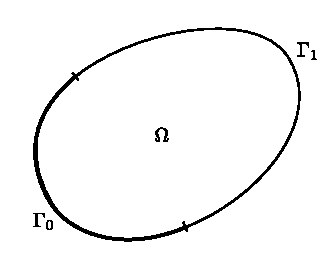
\includegraphics{vol65-figures/fig65-4.1.eps}}
  \caption{}
\end{figure}
\end{remark}

Assuming\pageoriginale  that measure of $\Gamma_0$ is positive and that $g$ is
sufficiently smooth, it can be proved that the following variant 
of~\eqref{c2:eq4.5} 
\begin{equation}
\begin{cases}
\hat{a} (u, v-u) \geq \hat{L}(v-u)\, \forall  v \in \hat{K}, \\ 
u \in \hat{K}, \tag{4.12}\label{c2:eq4.12}
\end{cases}
\end{equation}
has a unique solution.

In the proof of this result one uses the fact that $\hat{a}(v, v)$
defined a norm on $V$ which is equivalent to the norm induced by $H^1
(\Omega)$. 

\begin{exercise}\label{c2:exer4.1}%exercise 4.1 
 Prove that $a(v, v)$ defines a norm equivalent to the norm induced by
 $H^1(\Omega)$. 
\end{exercise}

\subsection{Regularity of the solution}\label{c2:ss4.2}

\begin{theorem}\label{c2:thm4.2}%theorem 4.2
 (H BREZIS [3]) Let $\Omega$ be a bounded domain of $\mathbb{R}^2$
  with a smooth boundary $\Gamma$ (or $\Omega$ is a convex, polygonal
  domain). If $L (v) = \int_\Omega fv dx$  with $f \in L^2
  (\Omega)$  then the solution $u$ of \eqref{c2:eq4.5} is in $H^2 (\Omega)$.  
\end{theorem}

\subsection{Interpretation of (4.5) as a free boundary
  problem}\label{c2:ss4.3}   

Let us recall some definitions and  results related to cones.  

\begin{definition}\label{c2:def4.1}%definition 4.1
 Let $X$ be a vector space, $C \subset X$ and $x \in C$, then $C$
 is called a cone with vertex $x$ if for all $y \in C$, $t \geq
 0$ implies $x + t (y-x) \in C$.  
\end{definition}

\begin{lemma}\label{c2:lem4.1}%lemma 4.1
 Let $H$ be a real Hilbert space, $b(\cdot, \cdot)$ a bilinear form on
 $H \times H ; \lambda$ a linear form on $H$ and $C$ a convex cone
 contained in $H$  with vertex at 0. Then every solution of  
 \begin{equation}
\begin{cases}
 b (u, v-u) \geq \lambda (v-u)\, \forall  v \in C,\\
  u \in C \tag{4.13}\label{c2:eq4.13}
\end{cases}
 \end{equation} 
 is a solution of
 \begin{equation}
\begin{cases}
b (u, v) \geq \lambda(v)\, \forall  v \in C,\\
b(u, u) = \lambda (u),\\
u \in C ,  \tag{4.14}\label{c2:eq4.14}
 \end{cases} 
 \end{equation} 
  and conversely.\pageoriginale 
\end{lemma}

\begin{exercise}\label{c2:exer4.2}%exercise 4.2
Prove Lemma~\ref{c2:lem4.1}
\end{exercise}

\begin{proposition}\label{c2:prop4.1}%proposition 4.1 
 Assume that 	
\begin{equation}
 L(v) = \int_\Omega fv dx + \int_\Gamma g \gamma v d \Gamma
 \tag{4.15}\label{c2:eq4.15}   
\end{equation}
with $f$ and $g$ sufficiently smooth. Then the solution $u$ of
\eqref{c2:eq4.5} is characterised by 
\begin{equation}
\begin{cases}
-\Delta u + u = f \text{ a.e. in }\Omega, \\
\gamma u \geq 0, \frac{\partial u}{\partial n} \geq  \text{ a.e. on
}\Gamma,\\ 
\gamma u (\frac{\partial u}{\partial n} - g) = 0 \text{ a.e. on }
\Gamma. \tag{4.16}\label{c2:eq4.16} 
\end{cases}
\end{equation}
\end{proposition} 

\begin{proof}
\begin{enumerate}
\item[(1)]First we will prove that \eqref{c2:eq4.5} implies
  \eqref{c2:eq4.16}   
\end{enumerate}
Since $K$ is a convex cone with vertex at $0$ it follows from 
Lemma~\ref{c2:lem4.1} that  
\begin{align*}
& a (u, v) \geq L(v)\, \forall  v \in K, \tag{4.17}\label{c2:eq4.17}\\
& a(u, u) = L (u). \tag{4.18}\label{c2:eq4.18}
\end{align*}
 Since $\mathscr{D} (\Omega) \subset K$ we have from \eqref{c2:eq4.17}
 that   
\begin{equation}
\int_\Omega \nabla u \cdot \nabla \phi dx + \int_\Omega
u \phi dx = \int_\Omega f \phi dx\, \forall  \phi \in \mathscr{D}
(\Omega). \tag{4.19}\label{c2:eq4.19} 
 \end{equation} 
It follows from \eqref{c2:eq4.19} that 
\begin{equation}
- \Delta u + u = f \text{ a.e. in }
\Omega. \tag{4.20}\label{c2:eq4.20}   
\end{equation}  
\end{proof}

Let $v \in K$.  Multiplying \eqref{c2:eq4.20} by $v$ and using
\textit{Green's formula} it follows that  
\begin{equation}
a(u, v) = \int_\Omega fv dx + \int_\Gamma \gamma v \frac{\partial
  u}{\partial n} d \Gamma\, \forall  v \in K. \tag{4.21}\label{c2:eq4.21}  
\end{equation}
From \eqref{c2:eq4.17} and \eqref{c2:eq4.21} we obtain 
\begin{equation}
\int_\Gamma \left(\frac{\partial u }{\partial n} - g\right) \gamma v d \Gamma
\geq 0\, \forall  v \in K. \tag{4.22}\label{c2:eq4.22} 
\end{equation}
Since\pageoriginale  the cone $\gamma K$ is  dense in $L^2_+ (\Gamma) = \{v \in
L^2(\Gamma) : v \geq 0$ \textit{a.e. on} $\Gamma \}$ it follows from
\eqref{c2:eq4.22} that  
\begin{equation}
\frac{\partial u }{\partial n} - g \geq 0 \text{ a.e. on }
\Gamma. \tag{4.23}\label{c2:eq4.23} 
\end{equation}
Taking $v=u$ in \eqref{c2:eq4.21} and using \eqref{c2:eq4.18} we
obtain  
\begin{equation}
\int_\Gamma \gamma u \left(\frac{\partial u}{\partial n}- g\right) d \Gamma =
0. \tag{4.24}\label{c2:eq4.24} 
\end{equation}

Since  $\gamma u \geq 0$ and using \eqref{c2:eq4.23} we obtain $\gamma u
\left(\dfrac{\partial u}{\partial  n}- g\right) =0 $ a.e. on
$\Gamma$. This shows that \eqref{c2:eq4.5} implies \eqref{c2:eq4.16}. 
\begin{enumerate}
\item[(1)] Let us show that \eqref{c2:eq4.16} implies
  \eqref{c2:eq4.5}. Starting from \eqref{c2:eq4.20} 
  and using Green's formula one can easily  prove \eqref{c2:eq4.17} and
  \eqref{c2:eq4.18}. These two relations in turn imply, from
  Lemma~\ref{c2:lem4.1}, that $u$ is the solution of \eqref{c2:eq4.5}.  
\end{enumerate}

\begin{remark}\label{c2:rem4.4}%remark 4.4
Similar results may be  proved for that variant \eqref{c2:eq4.12} of
\eqref{c2:eq4.5} 
(see Remark~\eqref{c2:eq4.3}.  
\end{remark}

\begin{remark}\label{c2:rem4.5}%remark 4.5
From the equivalent formulation \eqref{c2:eq4.16} of \eqref{c2:eq4.5}
it appears that the solution $u$ of \eqref{c2:eq4.5} is the solution
of a free boundary problem namely  
 
{\em Find a sufficiently smooth function $u$ and two subsets
  $\Gamma_0$ and $\Gamma_+$ such that} 
\begin{equation}
\Gamma_0  \cup \Gamma_+ = \Gamma, \Gamma_0 m \cap \Gamma_+ = \phi,
\tag{4.25}\label{c2:eq4.25} 
\end{equation}
\begin{equation}
\begin{cases}
-\Delta u+u = f \text{ in }\Omega,\\
\gamma u = 0 \text{ on }\Gamma_0, \frac{\partial u}{\partial n}\geq g \text{ on } \Gamma_0,\\
\gamma u > o ~\text{on}~ \Gamma_+, \frac{\partial u}{\partial n} = g \text{ on
} \Gamma_+.\tag{4.26}\label{c2:eq4.26} 
\end{cases}
\end{equation}
\end{remark}

\subsection{Finite element approximation of (4.5)}\label{c2:ss4.4} 

We consider\pageoriginale  in this section  the approximation of \eqref{c2:eq4.5} by
piecewise linear and piecewise quadratic finite elements. We assume
that $\Omega$ of is a bounded polygonal domain of $\mathbb{R}^2$ and
we consider a triangulation $\mathscr{C}_h$ of $\Omega$ obeying 
\eqref{c2:eq2.21}--\eqref{c2:eq2.23} (see Sec \ref{c2:ss2.5}., Chap. 2) ; we use
the notation of Sec.~\ref{c2:sss2.5.1} and \ref{c2:ss3.6} of this
chapter.  

\subsubsection{Approximation of  $V$ and $K$}\label{c2:sss4.4.1} 

The space $V=H^1(\Omega)$ may be approximated by the spaces $V^k_h$ where  
$$
V^k_h = \{v_\epsilon \in C^0 (\overline{\Omega}) : v_h |_T \in P_k,
\forall T \in \mathscr{C}_h \}, k=1, 2. 
$$
\begin{align*}
\text{ Define } \gamma_h & = \{P \in \Sigma_h \cap \Gamma \} =
\Sigma_h - \Sigma^0_h,\\ 
\gamma'_h & = \{P \in \Sigma'_h \cap \Gamma \} = \Sigma'_h -
\Sigma'^0_h,\\ 
\gamma^k_h& = \begin{cases}\gamma_h \text{ if } k=1\\ 
\gamma_h \cup \gamma'_h \text{ if } k=2 .
\end{cases}
\end{align*}
Then we approximate $K$ by 
$$
K^k_h = \{v_h \in V^k_h:v_h (P) \geq 0 \, \forall  P \in
\gamma^k_h \text{ for } k=1, 2\} . 
$$

We have then the obvious 

\begin{proposition}\label{c2:prop4.2}%proposition 4.2
For $k=1, 2$ the $K^k_h$ are closed, convex, non-empty subsets of
$V^{k}_h$ and $K^{1}_h\subset K\, \forall  h$. 
\end{proposition}

\subsubsection{The approximate problem}\label{c2:sss4.4.2} 

For $k=1, 2$ the approximate
problems are defined by  
\begin{equation*}
(P^k_{1h})
\begin{cases}
a(u^k_h, v_h-u^k_h) \geq L(v_h-u^k_h)\, \forall  v_h \in K^k_h, \\
u^k_h \in K^k_h.
\end{cases}
\end{equation*}
Then one can easily prove, 

\begin{proposition}\label{c2:prop4.3}%proposition 4.3
The problem $(P^k_{1h}) (k=1, 2)$ has a unique solution.
\end{proposition}

\begin{remark}\label{c2:rem4.6}%remark 4.6
Since\pageoriginale  $a(\cdot, \cdot)$ is symmetric, $(P^k_{1h})$ is
equivalent (See \break  
Chap.~\ref{chap1}, Sec.~\ref{c1:ss3.2}) to the quadratic programming
Problem  
$$
\min_{v_h \in K^k_h} \left[\frac{1}{2} a (v_h, v_h) -L (v_h)\right]. 
$$
\end{remark}

\begin{remark}\label{c2:rem4.7}%remark 4.7
 Using the formula of Sec.~\ref{c2:s7} One may express
 \eqref{c2:eq4.5} and the equivalent 
 quadratic problem in a form more suitable for computation.  
\end{remark}

\subsection{Convergence results. (General case)}\label{c2:ss4.5} 

\subsubsection{A density Lemma}\label{c2:sss4.5.1}
 To prove the convergence results of the following
 Sec.~\ref{c2:sss4.5.2} we shall use the following   

\begin{lemma}\label{c2:lem4.2}%lemma 4.2
Under the above assumptions on $\Omega$ we have 
$$
\overline{K \cap C^\infty (\overline{\Omega)}} = K.
$$
\end{lemma}

\begin{proof}
Since $\Gamma$ is Lipschitz continuous we have (see NECAS [1]) 
$$
H^1(\Omega) = \overline{C^\infty (\overline{\Omega)}}; 
$$
Using the standard decomposition $v = v^+ -v^-$ it follows from
Corollary~\ref{c2:cor2.1} that  
\begin{equation}
v \in  K \iff v^{-} \in H^1_0
(\omega). \tag{4.27}\label{c2:eq4.27} 
\end{equation}
\end{proof}

Since $\overline{\mathscr{D}{\Omega)}} = H^1_0 (\Omega)$ in the
$H^1(\Omega)-$ topology, it follows from \eqref{c2:eq4.27} that we
have only to prove  
\begin{equation}
\overline{\hat{K}\cap C^\infty (\Omega)} = \hat{K},
\end{equation}
where $\hat{K} = \{v \in H^1 (\Omega) , v \geq 0 $ a.e. in
$\Omega$ \}. 

Since $\Gamma$ is Lipschitz continuous, $\Omega$ has (see LIONS [2],
NECAS [1]), the so-called 1-extension property which implies  
\begin{equation}
\begin{cases}
\forall v \in H^1 (\Omega) , \exists \tilde{v} \in H^1
(\mathbb{R}^2) \text{ such that }\\ 
\tilde{v}|_\Omega = v.  \tag{4.29}\label{c2:eq4.29}
\end{cases}
\end{equation}

Let\pageoriginale  $v \in K$ and let $\tilde{v} \in H^1 (\mathbb{R}^2)$ be
an extension of $v$ obeying \eqref{c2:eq4.29}. It  follows, from $v
\geq o$ a.e. in $\Omega$ and Corollary~\ref{c2:cor2.1}, that
$|\tilde{v}|$ is also an  extension of $v$ obeying
\eqref{c2:eq4.29}. Therefore if $v \in \tilde{K}$, 
it has always an extension $\tilde{v} \geq 0$ a.e. obeying
\eqref{c2:eq4.29}. Consider such a non-negative extension $\tilde{v}$  
and a mollifying  sequence $\rho_n$ (like in Lemma~2.4 of this 
Chap.). Define $\tilde{v}_n$ by  
\begin{equation}
\tilde{v}_n = \tilde{v}* \rho_n. \tag{4.30}\label{c2:eq4.30}
\end{equation}
we have 
\begin{equation}
\begin{cases}
\tilde{v}_n \in \mathscr{D} (\mathbb{R}^2), \\
\lim \tilde{v}_n = \tilde{v} \text{ strongly in}~ H^1
(\mathbb{R}^2). \tag{4.31}\label{c2:eq4.31} 
\end{cases}
\end{equation}

From $\rho_n \geq 0$ and $\tilde{v} \geq 0$ a.e. we obtain from \eqref{c2:eq4.30} that 
\begin{equation}
\tilde{v}_n (x) \geq 0\, \forall  x \in
\mathbb{R}^2.\tag{4.32}\label{c2:eq4.32}  
\end{equation}
Define $v_n$ by 
$$
v_n = \tilde{v}_n |_{\overline{\Omega}};
$$
from \eqref{c2:eq4.31} and \eqref{c2:eq4.32} it follows that 
$$
v_n \in C^\infty (\overline{\Omega}), \lim_{n \to \infty}v_n = v
\text{ strongly }in H^1 (\Omega), v_n \geq 0 \text{ a.e.  in }
\Omega. 
$$
This proves the Lemma.

\subsubsection{Convergence theorem}\label{c2:sss4.5.2}

\begin{theorem}\label{c2:thm4.3}%theorem 4.3
Suppose that the  angles of $\mathscr{C}_h$ are uniformly bounded
below by $\theta_0 > 0$ as $h \to 0$, then  
\begin{equation}
\lim_{h \to 0} u^k_h = u \text{ strongly } in H^1(\Omega),
\tag{4.33}\label{c2:eq4.33}  
\end{equation}
where $u, u^k_h$ are respectively the solutions of (\ref{c2:eq4.5}) and
$(P^k_{1h})$  for $k=1, 2$. 
\end{theorem}

\begin{proof}
To prove \eqref{c2:eq4.33} we use Theorem~\ref{c1:thm5.2} of
Chap.~\ref{chap1}. To do this we only have 
to verify that the following two properties hold:  
\begin{enumerate}[(i)]
\item If $(v_h)_h$,\pageoriginale  $v_h \in K^k_h$, converges \textit{weakly} to
  $v$ then  $v \in K$.  
\item There exist $\chi \subset K$ and $r^k_h : \chi \to K^k_h $ such
  that $\overline{\chi}= K$ and $\displaystyle{\lim\limits_{h \to 0}} r^k_h v = v$ \textit{
    strongly } in $V$, $\forall v \in \chi$. 
\end{enumerate}
\end{proof}

\medskip 
\noindent 
\textbf{Verification of (i). }% varification of (i)
 If $k=1$, then (i) is trivially  satisfied, since $K^1_h \subset K$. 

\begin{figure}[H]
  \centering{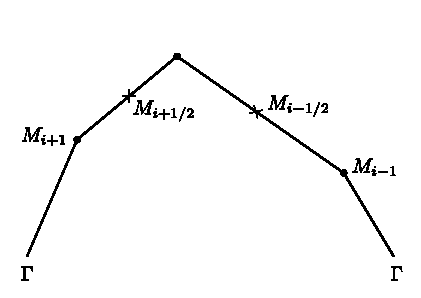
\includegraphics{vol65-figures/fig65-4.2.eps}}
  \caption{}
\end{figure}

If $k=2$, using the notation of Fig.~4.2. we consider $\phi \in
C^0 (\Gamma)$, $\phi \geq 0$, and we define $\phi_h$ by  
\begin{equation}
\phi_h = \Sigma_i \phi (M_{i+1/2}) \chi_{i+1/2}
\tag{4.34}\label{c2:eq4.34} 
\end{equation}
where $\chi_{i+1/2}$ denotes the \textit{characteristic function} of
the open segment $] M_i, M_{i+1}[$. Then  
\begin{equation}
\begin{cases}
\phi_h \geq 0 \text{ a.e. on } \Gamma ,\\
\lim\limits_{h \to 0} \parallel \phi_h - \phi\parallel_{L^\infty (\Gamma)} =
0. \tag{4.35}\label{c2:eq4.35}  
\end{cases}
\end{equation}

Let us consider a sequence $(v_h)_h$, $v_h \in K^2_h\, \forall  h$,
such that  
\begin{equation}
\lim v_h = v \text{ weakly } in V . \tag{4.36}\label{c2:eq4.36}
\end{equation}

It follows\pageoriginale  from \eqref{c2:eq4.36} (see NECAS
[\ref{k73:e1}]) that $\displaystyle{\lim\limits_{h\to 0} 
\gamma v_h = \gamma v}$ \textit{ strongly } in $L^2 (\Gamma)$. This
implies in turn that  
\begin{equation}
\lim_{h \to 0} \int_\Gamma \gamma v_h \phi_h  d \Gamma = \int_\Gamma
\gamma v \phi d \Gamma. \tag{4.37}\label{c2:eq4.37} 
\end{equation}

It follows from Simpson's rule that 
\begin{equation}
\begin{cases}
\int_\Gamma \gamma v_h \phi_h d \Gamma 
= \frac{1}{6} \Sigma_i
|\overrightarrow{M_i M_{i+1}}| \phi (M_{i+1/2})\\
\qquad [v_h (M_i) + 4v_h
  (M_{i+1/2}) + v_h (M_{i+1}) ]\geq 0\\ 
\forall v_h \in K^2_h,\, \forall  \phi \in C^0 (\Gamma) , \phi
\geq 0.\tag{4.38}\label{c2:eq4.38} 
\end{cases}
\end{equation}
We  obtain from \eqref{c2:eq4.37} and \eqref{c2:eq4.38} that 
$$
\int_\Gamma  \gamma v \phi d \Gamma \geq 0\, \forall  \phi \in C^0
(\Gamma) , \phi \geq 0, 
$$
which implies $\gamma v \geq 0$ a.e.  on $\Gamma$. 

This proves (i).

\noindent \textbf{Verification of (ii).}
From Lemma~\ref{c2:lem4.2}, it is natural to take $\chi = K \cap
C^\infty (\overline{\Omega})$. 
  Define $r^k_h ; H^1 (\Omega) \cap C^0 (\overline{\Omega}) \to V^k_h$ by 
 \begin{equation}
 \begin{cases}
r^k_h v \in  V^k_h\, \forall  v \in H^1 (\Omega) \cap C^0
(\overline{\Omega}) ,\\ 
r^k_h v(P) = v(P)\, \forall  P \in \Sigma^k_h, k=1,
2.\tag{4.39}\label{c2:eq4.39} 
 \end{cases} 
 \end{equation} 

 
On one hand, under the assumptions made on $\mathscr{C}_h$ we have
(see STRANG-FIX [\ref{k85:e1}])  
 \begin{equation}
\parallel r^k_h v-v\parallel_V \leq Ch^k \parallel v\parallel_{H^{k+1}(\omega)}\, \forall  v \in
C^\infty (\overline{\Omega}), k=1, 2.\tag{4.40}\label{c2:eq4.40} 
 \end{equation} 
 with $C$ independent of $h$ and $v$.
 
 This implies 
 \begin{equation}
\lim_{h \to 0} \parallel r^k_h v-v\parallel_v = 0\, \forall  v \in \chi, k=1,
2. \tag{4.41}\label{c2:eq4.41} 
 \end{equation} 
 On the other hand it is obvious that $r^k_h v \in K^k_h\, \forall 
 v \in K \cap C^0 (\overline{\Omega})$, so that $r^k_h v \in
 K^k_h\, \forall  v \in \chi, k=1, 2$. 
 
In conclusion, with the above $\chi$ and $r^k_h$, (ii) is satisfied. 

 \begin{remark}\label{c2:rem4.8}%remark 4.8
For error\pageoriginale  estimates in the approximation of
\eqref{c2:eq4.5} by piecewise   linear finite elements, it has been
shown by BREZZI-HAGER-RAVIART [\ref{k18:e1}] that we have  
$$
\parallel u_h-u\parallel_{H^1(\Omega)} = 0 (h),
$$
assuming reasonable smoothness hypothesis for $u$ on $\Omega$.
\end{remark} 
\subsection{Iterative methods for solving the discrete problem}\label{c2:ss4.6} 
We shall briefly describe two  types of methods which seem  to be
appropriate for solving the approximate problem  of Sec.~\ref{c2:ss4.4}. 

\subsubsection{Solution by an over-relaxation method}\label{c2:sss4.6.1} 
The approximate problem $(P^k_{1h})$ are, for $k=1, 2$, equivalent to
the quadratic programming problems described in Remark \ref{c2:rem4.6}. By virtue
of the properties of $K^k_h$ (see Sec. 4.4.1.) we can use,  for the
solution of $(P^k_{1h} )$, the over-relaxation method with projection,
which has already been used in Sec. 2.8 to  solve the approximate
obstacle problem and is described in CEA [2, Chap. 4]. From the
properties of our problem the method will converge provided $0 <
\omega < 2$.  

\subsubsection{Solution by a duality method}\label{c2:sss4.6.2} 
We first consider the \textit{continuous case.} Let us define a
Lagrangian $\mathscr{L}$ by 
\begin{equation}
\mathscr{L} (v, q) = \frac{1}{2} a(v, v) -L (v) - \int_\Gamma q \gamma
v d \Gamma. \tag{4.42}\label{c2:eq4.42} 
\end{equation} 	
and let $\lambda$ be the \textit{positive cone} of $L^2(\Gamma)$, i.e. 
$$
\Lambda = \{q \in L^2 (\Gamma) : q \geq 0 \text{ a.e. on } 
\Gamma\}. 
$$
Then we have 

\begin{theorem}\label{c2:thm4.4}%theorem 4.4
 Let  $L(v) = \int_\Omega f v dx + \int_\Gamma g \gamma v d \Gamma$
 with $f$ and $g$ sufficiently smooth. Suppose that  the solution $u$
 of \eqref{c2:eq4.5} and \eqref{c2:eq4.7} belongs to $H^2(\Omega)$;
 then $\{u, \frac{\partial u}{\partial n} -g\}$ is the unique saddle
 point of  $\mathscr{L}$ over $H^1(\Omega) \times \Lambda$. 
\end{theorem} 	

\begin{proof}
We divide\pageoriginale  the proof into two parts. In the first part we will show
that $\{u, \frac{\partial u}{\partial n}- g \}$ is a saddle point of
$\mathscr{L}$ over $H^1(\Omega) \times \lambda$ and in the second part
we will prove the uniqueness.  
\begin{enumerate}
\item[(1)] Let $p = \frac{\partial u}{\partial n} - g$. From the
  definition of a saddle point we have to prove that  
\begin{equation}
\begin{cases}
\mathscr{L}(u, q) \leq \mathscr{L} (u, p) \leq \mathscr{L} (v,p)
\forall \{v, q\} \in V \times \Lambda ,\\ 
 \{u, p\}\in V \times \Lambda . \tag{4.43}\label{c2:eq4.43}
\end{cases}
 \end{equation} 
\end{enumerate}
\end{proof}

Since $u \in H^2 (\Omega)$ we have $\frac{\partial u}{\partial n}
\in H^{1/2}(\Gamma) \subset L^2(\Gamma)$ (see LIONS -MAGENES
[1]). Then if $g$ is smooth enough we have $p =
\frac{\partial u}{\partial n} - g \in L^2(\Gamma)$. From
Proposition~\ref{c2:prop4.1} we have  
\begin{equation}
\begin{cases}
p = \frac{\partial u}{\partial n}- g \geq 0 \text{ on } \Gamma ,\\
p - \gamma u = 0 \text{ a.e. on } \Gamma. \tag{4.44}\label{c2:eq4.44}
\end{cases}
\end{equation}

This implies that we have $\{u, p\} \in H^1 (\Omega) \times
\Lambda$ and $\int_\Gamma p \cdot \gamma u d \Gamma = 0$. Since
$\gamma u \geq 0$ on $\Gamma$ we have  
\begin{equation}
\int_\Gamma q \cdot \gamma u d \Gamma \geq 0\, \forall  q \in
\Lambda .\tag{4.45}\label{c2:eq4.45} 
\end{equation}
It follows from \eqref{c2:eq4.44} and \eqref{c2:eq4.45} that
\begin{equation*}
\begin{cases}
\mathscr{L} (u, q) & = \frac{1}{2} a (u, u) = L (u)- \int_\Gamma q
\cdot \gamma u d \Gamma \leq \frac{1}{2} a (u, u) - L (u) =\\ 
& = \frac{1}{2} a (u, u) - L(u) - \int_\Gamma p \cdot \gamma u d
\Gamma = \mathscr{L} (u, p)\, \forall  q \in \Lambda   
\end{cases}
\end{equation*}
which proves the first inequality of \eqref{c2:eq4.43}. 

To prove the second inequality of \eqref{c2:eq4.43} we observe that the solution
$u^*$ of the minimisation problem  
\begin{equation}
\begin{cases}
\mathscr{L} (u^*, p) \leq \mathscr{L} (v, p)\, \forall  v \in
H^1(\Omega),\\ 
u^* \in H^1 (\Omega), \tag{4.46}\label{c2:eq4.46}
\end{cases}
\end{equation}
is unique\pageoriginale  and is actually the solution of the linear variational
equation  
\begin{equation}
\begin{cases}
a(u^*,v) = L (v) + \int_\Gamma p \gamma v d \Gamma\, \forall  v \in
H^1 (\Omega),\\ 
 u^* \in  H^1 (\Omega). \tag{4.47}\label{c2:eq4.47}
\end{cases}
\end{equation}
Since $L(v) = \int_\Omega f v dx + \int_\Gamma g \gamma v d \Gamma,
u^*$ is actually the solution of the Neumann problem  
\begin{equation}
\begin{cases}
-\Delta u^* + u^* = f \text{ in } \Omega,\\
 \frac{\partial u^*}{\partial n} =  p + g = \frac{\partial u}{
   \partial n}\text{ on } \Gamma,\tag{4.48}\label{c2:eq4.48} 
\end{cases}
\end{equation}
Since from Proposition~\ref{c2:prop4.1} we obviously have 
\begin{equation*}
\begin{cases}
-\Delta u + u = f \text{ in }\Omega,\\
 \frac{\partial u}{\partial n}= \frac{\partial u^*}{\partial n} \text{
   on }\Gamma, 
\end{cases}
\end{equation*}
it follows from the uniqueness property of the Neumann problem \eqref{c2:eq4.48}
that $u=u^*$. Using \eqref{c2:eq4.46} and $u=u^*$, we obtain the second
inequality in \eqref{c2:eq4.43}. This proves that $\{u, p\}$ is a saddle point of
$\mathscr{L}$ over $H^1(\Omega)\times \Lambda$.  

\textbf{Uniqueness.} Let $\{u^*, p^*\}$  be a saddle point of
$\mathscr{L}$ over $H^1(\Omega) \times \Lambda$. We will show that $u^*
= u, p^* =$. It follows from \eqref{c2:eq4.42} and \eqref{c2:eq4.43} that  
\begin{equation}
\int_\Gamma (p-q) \gamma u d \Gamma  \leq 0\, \forall  q \in
\Lambda. \tag{4.49}\label{c2:eq4.49} 
\end{equation}
We have similarly,
\begin{equation}
\int_\Gamma (p^*, q) \gamma u^* d \Gamma \leq 0\, \forall  q \in
\Lambda. \tag{4.50}\label{c2:eq4.50} 
\end{equation}
Taking $q = p^*$ (respectively $q=p$) in \eqref{c2:eq4.49} (respectively \eqref{c2:eq4.50})
we obtain  
\begin{equation}
\int_\Gamma  (p^* - p) \gamma (u^* - u) d \Gamma \leq 0. \tag{4.51}\label{c2:eq4.51} 
\end{equation}
It follows\pageoriginale  from the second inequality of \eqref{c2:eq4.43} that $u$ is the 
solution of  
\begin{equation}
\begin{cases}
a(u, v) = L(v) + \int_\Gamma p \cdot \gamma v d \Gamma\, \forall  v
\in H^1 (\Omega) ,\\ 
u \in H^1(\Omega). \tag{4.52}\label{c2:eq4.52}
\end{cases}
\end{equation}
ans similarly 
\begin{equation}
\begin{cases}
a(u^*, v) = L(v) + \int_\Gamma p^* \cdot \gamma v d \Gamma\, \forall  v
\in H^1 (\Omega),\\ 
 u^* \in H^1 (\Omega). \tag{4.53}\label{c2:eq4.53}
\end{cases}
\end{equation}

Taking $v = u^*-u$ (respectively  $v = u - u^*)$ in \eqref{c2:eq4.52}
(respectively \eqref{c2:eq4.53}) we obtain 
\begin{equation}
a(u^*-u,u^*-u) = \int_\Gamma  (p^*-p) \gamma (u^*-u)
d\Gamma.\tag{4.54}\label{c2:eq4.54} 
\end{equation}
Using the $V$-ellipticity of $a(\cdot, \cdot)$ it follows then from
\eqref{c2:eq4.51}--\eqref{c2:eq4.54} that $u^* =u$ and  
$$
\int_\Gamma (p^* - p) \gamma v d \Gamma = 0\, \forall  v \in H^1
(\Omega), 
$$
which implies that $p^* = p$. 

Hence $\{u, p\}$ is the unique  saddle point of $\mathscr{L}$ over
$H^1 (\Omega) \times \Lambda$. 

It follows from Theorem \ref{c2:thm4.4} that we can apply Uzawa's algorithm to
solve (\ref{c2:eq4.5}) (see CEA [\ref{k27:e2}, Chap. 5],
G.L.T. [\ref{k53:e1}, Chap.2], [\ref{k53:e2}, Chap. 4,
  Sec \ref{c2:ss3.6}]). In the present case this algorithm is written as follows:  
\begin{equation}
p^0 \in \Lambda  \text{ is arbitrarily chosen (for instance } p^0
= 0). \tag{4.55}\label{c2:eq4.55} 
\end{equation}
\textit{By induction, after knowing $p^n$ we compute $\{u^n,
  p^{n+1}\}$  by} 
\begin{align}
& \mathscr{L} (u^n, p^n) \leq \mathscr{L} (v, p^n)\, \forall  v \in
  H^1 (\Omega), u^n \in H^1 (\Omega), \tag{4.56}\label{c2:eq4.56}\\ 
& p^{n+1} = P_\Lambda  (p^n-\rho \gamma u^n), \tag{4.57}\label{c2:eq4.57}
\end{align}
where\pageoriginale  $P_\Lambda$ is \textit{projection operator} from $L^2(\Gamma)$
to $\Lambda$ in the $L^2(\Gamma)$ norm and $\rho > 0$. It follows from
\eqref{c2:eq4.56} that $u^n$ is in fact the solution of the Neumann
problem   
\begin{equation}
\begin{cases}
-\Delta u^n + u^n = f \text{ in } \Omega,\\
\frac{\partial u^n}{\partial n}| \Gamma = p^n + g. \tag{4.58}\label{c2:eq4.58}
\end{cases}
\end{equation}

The projection $P_\Lambda  $ is given by  
\begin{equation}
P_\Lambda  (q) = q^+\, \forall  q \in L^2
(\Gamma). \tag{4.59}\label{c2:eq4.59}  
\end{equation}

Since $\gamma : H^1 (\Omega) \to L^2(\Gamma)$ is a continuous linear
map we have  
\begin{equation}
\parallel \gamma v\parallel_{L^2(\Gamma)} \leq \parallel \gamma\parallel \cdot \parallel v\parallel_{H^1(\Omega)}
\forall v \in H^1(\Omega).\tag{4.60}\label{c2:eq4.60}  
\end{equation}
It follows then from CEA, G.L.T., loc. cit., that 
\begin{equation}
\lim_{n \to \infty} u^n = u \text{ strongly in}~ H^1 (\Omega),
\tag{4.61}\label{c2:eq4.61} 
\end{equation}
where $u$ is the solution of the problem \eqref{c2:eq4.5}  provided that $0 <
\rho < \frac{2}{\parallel \gamma\parallel^2}$.  

Let us give a direct proof for this convergence result. This proof
will use the characterisation \eqref{c2:eq4.5} given in
Proposition~\ref{c2:prop4.1}  
(even if $a(\cdot, \cdot)$ is not symmetric the same result follows). It will
be convenient to take \eqref{c2:eq4.56}, \eqref{c2:eq4.58} in the  following equivalent
form:  
\begin{equation}
\begin{cases}
a(u^n, v) = L (v) + \int_\Gamma p^n \gamma v d \Gamma\, \forall  v \in
H^1(\Omega), \\ 
u^n \in H^1(\Omega). \tag{4.62}\label{c2:eq4.62}
\end{cases}
\end{equation}

Let $u$ be the solution of \eqref{c2:eq4.5} and $p=\frac{\partial
  u}{\partial n}- g$. It follows from Proposition~\ref{c2:prop4.1} that  
\begin{equation}
\begin{cases}
a(u, v) = L (v) + \int_\Gamma  p \gamma v d \Gamma\, \forall  \mathscr{L}
\in H^1(\Omega),\\ 
u \in  H^1(\Omega), \tag{4.63}\label{c2:eq4.63}
\end{cases}
\end{equation}
\begin{equation}
\int_\Gamma (q-p) \gamma u d \Gamma \geq 0\, \forall  q \in \Lambda
, p \in \Lambda. \tag{4.64}\label{c2:eq4.64} 
\end{equation}\pageoriginale 
Relation \eqref{c2:eq4.64} can also be written as 
$$
\int_\Gamma (q-p) (p-\rho \gamma u-p) d \Gamma \leq 0\, \forall   q
\in \Lambda , \rho > 0.  
$$
which is classically equivalent to 
\begin{equation}
p = P_\Lambda  (p - \rho \gamma u). \tag{4.65}\label{c2:eq4.65}
\end{equation}

Let  consider: 
$$
\overline{u}^n = u^n -u, \overline{p}^n = p^n - p.
$$
Since $P_\Lambda $ is a contraction , we have from \eqref{c2:eq4.57}
and \eqref{c2:eq4.65}   
\begin{equation}
\parallel \overline{p}^{n + 1}\parallel_{L^2(\Gamma)} \leq \parallel \overline{p}^n - \rho
\gamma \overline{u}^n \parallel_{L^2(\Gamma)}.\tag{4.66}\label{c2:eq4.66} 
\end{equation}
It follows from \eqref{c2:eq4.66} that 
\begin{equation}
\parallel \overline{p}^n \parallel_{L^2(\Gamma)}^2
\parallel \overline{p}^{n+1}\parallel_{L^2(\Gamma)} \geq 2 \rho \int_\Gamma \gamma
\overline{u}^n \overline{p}^n d \Gamma -\rho^2 \parallel \gamma
\overline{u}^n\parallel^2_{L^2(\Gamma)}. \tag{4.67}\label{c2:eq4.67} 
\end{equation}

Taking $v = \overline{u}^n$ \eqref{c2:eq4.62} and \eqref{c2:eq4.63} we obtain 
\begin{equation}
a(\overline{u}^n, \overline{u}^n) = \int_\Gamma \overline{p}^n \gamma
\overline{u}^n d \Gamma. \tag{4.68}\label{c2:eq4.68} 
\end{equation}
It follows then from \eqref{c2:eq4.67} and \eqref{c2:eq4.68} that  
\begin{equation}
\parallel \overline{p}^n\parallel^2_{L^2(\Gamma)} -
\parallel \overline{p}^{n+1}\parallel^2_{L^2(\Gamma)} \geq \rho (2-\rho \parallel \gamma\parallel^2
) \parallel \overline{u}^n\parallel^2_{H^1(\Omega)}.\tag{4.69}\label{c2:eq4.69} 
\end{equation}
If $0 < \rho < \frac{2}{\parallel \gamma\parallel^2}$ we observe that the sequence
$\{\parallel \overline{p}^n\parallel^2_{L^2 (\Gamma)}\}_n$ is decreasing and hence
converges. Therefore we have  
$$
\lim_{n \to \infty}(\parallel \overline{p}^n\parallel^2_{L^2(\Gamma)} -
\parallel \overline{p}^{n+1}\parallel^2 _{L^2(\Gamma)}) = 0  
$$
so that 
$$
\lim_{n \to \infty}\parallel \overline{u}^n\parallel_{H^1(\Omega)} = 0. 
$$

Since\pageoriginale  $\overline{u}^n = u^n - u$, we have proved the convergence.  

Similarly  we can solve the approximate problem $(P^k_{1h})$, $k = 1,
2$,  using the discrete version of algorithm
\eqref{c2:eq4.55}--\eqref{c2:eq4.57}. 
We shall limit ourselves to $k=1$, since the extension here to $k=2$
is almost trivial. 

We use here the notations of Sec.~\ref{c2:ss4.1}. Assume that $\gamma_h =
\Sigma_h - \Sigma^0_h$ has been ordered. 

Let  $\gamma_h = \{M_i\}_i$.

We approximate $\Lambda $ and $\mathscr{L}$ by
$$
\Lambda^1_h = \{q_h : q_h = \{q_i\}_i, q_i \geq 0\} \text{ and } 
$$
\begin{equation}
\begin{cases}
\mathscr{L}^1_h (v_h, q_h) = & \frac {1}{2} a (v_h, v_h) -L (v_h)\\
&-\frac{1}{2} \Sigma_i |M_i M_{i+1} | [q_i v_h (M_i) + q_{i+1} v_h
  (M_{i+1})]. 
\end{cases}
\end{equation}

We can prove that $\mathscr{L}^1_h$ has a unique saddle point $\{u_h,
p_h\}$ where $p_h$ is a F. John-Kuhn-Tucker vector for $(P^1_{1h})$
over $V^1_h \times \Lambda^1_h$ and $u_h$ is precisely the solution of
$(P^1_{1h})$. The discrete analogue of
\eqref{c2:eq4.55}--\eqref{c2:eq4.57} is then  
\begin{equation}
p^0_h \in \Lambda^1_h. \tag{4.71}\label{c2:eq4.71}
\end{equation}
\begin{equation}
\begin{cases}
\mathscr{L}^1_h (u^n_h, p^n_h) \leq \mathscr{L}^1_h (v_h, p^n_h)
\forall v_h \in V^1_h, \\ 
u^n_h \in V^1_h.\tag{4.72}\label{c2:eq4.72}
\end{cases}
\end{equation}
\begin{equation}
p^{n+1}_i = [p^n_i - \rho u^n_h (M_i)]^+\, \forall  i, \rho
>0. \tag{4.73}\label{c2:eq4.73}
\end{equation}

One can prove that if $0 < \rho < \beta$, $\beta$ small enough, then
$\displaystyle{\lim\limits_{n \to +\infty}} u^n_h = u_h$ where $u_h$ is  the solution of
$(P^1_{1h})$. One may find in G.L.T. [2, Chap.4] numerical
applications of the above iterative methods for piecewise linear and
piecewise quadratic approximations of \eqref{c2:eq4.5}. 

\begin{exercise}\label{c2:exer4.3}%exercise4.3
Extend  the above considerations to $(P^2_{1h})$.
\end{exercise}

\section[An Example of EVI  of The Second Kind:...]{An Example of EVI
  of The Second Kind: A Simplified Friction Problem}\label{c2:s5} 

\subsection{The continuous problem. Existence and Uniqueness
  results}\label{c2:ss5.1} \pageoriginale 

Let $\Omega$ be a bounded domain of $\mathbb{R}^2$ with a smooth
boundary $\Gamma = \partial \Omega$. Using the same notations as in
Sec.~\ref{c2:s4} we define 
\begin{equation}
V = h^1 (\Omega), \tag{5.1}\label{c2:eq5.1}
\end{equation}
\begin{align}
& a (u, v) = \int_\Omega \nabla u  \cdot \nabla v dx +
  \int_\Omega u v dx.\tag{5.2}\label{c2:eq5.2}\\ 
& L(v) = <f, v> , f \in V^*,\tag{5.3}\label{c2:eq5.3}\\
& j(v) = g \int_\Gamma | \gamma v | d \Gamma, \text{ where } g
  >0. \tag{5.4}\label{c2:eq5.4} 
\end{align}

We have then the following 

\begin{theorem}%theorem 5.1
 The variational inequality
\begin{equation}
\begin{cases}
a(u, v-u) + j (v) - j (u) \geq  L (v-u)\, \forall  v \in V.\\ 
u \in V.\tag{5.5}\label{c2:eq5.5}
\end{cases}
\end{equation}
has a unique solution.
\end{theorem}

\begin{proof}
In order to apply Theorem~\ref{c2:thm4.1} of Chap.~\ref{chap1}, it is
enough to verify that $j(\cdot)$ is convex, proper and l.s.c. Actually
$j(\cdot)$ is a seminorm on $V$. Therefore using Schwartz inequality
in $L^2(\Gamma)$ and the fact that $\gamma \in \mathscr{L}
(H^1(\Omega)$, $L^2 
(\Gamma))$ we have  
\begin{equation}
|j(u) - j(v)| \leq | j(u-v) | \leq g (meas \cdot
\Gamma)^{1/2}\parallel \gamma(v-u)\parallel_{L^2(\Gamma)}\leq C \parallel  u - v\parallel_V,
\tag{5.6}\label{c2:eq5.6} 
\end{equation}
for some constant $C$.
\end{proof}

Hence $j(\cdot)$ is Lipschitz continuous on $V$, so that $J(\cdot)$ is
l.s.c ; $j(\cdot)$  is obviously convex and proper. Hence the Theorem
is proved. 

\begin{remark}\label{c2:rem5.1}%remark 5.1
If $g=0$, it is easy to prove that \eqref{c2:eq5.5}  reduce to the
variational equation   
\begin{equation*}
\begin{cases}
a(u, v) = L(v)\, \forall  v \in V,\\
 u \in V.
\end{cases}
\end{equation*}
This is related  to the variational formulation of the
\textit{Neumann} problem. 
\end{remark}

\begin{remark}\label{c2:rem5.2}%remark 5.2
 Since\pageoriginale  $a(\cdot, \cdot)$ is symmetric,. the solution $u$ of a \eqref{c2:eq5.5} is
 characterised, using Lemma~\ref{c1:lem4.1} of Chap.~\ref{chap1}, as
 the unique  solution of  the minimization problem  
 \begin{equation}
\begin{cases}
J(u) \leq J(v) ,\, \forall  v \in V, \\
u \in V, \tag{5.7}\label{c2:eq5.7}
\end{cases}
 \end{equation} 
 where $J(v) = \dfrac{1}{2} a (v, v) + j (v) -L(v)$. 
\end{remark}

\begin{remark}\label{c2:rem5.3}%remark 5.3
The problem \eqref{c2:eq5.5} (and \eqref{c2:eq5.7}) is the  simplified version of a {\em
  friction} problem occurring in {\em elasticity.} For  this types of
problems we refer to DUVAUTLIONS [1]and the bibliography therein. 
 \end{remark} 

 \begin{exercise}\label{c2:exer5.1}%exercise 5.1
 Let us denote by $u_g$ the solution of \eqref{c2:eq5.5}. Then prove
 that  
 $$
 \lim_{g \to + \infty}  u_g = \hat{U}\text{ strongly in}~ H^1(\Omega),  
 $$
 where $\hat{u}$ is the unique solution of 
\begin{equation*}
\begin{cases}
a(\hat{u}, v) = L (v)\, \forall  v \in H^1_0 (\omega),\\ 
 \hat{u}\in H^1_0 (\Omega).
 \end{cases}
 \end{equation*}
  \end{exercise} 
  
 \subsection{Regularity of the solution}\label{c2:ss5.2}
 
 \begin{theorem}\label{c2:thm5.2}%theorem 5.2
 (H. BREZIS [\ref{k14:e3}]). If $\Omega$ is a bounded domain  with a smooth
   boundary and if $L(v) = \int_\Omega f  v dx$ with $f \in
   L^2(\Omega)$, then the solution $u$ of \eqref{c2:eq5.5} is in $H^2(\Omega)$. 
 \end{theorem} 
 
 \subsection{Existence of a multiplier}\label{c2:ss5.3} 
Let us define $\Lambda$ by 
 $$
\Lambda  = \{\mu \in L^2 (\Gamma) : |\mu (x)| \leq 1  \text{
  a. e. in }\Gamma \}. 
 $$
Then we have 
\begin{theorem}\label{c2:thm5.3}%theorem 5.3
 The solution $u$ of \eqref{c2:eq5.5} is characterised by the
 existence of $\lambda$ such that  
 \begin{equation}
\begin{cases}
a(u, v) + g \int_\Gamma \lambda \gamma v d \Gamma = L(v)\, \forall  v
\in V,\\ 
 u \in V, \tag{5.8}\label{c2:eq5.8}
\end{cases}
 \end{equation} 
 \begin{equation}
\begin{cases}
\lambda \in \Lambda , \\
 \lambda \gamma u = |\gamma u|  \text{ a. e. in
 }\Gamma.\tag{5.9}\label{c2:eq5.9}  
\end{cases}
 \end{equation}\pageoriginale 
 \end{theorem} 
 
 \begin{proof}
We will prove first that \eqref{c2:eq5.5} implies  \eqref{c2:eq5.8} 
and \eqref{c2:eq5.9}. 

Taking $v=0$ and $v =2u$ in \eqref{c2:eq5.5} we have 
  \begin{equation}
a(u, u) + j (u) = L(u). \tag{5.10}\label{c2:eq5.10}
  \end{equation}  
It follows  then from \eqref{c2:eq5.5}, \eqref{c2:eq5.10} that  
$$
L(v) -a(u, v) \leq j(v)\, \forall  v \in V,
$$
which implies 
\begin{equation}
|L(v) -a(u, v) | \leq j(v) = g \int_\Gamma |\gamma v |d \Gamma\, \forall 
v \in V. \tag{5.11}\label{c2:eq5.11} 
\end{equation}  
 \end{proof} 
 
We have $H^1(\Omega) = H^1_0 (\Omega) \oplus [H^1_0 (\Omega)]^\perp$
where $[H^1_0 (\Omega)]^\perp$ is the orthogonal complement of $H^1_0
(\Omega)$in $H^1(\Omega)$. 
  
Since $\gamma : [H^1_0 (\Omega)]^\perp \to H^{1/2}(\Gamma)$ is an
isomorphism, it follows from \eqref{c2:eq5.11} that  
\begin{equation}
L(v) -a(u, v) = \ell (\gamma v)\, \forall  v \in V,
\tag{5.12}\label{c2:eq5.12}  
\end{equation}
where $\ell(\cdot)$  is a continuous linear functional on
$H^{1/2}(\Gamma)$. It follows then from \eqref{c2:eq5.11},
\eqref{c2:eq5.12} that   
\begin{equation}
|\ell (\mu) | \leq g \parallel \mu \parallel_{L^1(\Gamma)}\, \forall  \mu \in
H^{1/2} (\Gamma). \tag{5.13}\label{c2:eq5.13} 
\end{equation}

Since $H^{1/2}(\Gamma) \subset L^1 (\Gamma)$ it follows from
\eqref{c2:eq5.13} that, we can apply to $\ell(\cdot)$, the Hanh-Banach
Theorem (see for instance YOSIDA [1]) to obtain the existence of
$\lambda \in L^\infty (\Gamma)$, $| \lambda (x) | \leq 1$ a.e. in
$\Gamma$ such that  
\begin{equation}
\ell(\mu) = g \int_\Gamma \lambda \mu d \Gamma\, \forall  \mu \in
H^{1/2} (\Gamma). \tag{5.14}\label{c2:eq5.14} 
\end{equation}
Therefore\pageoriginale  it follows from \eqref{c2:eq5.12} and \eqref{c2:eq5.14} that 
$$
a(u, v) + g \int_\Gamma \lambda \gamma v d \Gamma = L (v)\, \forall  v
\in V , 
$$
which proves \eqref{c2:eq5.8}.
 
 Taking $v=u$ in \eqref{c2:eq5.8} we obtain 
 $$
 a(u, u) + g \int_\Gamma  \lambda \gamma u d \Gamma = L(u). 
 $$
 Using \eqref{c2:eq5.10} and the above equation we obtain 
 \begin{equation}
\int_\Gamma (|\gamma u| - \lambda \gamma u) d \Gamma = 0.\tag{5.15}\label{c2:eq5.15} 
 \end{equation} 
 Since $|\lambda|\leq 1$ a.e. we have 
 \begin{equation}
|\gamma u| - \lambda \gamma u \geq 0 ~\text{a.e.}~ \tag{5.16}\label{c2:eq5.16} 
 \end{equation} 
 It follows from \eqref{c2:eq5.15} and \eqref{c2:eq5.16} that 
 $$
 |\gamma u | = \lambda \gamma u~ a.e. 
 $$
 This completes the proof of \eqref{c2:eq5.8} and \eqref{c2:eq5.9}. 
Assuming \eqref{c2:eq5.8} and \eqref{c2:eq5.9}
 we will show that \eqref{c2:eq5.5} holds. 
 
 Let $\{u, \lambda\}$ be a solution of \eqref{c2:eq5.8},
 \eqref{c2:eq5.9}.  It follows from \eqref{c2:eq5.8} that 
 $$
 a(u, v-u) +g \int_\Gamma \lambda \gamma (v - u) d\Gamma  = L (v - u)
\, \forall  v \in V,  
 $$
 which can also be written as 
 \begin{equation}
a(u, v-u) + g \int_\Gamma \lambda \gamma v d \Gamma - g \int_\Gamma
\lambda \gamma u d \Gamma = L(v-u)\, \forall  v \in
V. \tag{5.17}\label{c2:eq5.17}  
 \end{equation} 
 From \eqref{c2:eq5.9} and \eqref{c2:eq5.17} we obtain 
 \begin{equation}
a(u, v-u) +g \int_\Gamma  \lambda \gamma v d \Gamma - g \int_\Gamma
|\gamma u| d \Gamma = L (v-u)\, \forall  v \in V. \tag{5.18}\label{c2:eq5.18} 
 \end{equation} 
 But since $\lambda \gamma v \leq | \gamma v |$ a.e. in $\Gamma$, it
 follows from \eqref{c2:eq5.18} that  
 $$
 a(u, v-u) + j (v) - j(u) \geq  L(v-u)\, \forall  v \in V. 
 $$\pageoriginale 
 This proves the characterization.

 \begin{remark}\label{c2:rem5.4}%remark 5.4
 Assuming that 
 $$
 L(v) = \int_\Omega f_0 v dx + \int_\Gamma  f_1 \gamma v d\Gamma,
 $$  
 with $f_0$, $f_1$ sufficiently smooth, we can express \eqref{c2:eq5.8} by 
\begin{equation}
\begin{cases}
-\Delta u+u = f_0 \text{ in } \Omega,\\
\frac{\partial u}{\partial n}+ g \lambda = f_1  \text{ a. e. on }
\Gamma. \tag{5.19}\label{c2:eq5.19} 
\end{cases}
 \end{equation}
 It follows from \eqref{c2:eq5.19} that $\lambda$ is unique.
 \end{remark}  
 
 \begin{exercise}\label{c2:exer5.2}%exercise 5.2 
Prove that $\lambda$ is unique $\forall L \in V^*$. 
  \end{exercise}  

 \subsection{Finite element approximation of (5.5)}\label{c2:ss5.4}
  Let $\Omega$ be a bounded domain of $\mathbb{R}^2$. The notation
  used here is mostly the same as in Sec.~\ref{c2:ss4.4} of this Chapter.  
\subsubsection{Approximation of $V$}\label{c2:sss5.4.1}
We use the piecewise  linear and
piecewise quadratic approximations of $V = H^1(\Omega)$ described in
Section~\ref{c2:sss4.4.1} of this chapter. 
\subsubsection{Approximation of$j (\cdot)$}\label{c2:sss5.4.2} 
We use the notation of  Figure~4.2. Then we approximate $j(\cdot)$ by  
\begin{equation}
j^1_h(v_h) = \frac{g}{2} \sum_i |\overrightarrow{M_i M}_{i+1}|
(|\gamma v_h(M_i)  | + |\gamma v_h )M_{i+1})|)\, \forall  v_h \in
V^1_h, \tag{5.20}\label{c2:eq5.20}  
\end{equation} 
\begin{equation}
\begin{cases}
j^2_h (v_h) & = \frac{g}{6}\sum_i |\overrightarrow{M_i M}_{i+1}| (
|\gamma v_h (M_i) |+4 | \gamma v_h (M_{i+1/2}| \\ 
 & + |\gamma v_h (M_{i+1}) |)\, \forall  v_h \in
V^2_h. \tag{5.21}\label{c2:eq5.21}  
\end{cases}
 \end{equation} 
 In \eqref{c2:eq5.20} and \eqref{c2:eq5.21} we have $M_i \in
 \gamma_h$ and $M_{i+1/2} \in \gamma'_h$. 

 \begin{remark}\label{c2:rem5.5}%remark 5.5
 Clearly \eqref{c2:eq5.20}, \eqref{c2:eq5.21} are respectively
 obtained from $j(\cdot)$ by  using Trapezoidal and Simpson's
 numerical integration formulae.  
 \end{remark} 

\subsubsection{The approximate problem}\label{c2:sss5.4.3}

For $k=1$, $2$\pageoriginale  the problem \eqref{c2:eq5.5} is approximated by 
\begin{equation*}
(P^k_{2h})
\begin{cases}
a (u^k_n, v_h - u^k_h) + j^k_h (v_h)- j^k_h (u^k_h) \geq L (v_h -
u^k_h)\, \forall  v_h \in V_h,\\ 
u^k_h \in V^k_h.
\end{cases}
\end{equation*}
Then,
\begin{proposition}\label{c2:prop5.1} %proposition 5.1
The problem $(P^k_{2h})$ has a unique solution.
\end{proposition}

\begin{remark}\label{c2:rem5.6}%remark 5.6
Since $a(\cdot , \cdot)$ is symmetric, $(P^k_{2h})$ is equivalent to
the  nonlinear programing problem  
\begin{equation}
\min_{v_h \in V^k_h} \left[\frac{1}{2} a (v_h, v_h) +  j^k_h (v_h) - L
  (v_h)\right]. \tag{5.22}\label{c2:eq5.22} 
\end{equation}
\end{remark}

\begin{remark}\label{c2:rem5.7}% remark 5. 7
Using \eqref{c2:eq5.20}, \eqref{c2:eq5.21} and
\eqref{c2:eq7.1}--\eqref{c2:eq7.4} 
of Section~\ref{c2:s7} of this chapter, we may express $(P^k_{2h})$
and \eqref{c2:eq5.22} in a form more suitable for computations. 
\end{remark}

\subsection{Convergence results}\label{c2:ss5.5} %5.5 convergence results.

\begin{theorem}\label{c2:thm5.4}% theorem 5. 4
Suppose that the angles of $\mathscr{C}_h$ are uniformly bounded below
by $\theta > 0$ as $ h \to 0$, then  
\begin{equation} 
\lim_{h \to 0} u^k_h = u \text{ strongly in } H^1 (\Omega),
\tag{5.23}\label{c2:eq5.23}
\end{equation}
where $u$ and $u^k_h$ are respectively the solutions of \eqref{c2:eq5.5} and
$(P^k_{2h})$ for $k=1,2$. 
\end{theorem}

\begin{proof}
To prove \eqref{c2:eq5.23} it is enough to verify the following (see
Theorem~\ref{c1:eq6.3} of Chapter~\ref{chap1}) 
\begin{enumerate}[(i)]
\item There exists $U \subset V$, $\overline{U} = V$ and
\begin{align*}
& r^k_h : U \to V^k_h \text{ such that }\\
& \lim_{h \to 0} r^k_h v = v \text{ strongly in } V\, \forall  v \in
  U, 
\end{align*}
\item If $V_h \to v$ {\em weakly } in $V$ then 
$$
\liminf_{h \to 0 }  j^k_h (v_h) \geq j (v).
$$
\item $\lim\limits_{h \to 0} j^k_h (r^k_h v) = j(v)\, \forall  v \in
  U$.\pageoriginale  
\end{enumerate} 
\end{proof}

\medskip
\noindent 
\textbf{Verification of (i). }% verification i
 Since $\Gamma$ is Lipschitz continuous we have (see NECAS [\ref{k73:e1}])   
\begin{equation}
\overline{C^\infty (\overline{\Omega})} = H^1
(\Omega). \tag{5.24}\label{c2:eq5.24} 
\end{equation}


Therefore it is natural to take $U= C^\infty
(\overline{\Omega})$. Define $r^k_h$ by \eqref{c2:eq4.39} if Theorem \ref{c2:thm4.3},
chap.~\ref{chap2}; under the above assumption on $\mathscr{C}_h$ it follows from
STRANG-FIX [\ref{k85:e1}] that  
\begin{equation}
\parallel r^k_h v-v \parallel_V \leq C h^k \parallel  v \parallel_{H^{k +1} (\Omega)}\, \forall  v
\in V, \tag{5.25}\label{c2:eq5.25} 
\end{equation}
 where $C$ is a constant independent of $h$ and $v$. This implies (i).
 
\medskip
\noindent 
\textbf{Verification of (ii). }% verification ii
 \begin{enumerate}
\item [(1)]{\em Case $k = 1$.} We use again the notation of Figure
  4. 2. Since the trace of $v_h$ restricted to $[M_i, M_{i+1}]$ is
  affine it follows that  
\begin{equation}
\begin{cases}
y v_h (M) = \frac{1}{|M_i M_{i + 1}|} (|\overrightarrow{M M}_{i + 1}|
\gamma v_h (M_i) + |\overrightarrow{MM}_i| \gamma v_h (M_{i +1})),\\ 
\forall v_h \in V^1_h,\, \forall  M \in [M_i, M_{i +1}].
\end{cases}
\tag{5.26}\label{c2:eq5.26}
\end{equation}
 \end{enumerate}
 $$
 \text{ Since } \frac{|\overrightarrow{MM}_{i +1}|}{|
   \overrightarrow{M_i M}_{i + 1}|} + \frac{|\overrightarrow{M
     M}_i|}{|\overrightarrow{M_i M}_{i + 1}|} =1 , 
 $$
 the convexity of $\xi \to |\xi|$ implies
 \begin{equation*}
\begin{cases}
|\gamma v_h (M)| \leq \frac{1}{|\overrightarrow{M_i M}_{i + 1}|}
(|\overrightarrow{M M}_{i + 1}||\gamma v_h (M_i)|\\ 
 \quad + |\overrightarrow{M_i M}|~ |\gamma v_h (M_{i+1})|)\, \forall  v_h
 \in V^1_h,\, \forall  M \in [M_i, M_{i+1}]. 
\end{cases}
\tag{5.27}\label{c2:eq5.27}
 \end{equation*} 
 Interesting \eqref{c2:eq5.27} on $\widehat{M_i M}_{i + 1}$ we obtain 
 $$
 \int_{\widehat{M_i M_{i +1}}} | \gamma v_h | d \Gamma \leq \dfrac{
   |\overrightarrow{M_i M}_{i +1}|}{2} (|\gamma v_h (M_i)| + |\gamma
 v_h (M_{i +1})|) 
 $$
 which implies that $\forall v_h \in V^1_h$ we have
 \begin{equation*}
\begin{cases}
j(v_h) = g \int_\Gamma | \gamma v_h | d \Gamma & = g \sum\limits_i
\int_{\widehat{ M_i M_{i +1}}} | \gamma v_h | d \Gamma \leq\\ 
& \leq \frac{g}{2} \sum\limits_i |\overrightarrow{M_i M}_{i + 1}|
(|\gamma v_h (M_i)| + |\gamma v_h (M_{i + 1})|)\\
& = j^1_h (v_h). 
\end{cases}
 \end{equation*}\pageoriginale  
  Thus we have proved 
  \begin{equation}
j(v_h) \leq j^1_h (v_h)\, \forall  v_h \in V^1_h. \tag{5.28}\label{c2:eq5.28} 
  \end{equation}  

  Let $v_h \to v$ \textit{weakly} in $V$. Then $\lim\limits_{h \to 0}
  \gamma (v_h) = \gamma (v)$ \textit{strongly} in $L^2 (\Gamma)$,
  which implies  
\begin{equation}
\lim_{h \to 0} j(v_h) = j (v). \tag{5.29}\label{c2:eq5.29} 
\end{equation}  
It follows then from \eqref{c2:eq5.28} and \eqref{c2:eq5.29} that
$\lim\limits_{h \to 0} \inf j^1_h (v_h) \geq j (v)$, which proves (ii)
if $k=1$.   
\begin{enumerate}
\item[(2)] {\em case $k = 2$.} Let us define $M_{i + 1/6'} M_{i + 5/6}$
  by (see Figure 5.1) 
$$
\overrightarrow{M_i M}_{i +1 / 6} = \frac{1}{6} \overrightarrow{M_i
  M}_{i +1}, \overrightarrow{M_i M}_{i +5 / 6} = \frac{5}{6}
\overrightarrow{M_i M}_{i +1}. 
$$ 
\end{enumerate}

\setcounter{figure}{0}
\begin{figure}[H]
  \centering{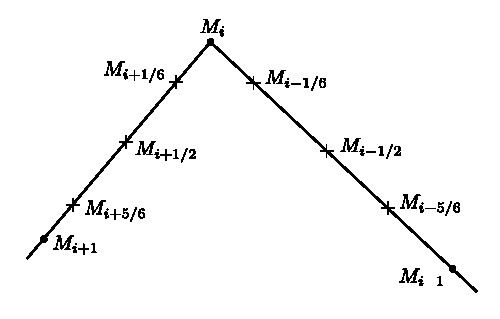
\includegraphics{vol65-figures/fig65-5.1.eps}}
  \caption{}
\end{figure}

Then we\pageoriginale  define $q_h : C^0 (\Gamma) + L^\infty (\Gamma)$ by 
\begin{equation}
\begin{cases}
q_h (\mu) = \sum\limits_{M_i \in \gamma_h} \mu (m_i) X_i +
\sum\limits_{M_\frac{i + 1}{2} {\in \gamma'_h}}, \mu(M_{i +1/ 2}) X_{i
  + 1/ 2}\\ 
\forall \mu \in C^0 (\Gamma).
\end{cases}
\tag{5.30}\label{c2:eq5.30}
\end{equation}
where $X_i$ (\textit{ respectively } $ X_{i + 1 / 2}$) is the
\textit{characteristic} function of \break $M_{i- 6}M_i M_{i +1/6}$
(respectively $\widehat{M_{i +1/6}M_{i + 5/6}}$). We have then the
following obvious properties : 
\begin{align}
& \lim_{h \to 0} q_h (\mu) = \mu \text{ strongly in } L^\infty
  (\Gamma) ~\, \forall  \mu \in C^\circ (\Gamma), \tag{5.31}\label{c2:eq5.31}\\ 
& j^2_h (v_h) = g \int_\Gamma |q_h \gamma v_h | d \Gamma = g \parallel  q_h
  \gamma v_h \parallel_{L ^1 (\Gamma)}~\, \forall  v_h \in V^2_h,
  \tag{5.32}\label{c2:eq5.32}\\ 
& C_1 \parallel  \gamma v_h \parallel_{L^2 (\Gamma ) } \leq \parallel  q_h \gamma v_h \parallel_{L^2
    (\Gamma)} \leq C_2 \parallel  \gamma v_h \parallel_{L^2 (\Gamma)} ~\, \forall  v_h
  \in V^2_h, \tag{5.33}\label{c2:eq5.33} 
\end{align}
where in \eqref{c2:eq5.33}, $C_1$ and $C_2$ are positive constants
independent of $v_h$, $h$ and $\Gamma$ (values for $C_1$ and $C_2$ may
be found in G. L. T. [2, Chap. 4]). 

Now taking $\mu \in C^0 (\Gamma)$, we define $s_h (\mu)$ by 
\begin{equation}
\begin{cases}
s_h (\mu) \in L^\infty (\Omega),\\
s_h (\mu)|_{] M_i , M_{i + 1}[} = \mu (M_{i + 1/ 2}).
\end{cases}
\tag{5.34}\label{c2:eq5.34}
\end{equation}
Then 
\begin{equation}
\lim_{h \to 0} s_h (\mu) = \mu \text{ strongly in } L^\infty (\gamma),
\tag{5.35}\label{c2:eq5.35} 
\end{equation}
and from Simpson's integration formula we have 
\begin{equation}
\int_\Gamma s_h (\mu ) q_h \gamma_h v_h d \Gamma = \int_\Gamma s_h
(\mu) \gamma v_h d \Gamma ~\, \forall  \mu \in C^\circ (\Gamma),
\forall v_h \in V^2_h. \tag{5.36}\label{c2:eq5.36} 
\end{equation}

Let $v_h \to v$ weakly in $V$, $v_h \in V^2_h\, \forall  h$, then  
\begin{equation}
\lim_{h \to 0} \gamma v_h = \gamma v \text{ strongly in } L^2
(\Gamma). \tag{5.37}\label{c2:eq5.37} 
\end{equation}

On the\pageoriginale  one hand it follows from \eqref{c2:eq5.33} that 
\begin{equation}
\parallel q_h \gamma v_h \parallel_{L^2 (\Gamma )} \leq C,\tag{5.38}\label{c2:eq5.38}
\end{equation}
where $C$ is independent of $h$.

On the other hand \eqref{c2:eq5.31},
\eqref{c2:eq5.35}--\eqref{c2:eq5.38} imply that  
\begin{equation}
\lim_{h \to 0} \int_\Gamma s_h (\mu) q_h \gamma v_h d \Gamma =
\int_\Gamma \mu \gamma v d \Gamma ~\, \forall  \mu \in C^0
(\Gamma). \tag{5.39}\label{c2:eq5.39} 
\end{equation}
In turn \eqref{c2:eq5.38} and \eqref{c2:eq5.39} imply that  
\begin{equation}
\lim_{h \to 0} q_h \gamma v_h = v \text{ weakly in } L^2 (\Gamma)
. \tag{5.40}\label{c2:eq5.40} 
\end{equation}

Since the functional $\mu \to \parallel  \mu \parallel_{L ^ 1(\Gamma)}$ is convex and
continuous on $L^1 (\Gamma)$ it follows from \eqref{c2:eq5.40} that  
\begin{equation}
\liminf_{ h \to 0 } \parallel  q_h \gamma v_h \parallel_{L^1 (\Gamma)} \geq \parallel  \gamma
v \parallel_{L^1 (\Gamma)} \tag{5.41}\label{c2:eq5.41} 
\end{equation}

Combining \eqref{c2:eq5.41} with \eqref{c2:eq5.32} we obtain
$\liminf\limits_{h \to 0}  j^2_h (v_h) \geq j (v)$ which proves (ii)
when $k = 2$.

\medskip
\noindent 
\textbf{Verification of (iii). }% verification iii
Let $v \in U = C^\infty (\overline{\Omega})$. From \eqref{c2:eq5.25} and
from the uniform continuity of $\gamma v$ on $\Gamma $ it follows
almost immediately that  
$$
\lim_{h \to 0} j^k_h (r^k_h v_h) = j(v), k=1, 2.
$$

Since the condition (i), (ii) and (iii) are satisfied the strong
convergence of $u_h$ to $u$ follows from the Theorem~\ref{c1:thm6.2}
of Chap.~\ref{chap1}.  

\begin{remark}\label{c2:rem5.8}%remark 5.8
It is proved in G. L. T. [2, Chap. 4] that $v_h \to v$ {\em weakly} in
$v, v/2 \in V^k_h$, implies $\displaystyle{\lim\limits_{h \to 0}} j^k_h (v_h) = j(v),
k=1, 2$.  
\end{remark}

Since the proof of this result is rather technical we have used in
these notes a simpler approach from which it follows that  
$$
\liminf_{h \to 0} j^k_h (v_h) \geq j(v), k=1, 2.
$$
As we have seen before this result was sufficient for proving 
Theorem~\ref{c2:thm5.4}. 

\subsection{Iterative methods for solving
  $(P^k_{2h})$.}\label{c2:ss5.6}% 5. 6 

In this\pageoriginale   section we briefly describe some iterative methods which may
be useful for solving the approximate problems $(P^k_{2h})$. 

\subsubsection{Solution of $(P^k_{2h})$ by relaxation
  methods}\label{c2:sss5.6.1}% 5. 6. 1   
It follows from \eqref{c2:eq5.20}--\eqref{c2:eq5.22} (see
Remark~\ref{c2:rem5.6}) that $(P^k_{2h}), k=1, 2$, are particular
cases of  
\begin{equation}
\min_{v \in \mathbb{R}^N} f (v),\tag{5.42}\label{c2:eq5.42} 
\end{equation}
where, with $v = (v_1, \ldots , v_n)$, 
\begin{equation}
f (v) = \frac{1}{2} (Av, v)- (b, v) + \sum^N_{i =1} \alpha_i | v_i
|. \tag{5.43}\label{c2:eq5.43} 
\end{equation}

In \eqref{c2:eq5.43}, $(\cdot , \cdot)$ denotes the usual inner
product of $\mathbb{R}^N$, $A$ is a $N \times N$ symmetric positive
definite matrix and $\alpha_i \geq 0 ~\, \forall  i=1, \ldots, N$. 

It follows then from CEA [2, Chap. 4], CEA-GLOWINSKI [1], G. L. T. [1,
  Chap, 2] that we can use a relaxation method for solving
\eqref{c2:eq5.42}. Actually from the computation parameter $\omega$,
$\omega > 1$, will increase the speed of convergence. 

Finally the algorithm we used is the following :
\begin{equation}
u^0 \text{ arbitrarily given in } \mathbb{R}^N,\tag{5.44}\label{c2:eq5.44}
\end{equation}
then for  $i= 1, 2, \ldots, N$, 
\begin{align}
& f(u^{n+1}_1, \ldots , u^{n+1}_{i-1}, u^{- n+ 1}_{i}, u^n_{i + 1},
  \ldots ) \leq\nonumber\\
&\qquad\qquad\qquad f(u^{ n+ 1}_{1}, \ldots ,  u^{n + 1}_{i-1}, v_i ,
  u^{n+1}_{i + 1}, \ldots )\, \forall  v_i \in \mathbb{R},
  \tag{5.45}\label{c2:eq5.45}\\ 
& u^{n+1}_i = u^n_i + \omega (u^{n+1}_i -
  u^n_i). \tag{5.46}\label{c2:eq5.46}  
\end{align}
If $\omega = 1$, \eqref{c2:eq5.44}--\eqref{c2:eq5.46} reduces to a relaxation
method. Numerical solutions of  \eqref{c2:eq5.5} using
\eqref{c2:eq5.44}--\eqref{c2:eq5.46} are 
given in G. L. T. [2, Chap. 4].  

\begin{remark}\label{c2:rem5.9}%remark 5.9
If $\alpha_i > 0 , u^{-n + 1}_i$ is the solution of a {\em one
  variable, non differentiable minimization problem} which can be
exactly computed by hand calculation.  
\end{remark}

\begin{exercise}\label{c2:exer5.3}%exercise 5.3
Express $u^{-n+1}_i$ as a function of $A$, $b$, $u^n$, $u^{n+1}$. 
\end{exercise}

\subsubsection{Solution of $(P^k_{2h}$ by duality
  method)}\label{c2:sss5.6.2} 

We first\pageoriginale  examine the continuous case. Define a Lagrangien
$\mathscr{L}: H^1 (\Omega) \times L^2 (\Gamma) \to \mathbb{R}$ by   
\begin{equation}
\mathscr{L}(v, \mu) = \frac{1}{2} a(v, v)- L (v) + g \int_\Gamma \mu
\gamma v d \Gamma . \tag{5.47}\label{c2:eq5.47} 
\end{equation}
Then using the notation of Sec.~\ref{c2:ss5.3} it follows from 
Theorem~\ref{c2:thm5.3} that   

\begin{theorem}\label{c2:thm5.5}% theorem 5.5
Let $\{u, \lambda \}$ be a solution of \eqref{c2:eq5.8},
\eqref{c2:eq5.9} ; then $\{u, \lambda\}$ is the unique saddle point of
$\mathscr{L}$ over $H^1 (\Omega) \times \Lambda$ 
\end{theorem}

\begin{exercise}\label{c2:exer5.4}%exercise 5.4
Prove Theorem~\ref{c2:thm5.5}.

From Theorem~\ref{c2:thm5.5} it follows that to solve \eqref{c2:eq5.5}
we can use the following Uzawa's algorithm,  
\begin{equation}
\lambda^0 \in \Lambda  \text{ arbitrarily chosen (for instance  }
\lambda^0 = 0 ), \tag{5.48}\label{c2:eq5.48} 
\end{equation}
\textit{ then by induction, knowing $\lambda^n$ we compute $u^n$ and $\lambda^{n +1}$ by }
\begin{equation}
\begin{cases}
\mathscr{L}(u^n, \lambda^n) \leq \mathscr{L} (v, \lambda^n )\, \forall  v
\in H^1 (\Omega ), \\ 
u^n \in V, 
\end{cases}
\tag{5.49}\label{c2:eq5.49}
\end{equation}
\begin{equation}
\begin{cases}
\lambda^{n+1} = P_\Lambda  (\lambda^n + \rho g \gamma u^n ), \rho >
0. \tag{5.50}\label{c2:eq5.50} 
\end{cases}
\end{equation}
\end{exercise}

The minimization problem \eqref{c2:eq5.49} is actually equivalent to the
\textit{Neumann variational problem}  
\begin{equation}
\begin{cases}
a(u^n, v) = L(v) - g \int_\Gamma \lambda^n \gamma v d \Gamma\, \forall  v
\in H^1 (\Omega ),\\ 
u^n \in H^1 (\Omega ). 
\end{cases}
\tag{5.51}\label{c2:eq5.51}
\end{equation}
In \eqref{c2:eq5.50}. $P_\Lambda $ is the projection operator from
$L^2 (\Gamma) $ to $\Lambda  $ in the $L^2-$ norm, then  
\begin{equation}
P_\Lambda  (\mu) = \sup (-1, \inf(1, \mu)) ~\, \forall  \mu \in L^2
(\Gamma ). \tag{5.52}\label{c2:eq5.52} 
\end{equation}
Using CEA [2], G. L. T. [1, Chap. 2] it follows that for $0 < \rho <
\frac{2}{g^2 \parallel  \gamma \parallel^2}$. we have 
\begin{equation*}
\begin{cases}
\lim\limits_{n \to \infty} u^n = u \text{ strongly in } H^1 (\Omega
),\\ 
u \text{ solution of \eqref{c2:eq5.5}, \eqref{c2:eq5.7}}. 
\end{cases}
\end{equation*}\pageoriginale 

Like in Section \ref{c2:sss4.6.2} a direct proof of the convergence of 
\eqref{c2:eq5.48}--\eqref{c2:eq5.50} can be given : it will however
use the results of Theorem~\ref{c2:thm5.3}.   

\begin{exercise}\label{c2:exer5.5}%exercise 5.5
Using Theorem~\ref{c2:thm5.3}, given a direct proof of the convergence
of \eqref{c2:eq5.48}--\eqref{c2:eq5.50}. 


The adaptation of \eqref{c2:eq5.48}--\eqref{c2:eq5.50} to the discrete
problem $(P^k_{2h}), k=1, 2$, is straightforward (see G. L.T. [2,
  Chap, 4]), since it is a simple variant of the discrete algorithm
described in section~\ref{c2:sss4.6.2}. 
\end{exercise}

\begin{exercise}\label{c2:exer5.6}%exercise 5.6
Study the discrete analogues of \eqref{c2:eq5.48}--\eqref{c2:eq5.50}
related to $ (P^k_{2h}), k=1, 2$.  
\end{exercise}

\section[A Second Example of EVI of The...]{A Second Example of EVI of
  The Second Kind: The Flow of A   Viscous, Plastic Fluid in A
  Pipe}\label{c2:s6}  

Most of the material in this section can be found in G.L.T. [1,
  Chap. 5] and in GLOWINSKI [1], [3]. 

\subsection{The continuous problem. Existence and uniqueness
  results}\label{c2:ss6.1}  
Let $\Omega$ be a bounded domain of $\mathbb{R}^2$ with a smooth
boundary $\Gamma$. We define 
\begin{equation*}
\begin{cases}
V= H^1_0 (\Omega ).\\
a(u, v) = \int_\Omega \nabla u \cdot \nabla v dx,\\
L(v) = < f, v>, f \in V^*\\
j(v) = \int_\Omega | \nabla v | dx
\end{cases}
\end{equation*}

Let $\mu$, $g$ be two \textit{ positive } parameters ; then

\begin{theorem}\label{c2:thm6.1}%theorem 6.1
The variational inequality
\begin{equation}
\begin{cases}
\mu a( u, v-u) + gj (v) - gj (u) \geq L (v- u) ~\, \forall  v \in
V,\\ 
u \in V
\end{cases}
\tag{6.1}\label{c2:eq6.1}
\end{equation}
 has a\pageoriginale  unique solution.
\end{theorem}

\begin{proof}
In order to apply Theorem~\ref{c1:thm4.1} of Chap.~\ref{chap1}, we only have to verify that
$j (\cdot)$ is convex, proper and l.s.c. 

It is obvious that $j(\cdot)$ is convex and proper, Let $u$, $v \in V$; then 
\begin{equation}
|j (v) - j (u)| \geq \sqrt{meas. \Omega} \parallel  u- v \parallel_V,
\tag{6.2}\label{c2:eq6.2}  
\end{equation}
hence $j (\cdot)$ is l.s.c.

This proves the Theorem. 
\end{proof}

\begin{exercise}\label{c2:exer6.1}%exercise 6.1
Prove that $j(\cdot)$ is a norm on $V$.
\end{exercise}

\begin{remark}\label{c2:rem6.1}%remark 6.1
If we take $g= 0$ in \eqref{c2:eq6.1} we recover the variational
formulation of the Dirichlet problem 
\begin{equation*}
\begin{cases}
- \mu \Delta u= f \text{ in } \Omega,\\
u = 0 \text{ on } \Gamma.
\end{cases}
\end{equation*}
\end{remark}

\begin{remark}\label{c2:rem6.2}%remark 6. 2 
Since $a(\cdot, \cdot)$ is symmetric, the solution $u$ of \eqref{c2:eq6.1} is
characterized, using Lemma~\ref{c1:lem4.1} of Chap.~\ref{chap1}, as
the unique solution of the minimization problem 
\begin{equation}
\begin{cases}
J(u) \leq J (v) ~\, \forall  v \in V,\\
u \in V,
\end{cases}
\tag{6.3}\label{c2:eq6.3}
\end{equation}
where $J(v) = \frac{\mu}{2} a (v, v) + gj (v) - L (v)$.
\end{remark}

\subsection{Physical motivation}\label{c2:ss6.2}%6.2

If $L (v) = C \int_{\Omega} v dx$ (for instance $C > 0$), it is proved
in DUVAUT-LIANS [1, Chap. 6] that \eqref{c2:eq6.1} models the
\textit{laminar,   stationary flow} of a \textit{Bingham fluid} in a cylindrical pipe of 
cross - section $\Omega$, $u(x)$ being the velocity at $x \in
\Omega$ (We refer to PRAGER [\ref{k79:e1}], GERMAIN [\ref{k49:e1}] and DUVAUT - LIONS [1,
  Chap. 6] for the definition of Bingham fluid). The constant $C$ is
the \textit{ linear decay of pressure } and $\mu$, $g$ are
respectively the \textit{ viscosity } and \textit{ plasticity yield }
of the fluid. The above medium behaves like a viscous fluid (of
viscosity $\mu$) in $\Omega^+ = \{ x \in \Omega : | \nabla
u(x) | > 0 \}$ and like a rigid medium in $\Omega^0 = \{ x \in
\Omega : \nabla u (x) = 0\}$. We refer\pageoriginale  to MOSSOLOV-MIASNIKOV
       [\ref{k71:e1}], [\ref{k71:e2}], [\ref{k71:e3}] for a detailed study of the properties of
       $\Omega^+$ and $\Omega^0$. We observe that \eqref{c2:eq6.1} appears also
       as a \textit{free boundary problem.} 

\subsection{Regularity properties}\label{c2:ss6.3}

\begin{theorem}\label{c2:thm6.2}%theorem 6.2
(H. BREZIS [\ref{k14:e4}]). If $L (v) = \int_\Omega fv dx, f \in L^2 (\Omega
  )$ then the solution $u$ of \eqref{c2:eq6.1} satisfies 
$$
u \in V \cap H^2 (\Omega )
$$
and if $\Omega$ is convex, we have
\begin{equation}
\parallel  u \parallel_{H^2 (\Omega )} \leq \frac{\gamma (\Omega)}{\mu} \parallel  f \parallel_{L^2
  (\Omega )}\tag{6.4}\label{c2:eq6.4} 
\end{equation}

\subsection{Further properties}\label{c2:ss6.4} 

Let us denote by $\alpha$ the following quantity 
\begin{equation}
\alpha = \inf_{\substack{v \in H^1_0 (\Omega) \\ v \neq 0}}
\frac{j(v)}{\parallel v\parallel_{L^1 (\Omega)}}\tag{6.5}\label{c2:eq6.5} 
\end{equation}
Then $\alpha > 0$.
\end{theorem}
We derive from this the following 

\begin{proposition}\label{c2:prop6.1}%proposition 6.1
Let $u$ be the solution of (\ref{c2:eq6.1}) and $f \in L^\infty (\Omega)$,
then $u = 0 $ if  
\begin{equation}
\parallel  f\parallel_{L^\infty (\Omega)} \leq g \alpha.\tag{6.6}\label{c2:eq6.6} 
\end{equation}
\end{proposition}

\begin{proof}
By taking $v = 0$, $v = 2u$ in (\ref{c2:eq6.1}) we obtain 
\begin{equation}
\mu a(u, u) + g(u) = \int_\Omega fu dx. \tag{6.7}\label{c2:eq6.7} 
\end{equation}
\end{proof}

It follows then from \eqref{c2:eq6.5} and from $\int_\Omega fu dx \leq
\parallel  f 
\parallel_{L^\infty (\Omega)} \parallel  u \parallel_{L^1 (\Omega )}$, that  
\begin{equation}
\mu a( u, u) + (g \alpha - \parallel  f\parallel_{L^\infty (\Omega )}) \parallel  u \parallel_{L^1
  (\Omega)} \leq 0.\tag{6.8}\label{c2:eq6.8} 
\end{equation}

If $f$ obeys \eqref{c2:eq6.6} it follows then from 
\eqref{c2:eq6.8} that $u = 0$. We also have 

\begin{proposition}\label{c2:prop6.2}%proposition 6.2
Let $u$\pageoriginale  be the solution of \eqref{c2:eq6.1} and $f \in L^p (\Omega )$, $p >
1$. Then if $f \geq 0$, we have $u \geq 0$. 
\end{proposition}

\begin{exercise}\label{c2:exer6.2}%exercise 6.2 
Prove Proposition~\ref{c2:prop6.2}.
\end{exercise}

\begin{proposition}\label{c2:prop6.3}%proposition 6.3
 Let $u$ be the solution of \eqref{c2:eq6.2} and $f = c$, a
 constant. Then $u =0  \iff c \leq g$ and $u \neq 0$ if $c > g
 \alpha$.    
\end{proposition}

\begin{exercise}\label{c2:exer6.3}% exercise 6.3
Prove Proposition~\ref{c2:prop6.3}
\end{exercise}

\begin{proposition}\label{c2:prop6.4}%proposition 6.4
Let $u$ be the solution of \eqref{c2:eq6.1} and $f \in L^2
(\omega)$; then $u = 0$ if  
\begin{equation}
\parallel f\parallel_{L^2 (\omega )} \leq g \beta, \tag{6.9}\label{c2:eq6.9}
\end{equation}
where 
$$
\beta= \inf_{\substack{v \in H^1_0 (\Omega) \\ v \neq 0}}
\dfrac{j (v)}{\parallel  v\parallel_{L^2 (\Omega )}}. 
$$
\end{proposition}

\begin{proof}
It follows from a result of L. NIRENBERG and M. STRAUSS (cf. STRAUSS
[1]) that $\beta > 0$. 

 By taking $v = 0$ and $v = u$ in \eqref{c2:eq6.1}  we obtain
\begin{equation}
\mu a (u, u) + gj (u) = \int_\Omega fu dx. \tag{6.10}\label{c2:eq6.10}
\end{equation}
\end{proof}

Using $\int_\Omega fu dx \leq \parallel  f \parallel_{L^2 (\Omega
  )}\parallel  u \parallel_{L^2 (\Omega)}$ and $\beta > 0$ we obtain  
\begin{equation}
\mu a (u, u) + (g \beta - \parallel  f \parallel_{L^2 (\Omega)}) \parallel  u \parallel_{L^2
  (\Omega)} \leq 0. \tag{6.11}\label{c2:eq6.11} 
\end{equation}

Hence if $f$ satisfies \eqref{c2:eq6.9} we have from \eqref{c2:eq6.11}  
that $a(u, u) = 0$. This implies $u = 0$, hence the Proposition. 

\subsection{Exact solutions}\label{c2:ss6.5}% 6. 5

\subsubsection{}\label{c2:sss6.5.1}% 6. 5. 1

\setcounter{example}{0}
\begin{example}\label{c2:sss6.5.1:ex1} % example
We take $\omega = ] 0$, $1 [$ and $f = c$, $c$ a positive constant. In
    this case the solution of    
\begin{equation}
\begin{cases}
\mu \int^1_0 u (v'- u') dx + g \int^1_0 | v' | dx - g \int^1_0 | u' |
dx \geq\\ 
\hspace{4cm} c \int^1_0 (v - u) dx ~\, \forall  v , H^1_0 (\Omega ), \\ 
u \in H^1_0 (\Omega ),
\end{cases}
\tag{6.12}\label{c2:eq6.12}
\end{equation}
(where\pageoriginale  $v' = \dfrac{dv}{dx}$) is given by 
\begin{equation}
u = 0 \text{ if } g \geq \frac{c}{2}\tag{6.13}.\label{c2:eq6.13}
\end{equation}
\end{example}

If $g \leq \dfrac{c}{2}$ then 
\begin{equation}
\begin{cases}
u (x) = \frac{c}{2 \mu} x (1 - x)- \frac{gx}{\mu} \text{ if } 0 \leq x
\leq \frac{1}{2} - \frac{g}{c}\\ 
u (x) = \frac{c}{2 \mu}  (\frac{1}{2}- \frac{g}{c})^2 \text{ if }
\frac{1}{2} - \frac{g}{c} \leq x \leq \frac{1}{2} + \frac{g}{c}, \\ 
u(x) = \frac{c}{e \mu} x (1- x )- \frac{g}{\mu} (1 - x) \text{ if }
\frac{1}{2} + \frac{g}{c} \leq x \leq 1. 
\end{cases}
\tag{6.14}\label{c2:eq6.14}
\end{equation}

We observe that if $g < \frac{c}{2}$ then $u \in H^1_0 (\Omega )
\cap W^{2, \infty } (\omega )$, but $u \notin H^3 (\Omega)$. 

\subsubsection{}

\begin{example}\label{c2:ex2}%example 2
Let $\omega = \{x: x^2_1 + x^2_2 < R^2 \}$, $f = C$, $C$ a positive
constant. Then the solution of \eqref{c2:eq6.1} is given by  
\begin{equation}
u = 0 \text{ if } g \geq \frac{CR}{2}, \tag{6.15}\label{c2:eq6.15}  
\end{equation}
\begin{equation}
\begin{cases}
\text{ If } g \leq \frac{CR}{2} \text{ then }\\
u (x) = (\frac{R - r}{ 2 \mu}) [\frac{C}{2} (R + r) - 2 g] \text{ if }
R' \leq r \leq R,\\ 
u (x) = (\frac{R - R'}{ 2 \mu}) [\frac{C}{2} (R + R') - 2 g] \text{ if
} 0 \leq r \leq  R, 
\end{cases}
\tag{6.16}\label{c2:eq6.16}
\end{equation}
where 
\begin{equation*}
r= \sqrt{x^2_1 + x^2_2}, R' = \frac{2g}{C} 
\end{equation*} 
\end{example}

We observe also that if $g < \frac{CR}{2}$ then $u \in H^1_0
(\Omega ) \cap W^{2, \infty} (\Omega )$ but $u \notin H^3 (\Omega)$
(we have actually $u \in H^s (\Omega), s < \frac{5}{2})$. 

\begin{exercise}\label{c2:exer6.4}%exercise 6. 4
Verify that \eqref{c2:eq6.13}, \eqref{c2:eq6.14} and
\eqref{c2:eq6.15}, \eqref{c2:eq6.16} are 
solutions of \eqref{c2:eq6.12} and \eqref{c2:eq6.1} respectively.  
\end{exercise}

\subsection{Existence of multipliers}\label{c2:ss6.6}
 
Let us define $\Lambda $ by 
$$
\Lambda  = \{ q : q \in L^2 (\Omega ) \times L^2 (\Omega ), |q 
(x)| \leq 1 ~\text{a.e.} \} 
$$
$$
|q (x)|= \sqrt{q^2_1 (x) + q^2_2 (x)}; \text{ then we have }
$$\pageoriginale 

\begin{theorem}\label{c2:thm6.3}%theorem 6.3
The solution $u$ of \eqref{c2:eq6.1} is characterised by the existence
of $p$ such that  
\begin{equation}
\begin{cases}
\mu a (u, v) + g \int_\Omega p^. \nabla v dx = < f, v > ~
\forall v \in V,\\ 
u \in V,
\end{cases}
\tag{6.17}\label{c2:eq6.17}
\end{equation}

\begin{equation}
\begin{cases}
p^. \nabla u= | \nabla u |a . e., \\
p \in \Lambda .
\end{cases}
\tag{6.18}\label{c2:eq6.18}
 \end{equation} 
\end{theorem}

\begin{proof}
There are classical proofs of the above Theorem using Min-Max of
Hahn-Banach Theorems (see for instance CEA [\ref{k28:e2}, Chap. 5],
G. L. T/ [\ref{k53:e1} ,
  Chap. 1], EKELAND- TEMAM [\ref{k43:e1}]). In the sequel following
G. L. T. [\ref{k53:e2} ,
  Chap. 5] we shall give an ``almost constructive '' proof making use
of a regularisation technique. 

\medskip
 \noindent (1)~ {\em We first prove that } \eqref{c2:eq6.17}, \eqref{c2:eq6.18} {\em imply}
   \eqref{c2:eq6.1}. It follows from \eqref{c2:eq6.17} that  
\begin{equation}
\begin{cases}
\mu a (u, v -u) + g \int_\Omega p \cdot \nabla (v - u) dx = \mu a
(v- u)\\ 
\hspace{3.5cm}+ g \int_{\Omega} p\cdot \nabla v dx - g \int_\Omega
p\cdot \nabla u dx =\\ 
= < f, v-u > ~\forall v \in V.
\end{cases}
\tag{6.19}\label{c2:eq6.19}
\end{equation}
It follows from \eqref{c2:eq6.18} that 
\begin{equation}
\int_\Omega p^. \nabla u dx = \int_\Omega |\nabla u |
dx, \tag{6.20}\label{c2:eq6.20} 
\end{equation}
and from the definition of $\Lambda $ that 
\begin{equation}
\int_\Omega p^. \nabla v dx \leq \int_\Omega |p| \cdot|
\nabla v | dx \leq \int_\Omega |\nabla v |dx ~\, \forall  v
\in V. \tag{6.21}\label{c2:eq6.21} 
\end{equation}
\end{proof}

Then from \eqref{c2:eq6.17}, \eqref{c2:eq6.19}--\eqref{c2:eq6.21} we
obtain that  
\begin{equation*}
\begin{cases}
\mu a (u, v-u) + gj (u) \geq <f, v-u>\, \forall  v \in V,\\
u \in V.
\end{cases}
\end{equation*}
Thus \eqref{c2:eq6.17} and \eqref{c2:eq6.18} implies \eqref{c2:eq6.1}.

\medskip
\noindent (2)~ {\em Necessity of\pageoriginale  \eqref{c2:eq6.17} and
  \eqref{c2:eq6.18}}. Taking  $u=0$ and $v = 2u$ 
  in \eqref{c2:eq6.1} we obtain  
\begin{equation}
\mu a(u, u)+ gj (u) = < f, u> .\tag{6.22}\label{c2:eq6.22}
\end{equation}

Let $\in > 0$. Regularise $j(\cdot)$ by $j_\epsilon (\cdot) $
defined by $j_\epsilon (v) = \int_\Omega \sqrt{\in^2 + v^2}
dx$. Since $j_\epsilon (\cdot) $ is convex and continuous on $V$, the
regularised problem  
\begin{equation}
\begin{cases}
\mu a (u_\epsilon , v - u_\epsilon ) +gj_\epsilon (u_\epsilon ) \geq
L(v-u_\epsilon )\, \forall  v \in V,\\ 
u_\epsilon V,
\end{cases}
\tag{6.23}\label{c2:eq6.23} 
\end{equation}
has a \textit{unique} solution. Let us show that
$\lim\limits_{\in \to 0} u_\epsilon = u$ \textit{strongly } in
$V$. 

From \eqref{c2:eq6.1} and \eqref{c2:eq6.23} it follows that 
\begin{align*}
& \mu a (u_\epsilon , u - u_\epsilon ) + gj_\epsilon (u) -
  gj_\epsilon (u_\epsilon ) \geq L (u - u_\epsilon ),\\ 
&\mu a (u, u_\epsilon - u) + gj (u_\epsilon ) -gj (u) \geq L
  (u_\epsilon - u).  
\end{align*}
Adding these inequalities we obtain
\begin{equation}
\mu a (u_\epsilon - u, u_\epsilon - u) + g (j_\epsilon 
(u_\epsilon ) - j(u_\epsilon )) \leq g (j_\epsilon (u) -
j(u)). \tag{6.24}\label{c2:eq6.24} 
\end{equation}
From $0 < \sqrt{t^2 + \in^2} - |t| =
\frac{\in^2}{\sqrt{\in^2 + t^2 }+ |t|} \leq
\in\, \forall  t \in R$ it follows that $\mu a
(u_\epsilon , u_\epsilon - u) \leq g \in$
meas. $(\Omega)$, so that  
\begin{equation}
\parallel  u_\epsilon - u \parallel_V \leq \sqrt{meas. (\Omega)}
(\frac{g}{u}. \in )^{1/2}\tag{6.25}\label{c2:eq6.25} 
\end{equation}
From \eqref{c2:eq6.25} we obtain
\begin{equation}
\lim_{ \in \to 0} u_\epsilon = u \text{ strongly  in }
V. \tag{6.26}\label{c2:eq6.26} 
\end{equation}
Since $j_\epsilon (\cdot)$ is differentiable on $V$, the problem
\eqref{c2:eq6.23} is equivalent (see CEA [\ref{k27:e1}]) to the following non-linear
variational equation: 
\begin{equation}
\begin{cases}
\mu a (u_\epsilon , v) + g < j'_\epsilon (u), v > = L (v)\, \forall 
v \in V,\\ 
u_\epsilon \in V, 
\end{cases}
\tag{6.27}\label{c2:eq6.27}
\end{equation}\pageoriginale 
with 
\begin{equation}
<j_\epsilon ' (w), v> = \int_\Omega \frac{\nabla_w \cdot
  \nabla_v}{\sqrt{\in^2 + |\nabla w |^2}} dx
\forall v, w \in V. \tag{6.28}\label{c2:eq6.28} 
\end{equation}
If we define $(p_\epsilon )$ by 
\begin{equation}
P_\epsilon = \frac{\nabla u_\epsilon }{\sqrt{\in^2
    + |\nabla u_\epsilon |^2}} \tag{6.29}\label{c2:eq6.29} 
\end{equation}
then 
\begin{equation}
p_\epsilon \in \Lambda. \tag{6.30}\label{c2:eq6.30}
\end{equation}
From \eqref{c2:eq6.27}--\eqref{c2:eq6.30} we obtain
\begin{equation}
\begin{cases}
\mu a (u_\epsilon , v) + g \int_\Omega p_\epsilon \cdot
\nabla_v dx= L (v) ~\, \forall  v \in V,\\ 
u_\epsilon \in V . 
\end{cases}
\tag{6.31}\label{c2:eq6.31}
\end{equation}
Since $\Lambda$ is a bounded, closed, convex subset of $L^2 (\Omega)
\times L^2 (\Omega)$ it is \textit{ weakly compact }, so that from
$(p_\epsilon )_\epsilon $ we can extract a subsequence, still
denoted by $(p_\epsilon )_\epsilon $ such that  
\begin{equation}
\begin{cases}
\lim_{ \in \to 0} p_\epsilon = p \text{ weakly  in } L^2
(\Omega) \times L^2 (\Omega), \\ 
p \in \Lambda .
\end{cases}
\tag{6.32}\label{c2:eq6.32}
\end{equation}
Actually we have $p_\epsilon \to p$ in $L^\infty  (\Omega ) \times
L^\infty (\Omega )$ \textit{ weakly } *. 

Taking the limit as $\in \to 0$ in \eqref{c2:eq6.31} we have from
\eqref{c2:eq6.26} and \eqref{c2:eq6.32} 
\begin{equation}
\begin{cases}
\mu a(u, v) + g \int_\Omega p \cdot \nabla v dx = L (v) ~
\forall v \in V,\\ 
u \in V,
\end{cases}
\tag{6.33}\label{c2:eq6.33}
\end{equation}
so that \eqref{c2:eq6.17} is proved.

To complete the\pageoriginale  proof of the Theorem we have only to prove that 
\begin{equation}
p \cdot \nabla u = |\nabla u|
~\text{a.e.}~ \tag{6.34}\label{c2:eq6.34}  
\end{equation}
Taking $v = u$ in \eqref{c2:eq6.33} and comparing with
\eqref{c2:eq6.22} we obtain  
\begin{equation}
\int_\Omega |\nabla u| dx - \int_\Omega p \cdot \nabla u
dx = \int_\Omega (|\nabla u|- p \cdot \nabla u) dx =
0. \tag{6.35}\label{c2:eq6.35}  
\end{equation}
Since $p \in \Lambda$, it follows from Schwartz inequality in
$\mathbb{R}^2$ that  
$$
p \cdot \nabla u \leq |\nabla u| a. e.
$$
Combining \eqref{c2:eq6.35} and this inequality we obtain
$$
p \cdot \nabla u = |\nabla u| a. e.
$$
This proves \eqref{c2:eq6.18} and hence the Theorem. 

\begin{remark}\label{c2:rem6.3}% remark 6.3
The function $p$ occurring in \eqref{c2:eq6.17}, \eqref{c2:eq6.18} is {\em not
  unique} if $\Omega \in \mathbb{R}^2$; this is shown in
G. L. T. [\ref{k53:e2}, Chap. 5]. 
\end{remark}

\begin{remark}\label{c2:rem6.4}% remark 6.4
Relation \eqref{c2:eq6.17} implies 
\begin{equation}
\begin{cases}
- \mu \Delta u - g  \nabla \cdot p = f \text{ in } \Omega,\\ 
u |_\Gamma = 0 .
\end{cases}
\tag{6.36}\label{c2:eq6.36}
\end{equation}
\end{remark}

\subsection{Finite element approximation of
  (6. 1)}\label{c2:ss6.7}%6. 7

In this section we follow G. L. T. [\ref{k53:e2}, Chap. 5]. For the sake of
simplicity we shall assume that $\Omega$ is a \textit{ polygonal }
domain of $\mathbb{R}^2$. 

\subsubsection{Definition of the approximate problem}\label{c2:sss6.7.1} 

Let
$\mathscr{C}_h$ be as in Sec.~\ref{c2:s2} of this chapter. We
approximate $V$ by    
$$
V_h = \{ v_h \in C^0 (\overline{\Omega}) : v_h = 0 \text{ on }
\Gamma, v_h |_T \in P_1\, \forall  T \in \mathscr{C}_h \} 
$$
and \eqref{c2:eq6.1} by 
\begin{equation}
\begin{cases}
\mu a (u_h, v_h - u_h) + gj (v_h) - gj (u_h) \geq <f, v_h - u_h>
\forall v_h \in V_h,\\ 
u_h \in V_h.
\end{cases}
\tag{6.37}\label{c2:eq6.37}
\end{equation}\pageoriginale 
Then 

\begin{theorem}\label{c2:thm6.4}%theorem 6.4
The approximate problem \eqref{c2:eq6.37} has a unique solution. 
\end{theorem}

\begin{remark}\label{c2:rem6.5} % remark 6.5
In these notes, only an approximation by piecewise linear finite
elements has been considered. This fact is justified by the existence
of a regularity limitation for the solutions of \eqref{c2:eq6.1} which
implies 
that even with very smooth data we may have $u \notin H^3 (\Omega)$
(see Sec.~\ref{c2:ss6.5}. Nevertheless one may find in FORTIN [\ref{k46:e1}],
BRISTEAU 
 [\ref{k21:e1}], G. L. T. [\ref{k53:e1}, Chap. 5], BRISTEAU-GLOWINSKI
 [\ref{k22:e1}],  applications of
piecewise quadratic finite elements, straight or isoparametric, for
solving \eqref{c2:eq6.1}. The numerical results which have been
obtained, seem 
to prove that for the same {\em number of degrees of freedom} the
accuracies at the nodes are of the same order for the finite elements
of order 1 and 2. From the above works it appears also that the second
order finite elements are much more costly to use (storage,
computational time etc.). We have also to notice that when using first
order finite elements, $\int_\Omega |\nabla v_h |dx$ can be
expressed {\em exactly} with respect to the values of $v_h$ at the
nodes of $\mathscr{C}_h$, while with second order finite elements we
need a numerical integration procedure.  
\end{remark}

\begin{remark}\label{c2:rem6.6}%remark 6.6
From the symmetry of $a (\cdot , \cdot)$, \eqref{c2:eq6.37} is
equivalent to the minimization problem 
\begin{equation}
\begin{cases}
J(u_h) \leq J (v_h) ~\, \forall  v_h \in V_h,\\
u_h \in V_h,
\end{cases}
\tag{6.38}\label{c2:eq6.38}
\end{equation}
where 
\begin{equation}
J(v_h) = \frac{\mu}{ 2} a (v_h , v_h) + g \int_\Omega |\nabla
v_h | dx - < f, v_h>. \tag{6.39}\label{c2:eq6.39} 
\end{equation}
\end{remark}

\subsubsection{Convergence of the approximate solutions. (General
  case).}\label{c2:sss6.7.2}  

We use the notations of the previous sections. 

\begin{theorem}\label{c2:thm6.5}%theorem 6.5
If, as $h \to 0$, the angles of $\mathscr{C}_h$ are bounded below
uniformly in $h$, by $\theta_0$ then  
\begin{equation}
\lim_{h \to 0} \parallel  U_h - u\parallel_V =0 ,\tag{6.40}\label{c2:eq6.40} 
\end{equation}\pageoriginale 
where $u$ and $u_h$ are respectively the solutions of \eqref{c2:eq6.1} and
\eqref{c2:eq6.37}. 
\end{theorem}

\begin{proof}
In order to prove \eqref{c2:eq6.40} we use Theorem~\ref{c1:eq6.3} of
Chap.~\ref{chap1}. Here, we have to verify that the following three
properties hold: 
\begin{enumerate}[(i)]
\item There exist $U \subset V$, $\overline{U} = V$ and $r_h : U \to
  V_h$ such that $\lim\limits_{h \to 0} r_h v = v$ {\em strongly in}
  $V$, $\forall v \in U$. 
\item If $v_h \to v$ weakly in $V$ as $h \to 0$ then, $\lim \inf j_h
  (v_h) \geq j(v)$. 
\item $\lim\limits_{h \to 0} j_h (r_h v) = j (v)\, \forall  v \in
  U$.  
\end{enumerate}
\end{proof}

\medskip
\noindent 
\textbf{Verification of (i).}% verification i
We take $U = \mathscr{D} (\Omega)$. Then $\overline{U} = H^1_0
(\Omega)= V$. Define $r_h v$ by  
\begin{equation}
\begin{cases}
r_h v \in V_h ~\, \forall  v \in H^1_0 (\Omega ) \cap C^0
(\overline{\Omega}),\\ 
(r_h v) (P) = v(P) ~\, \forall  P \in \sum^0_h.
\end{cases}
\tag{6.41}\label{c2:eq6.41}
\end{equation}

Then since $r_h v$ is the linear interpolate of $v$ on $\mathscr{C}_h$
it follows from CIARLET [\ref{k31:e1}], [\ref{k31:e2}], STRANG-FIX
[\ref{k85:e1}] that under the above
assumptions on $\mathscr{C}_h$ we have  
\begin{equation}
\parallel r_h v- v\parallel_{H^1 (\Omega)} \leq C h \parallel  v \parallel_{W^{2,
    \infty}(\Omega)}. \tag{6.42}\label{c2:eq6.42} 
\end{equation}

Then from \eqref{c2:eq6.42} we obtain $\lim\limits_{h \to 0} r_h v =
v$ \textit{ strongly } in $H^1_0 (\Omega )\, \forall  v \in U$. 

\medskip
\noindent 
\textbf{Verification of (ii).}% verification ii
Since $j_h (v_h)= j(v_h)\, \forall  v_h \in V_h$, (ii) is trivially
satisfied. 

\medskip
\noindent 
\textbf{Verification of (iii).}% verification iii
Since $j_h (v_h)= j(v_h) ~\, \forall  v_h \in V_h $ and from the
continuity of $j(\cdot) $ on $V$, (iii) is trivially satisfied . 

Hence form (i), (ii) and (iii) it follows that $u_h \to u$ \textit{
  strongly } in $V$. 

\subsubsection{Convergence of the approximate solutions. $(f \in
  L^2 (\Omega))$}\label{c2:sss6.7.3} 

From\pageoriginale  the regularity Theorem~\ref{c2:thm6.2}  of this chapter we have  
\begin{equation}
\parallel  u \parallel_{H^2 (\Omega)} \leq \frac{\gamma_0 (\Omega)}{\mu} \parallel  f\parallel_{L^2
  (\Omega)} \tag{6.43}\label{c2:eq6.43}
\end{equation}
if $\Omega$ is convex and $\Gamma$ is sufficiently smooth. This
property still holds if $\Omega$ is a convex polygonal set. 

In this section we always assume $\Omega$ to be a convex polygonal
domain. We have the following  

\begin{theorem}\label{c2:thm6.6}% theorem 6.6
The assumptions on $\mathscr{C}_h$ being those of
Theorem~\ref{c2:thm6.5} we have   then  
\begin{equation}
\parallel  u_h - u \parallel_V = 0 (h^{1/2}).\tag{6.44}\label{c2:eq6.44} 
\end{equation}
\end{theorem}

\begin{proof}
It follows from \eqref{c2:eq6.1} and \eqref{c2:eq6.37} that $\mu a (u,
u_h -u) + gj (u_h)-gj (u) \geq (f, u_h -u), \mu a (u_h, v_h -u_h) + gj
(v_h) - gj (u_h) \geq (f, v_h - u_h)~\, \forall  v_h \in V_h$, which
imply, by addition, 
\begin{equation}
\begin{cases}
\mu a (u_h - u, u_h -u) \leq \mu a (u_h - u, v_h - u) + gj (v_h)- gj
(u) \\
\hspace{4.4cm}+ \mu a (u, v_h - u) - (f, v_h -u),\\ 
\forall v_h \in V_h.
\end{cases}
\tag{6.45}\label{c2:eq6.45}
\end{equation}
\end{proof}

Since $j(\cdot)$ is a norm on $V$, using Schwartz inequality in $V$
and \eqref{c2:eq6.45} we obtain 
{\fontsize{10}{12}\selectfont
\begin{equation}
\frac{\mu}{2}\parallel  u_h - u\parallel^2_V \leq \frac{\mu}{2}\parallel  v_h - u \parallel^2_V +
gj(v_h - u) + \mu a(u, v_h - u)- (f, v_h- u)\, \forall  v_h \in
V_h. \tag{6.46}\label{c2:eq6.46} 
\end{equation}}\relax
Since $u \in H^1_0 (\Omega) \cap H^2 (\Omega)$ we have
$$
a (u, v) = - \int_\Omega  \Delta u v dx\, \forall  v \in V.
$$
Hence from \eqref{c2:eq6.46} we have 
{\fontsize{10}{12}\selectfont
$$
\frac{\mu}{2} \parallel  u_h - u \parallel^2_V \leq \frac{\mu}{2}\parallel  v_h - u \parallel^2_V +
gj (v_h - u) + \int_\Omega (- \mu \Delta u - f) (v_h - u) dx ~\, \forall 
v_h \in V, 
$$}\relax
so that 
\begin{equation}
\begin{cases}
\frac{\mu}{2} \parallel  u_h - u \parallel^2_V \leq
\frac{\mu}{2}\parallel  v_h - u \parallel^2_V + 
gj (v_h - u) \\
\hspace{2cm}+(\parallel  \Delta u\parallel_{L^2 (\Omega)}+ \parallel f
\parallel_{L^2 (\Omega)}) \parallel  v_h - u \parallel_{L^2 (\Omega)}\\ 
\forall v_h \in V_h.
\end{cases}
\tag{6.47}\label{c2:eq6.47}
\end{equation}\pageoriginale 

Since $\parallel  \Delta u\parallel_{L^2 (\Omega)}$ is a norm equivalent to the $H^2
(\Omega)-$ norm over $H^2 (\Omega) \cap H^1_0 (\Omega)$, it follows
from \eqref{c2:eq6.2}, \eqref{c2:eq6.43} and \eqref{c2:eq6.47} that  
\begin{equation}
\begin{cases}
\frac{\mu}{2} \parallel  u_h - u \parallel^2_V & \leq \frac{\mu}{2}\parallel  v_h - u \parallel^2_V
+ g \sqrt{meqs. (\Omega)}\parallel  v_h - u \parallel_V +\\ 
& + (1 + \gamma_0 (\Omega)) \parallel  f\parallel_{L^2 (\Omega)} \parallel  v_h - u \parallel_{L^2
  (\Omega)}\, \forall  v_h \in V_h. 
\end{cases}
\tag{6.48}\label{c2:eq6.48}
\end{equation}

Since $\Gamma $ is Lipschitz continuous, we have (cf. NECAS [\ref{k73:e1}]) $H^2
(\Omega) \subset C^0 (\overline{\Omega})$. The solutions $u$ of \eqref{c2:eq6.1}
$\in H^2 (\Omega)$ and using the above inclusion, we can define
$r_h u$ by  
\begin{equation*}
\begin{cases}
r_h u \in V_h\\
(r_h u) (P) = v(P) ~\, \forall  P \in \overset{0}{\Sigma}_h.
\end{cases}
\end{equation*}

From the above assumptions on $\mathscr{C}_h$ we have (cf. CIARLET
[\ref{k31:e1}], [\ref{k31:e2}], STRANG-FLIX [\ref{k84:e1}]) 
\begin{align}
& \parallel  r_h u-u \parallel_V \leq \gamma_1 h \parallel u \parallel_{H^2
    (\Omega)},\tag{6.49}\label{c2:eq6.49}\\ 
& \parallel  r_h u-u \parallel_{L^2 (\Omega )} \leq \gamma_2 h^2 \parallel u \parallel_{H^2
    (\Omega)},\tag{6.50}\label{c2:eq6.50} 
\end{align}
where $\gamma_1$ and $\gamma_2$ are constants independent of $h$ and
$u$.  

Taking $v_h = r_h u$ in \eqref{c2:eq6.48} it follows from \eqref{c2:eq6.43},
\eqref{c2:eq6.49} and \eqref{c2:eq6.50} that  
{\fontsize{10}{12}\selectfont
\begin{equation}
\frac{\mu}{2} \parallel  u_h - u \parallel^2_V \leq \frac{\gamma_0 \parallel  f \parallel_{L^2
    (\Omega)}}{\mu} [ (\frac{\gamma^2_1 \gamma_0}{2} + (1 + \gamma_0)
  \gamma_2)\parallel  f\parallel_{L^2} h^2 + g \sqrt{M (\Omega)} \gamma_1 h]
\tag{6.51} \label{c2:eq6.51}
\end{equation}}\relax
with $\gamma_0 = \gamma_0 (\Omega)$ and $M (\Omega)=
meas. (\Omega)$. Hence from \eqref{c2:eq6.51} we have  
$$
\parallel u_h - u \parallel  = 0 (h^{1/2}).
$$
This proves the theorem.

\subsection{The case of a circular domain with f=
  constant}\label{c2:ss6.8}  
In this\pageoriginale  section we consider a particular case of the general problem 
\eqref{c2:eq6.1} by taking 
\begin{align}
& \Omega = \{ x \in \mathbb{R}^2 : \sqrt{x^2_1 + x^2_2} < R \},
  \tag{6.52}\label{c2:eq6.52}\\ 
& L(v) = C \int_\Omega v dx, C>0. \tag{6.53}\label{c2:eq6.53}
\end{align}
\subsubsection{Exact solutions and regularity properties}\label{c2:sss6.8.1} 
The solution of \eqref{c2:eq6.1} corresponding to \eqref{c2:eq6.52}, 
\eqref{c2:eq6.53} is given in sec.~\ref{c2:ex2} of this Chap. We
recall that, if $f < \frac{CR}{2}$ then   
\begin{equation}
\begin{cases}
u \in V \cap W^{2, \infty}(\Omega),\\
u \notin V \cap H^3 (\Omega).
\end{cases}
\tag{6.54}\label{c2:eq6.54}
\end{equation}
In the sequel we assume that $g < \frac{CR}{2}$.

\subsubsection{Approximation by finite element of order 1}\label{c2:sss6.8.2} 
Let $\mathscr{C}_h$ be a finite triangulation of $\Omega$ satisfying
\eqref{c2:eq2.22}, \eqref{c2:eq2.23} of Sec.~\ref{c2:ss2.5},
Chap.~\ref{chap2} and   
\begin{equation}
\forall T \in \mathscr{C}_h, T \subset
\overline{\Omega}. \tag{6.55}\label{c2:eq6.55} 
\end{equation}
Define $\Omega_h$ and $\Gamma_h$ by 
$$
\Omega_h = \bigcup_{T \in \mathscr{C}_h} T, \Gamma_h = \partial
\Omega_h. 
$$
Then $\Omega_h \subset \Omega $ and in the sequel we assume that
$\Gamma_h$ satisfies  
\begin{equation}
\text{ all the vertices of $\Gamma_h$ belongs to
}\Gamma.\tag{6.56}\label{c2:eq6.56}  
\end{equation}
Then we approximate $V$ by 
$$
V_h = \{v_h \in C^0 (\overline{\Omega}_h) : v_h = 0 \text{ on }
\Gamma_h, v_h |_T \in P_1\, \forall  T \in \mathscr{C}_h \}. 
$$
Now $V_h$ can be considered as  a subspace of $V$, obtained by
extending $v_h \in V_h$ to $\Omega$ by taking zero in $\Omega -
\Omega_h$. It is then possible to approximate \eqref{c2:eq6.1} by  
\begin{equation}
\begin{cases}
\mu a (u_h, v_h -u_h) + gj (v_h) - gj (u_h) \geq C \int_\Omega (v_h
-u_h) dx\, \forall  v_h \in V_h,\\ 
u_h \in V_h. 
\end{cases}
\tag{6.57}\label{c2:eq6.57}
\end{equation}\pageoriginale 
This is a finite dimensional problem which has a unique solution. 

\subsubsection{Error estimate}\label{c2:sss6.8.3}
In this section we will obtain an error estimate of order $h
\sqrt{-\log}h$. The three following lemmas play an important role in
obtaining the above error estimate. 

\begin{lemma}\label{c2:lem6.1}%lemma 6.1
Let $[\overrightarrow{p}], [\overrightarrow{q}] \in \mathbb{R}^2 - \{
\{\overrightarrow{0}\}$. Then  
\begin{equation}
\left| \frac{ \overrightarrow{p} }{|\overrightarrow{p}|}-
\frac{\overrightarrow{q}}{|\overrightarrow{q}|}\right| \leq 2
\frac{|\overrightarrow{p}- \overrightarrow{q}|}{|\overrightarrow{p}|+
  |\overrightarrow{q}|}. \tag{6.58}\label{c2:eq6.58} 
\end{equation}
\end{lemma}

\begin{proof}
We have
$$
(| \overrightarrow{p}|+ |\overrightarrow{q}|)
\left(\frac{\overrightarrow{p}}{|\overrightarrow{q}|} -
\frac{\overrightarrow{q}}{|\overrightarrow{q}|}\right)= (\overrightarrow{p}
- \overrightarrow{q})
+\left(\frac{|\overrightarrow{q}|}{|\overrightarrow{p}|} \overrightarrow{p}
- \frac{|\overrightarrow{p}|}{|\overrightarrow{q}|}
\overrightarrow{q}\right). 
$$
But 
$$
\left|\frac{ |\overrightarrow{q}|}{|\overrightarrow{p}|} \overrightarrow{p}
- \frac{|\overrightarrow{p}|}{\overrightarrow{q}}
\overrightarrow{q}\right|^2 = |\overrightarrow{p}|^2 +
|\overrightarrow{q}|^2 - 2 \overrightarrow{p}\cdot \overrightarrow{q}
= | \overrightarrow{p}- \overrightarrow{q}|^2. 
$$

Consequently,  
$$
(|\overrightarrow{p}| + |\overrightarrow{q}|)
\left|\frac{\overrightarrow{p}}{|\overrightarrow{q}|}-
\frac{\overrightarrow{q}}{|\overrightarrow{q}|}\right| \leq 2
|\overrightarrow{p}- \overrightarrow{q}| 
$$
which obviously implies \eqref{c2:eq6.58}.
\end{proof}

\begin{remark}\label{c2:rem6.7}% remark6.7
In \eqref{c2:eq6.58}, 2 is the best possible constant (take
$\overrightarrow{p}= - \overrightarrow{q}$). Moreover \eqref{c2:eq6.58} is also
true in $\mathbb{R}^N$, $\forall N$ 
\end{remark}

\begin{lemma}\label{c2:lem6.2}% lemma 6.2
Let $u$ and $u_h$ be the solutions of \eqref{c2:eq6.1} and
\eqref{c2:eq6.57} respectively.  
\end{lemma}
Let $p$ satisfy \eqref{c2:eq6.17}, \eqref{c2:eq6.18}; then we have  
\begin{equation}
\begin{cases}
\mu a (u_n - u, u_n -u) \leq \mu a(u_n - u, v_h -u) \\
\hspace{2cm}+ g \int_\Omega
(p_h - p) \cdot \nabla (v_h - u) dx\, \forall  v_h \in V_h\\ 
\text{ and }\, \forall  p_h \in \Lambda  \text{ such that } p_h
\cdot \nabla v_h = |\nabla v_h| a. e 
\end{cases}
\tag{6.59}\label{c2:eq6.59}
\end{equation}

\begin{proof}
We shall\pageoriginale  prove \eqref{c2:eq6.59} with $f \in V^*$. 

From \eqref{c2:eq6.45} we have 
\begin{equation*}
\begin{cases}
\mu a (u_h -u, u_h - u) & \leq \mu a (u_h -u, v_h - u) + gj (v_h)\\ 
& \hspace{2cm}- gj
(u) + \mu a (u, v_h - u)\\ 
&- < f, v_h - u>\, \forall  v_h = \in V_h. 
\end{cases}
\end{equation*}
\end{proof}
Taking account of \eqref{c2:eq6.17} we obtain
\begin{equation}
\begin{cases}
\mu a (u_h -u, u_h - u)  \leq \mu a (u_h -u, v_h - u) + gj (v_h) - gj
(u)\\
\hspace{5cm}-g \int_\Omega p \cdot \nabla (v_h - u) dx\\ 
\forall v_h \in V_h. 
\end{cases}
\tag{6.60}\label{c2:eq6.60}
\end{equation}
Let $v_h \in V_h$ and $p_h \in \Lambda $ such that $p_h
\cdot \nabla v_h = |\nabla v_h| a. e. ;$ such a $p_h$
always exists. Substituting this in \eqref{c2:eq6.60} and using the
following relations  
\begin{align}
& j (v_h) = \int_\Omega p_h \cdot \nabla v_h dx,
  \tag{6.61}\label{c2:eq6.61}\\  
& j(u) = \int_\Omega |\nabla u| dx \geq \int_\Omega p_h \cdot
  \nabla u dx, \tag{6.62}\label{c2:eq6.62} 
\end{align}
we obtain \eqref{c2:eq6.59}.

This proves the Lemma.

Let $u$ be the solution of \eqref{c2:eq6.1} and $\delta > 0$. Define
$\Omega^\delta \subset \Omega $ by  
$$
\Omega^\delta = \{ x \in \Omega : |\nabla u (x) |> \delta
\}. 
$$
In the case of the problem \eqref{c2:eq6.1} associated with \eqref{c2:eq6.52},
\eqref{c2:eq6.53} (assuming $g < \frac{CR}{2}$) we have  

\begin{lemma}\label{c2:lem6.3}% lemma 6.3
We have the following identity 
\begin{equation}
\int_{\Omega^\delta} \frac{dx}{|\nabla u|} = \frac{4 \pi
  \mu}{C} \left[- \frac{2 \mu}{C} \delta + \left(R - \frac{2g}{c}\right)  +
  \frac{2g}{C} log \left(R - \frac{2 g}{C}\right) - \frac{2g}{C} \log \frac{2
    \mu} {C} \delta\right]. \tag{6.63}\label{c2:eq6.63} 
\end{equation}
\end{lemma}

\begin{proof}
We obtain from \eqref{c2:eq6.16}
$$
\left|\frac{du}{dr}\right| = \frac{1}{\mu} \left(\frac{Cr}{2}-
g\right) \text{ if } 
\frac{2g}{C} \leq r \leq \mathbb{R},  
$$
so that 
$$
\int_\Omega^\delta \frac{dx}{|\nabla u|} = 2 \pi \mu
\int^R_{\frac{2}{C} (\mu \delta + g)} \frac{rdr}{\frac{Cr}{2} - g}, 
$$\pageoriginale 
which implies \eqref{c2:eq6.63}.
\end{proof}

From the above Lemmas we shall deduce 

\begin{theorem}\label{c2:thm6.7}% theorem 6.7
Let $u$ be the solution of the problem \eqref{c2:eq6.1} associated
with \eqref{c2:eq6.52}, 
\eqref{c2:eq6.53}. Let $u_h$ be the solution of the problem
\eqref{c2:eq6.57} with 
$\mathscr{C}_h$ satisfying \eqref{c2:eq6.55},
\eqref{c2:eq6.56}. Assume that as $h \to 0$ 
the angles of $\mathscr{C}_h$ are bounded from below uniformly in $h$ 
by $\theta_0 > 0$. Then we have  
\begin{equation}
\parallel u_h - u\parallel_V = 0 (h \sqrt{- \log h}).\tag{6.64}\label{c2:eq6.64} 
\end{equation}
\end{theorem}

\begin{proof}
Starting from Lemma~\ref{c2:lem6.2}, we obtain from \eqref{c2:eq6.59} 
{\fontsize{10}{12}\selectfont
\begin{equation}
\begin{cases}
\frac{\mu}{2} \parallel  u_h - u \parallel^2_V \leq \frac{\mu}{2} \parallel  r_h u- u \parallel^2_V
+ g \int_\Omega |p_h - p| \cdot | \nabla (r_h u- u) | dx
\forall p_h \in \Lambda \\ 
\text{ such that } p_h \cdot \nabla r_h u= |\nabla r_h
u|,  
\end{cases}
\tag{6.65}\label{c2:eq6.65}
\end{equation}}\relax
where $r_h u$ is defined by 
\begin{equation*}
\begin{cases}
r_h u \in V_h\\
(r_h u) (P) = u(p)\, \forall  P \in \text{ vertex of }
\mathscr{C}_h. 
\end{cases}
\end{equation*}
We have $r_h u= 0$ on $\Omega - \Omega_h$ so that 
\begin{equation}
\parallel r_h u-u\parallel_V = \int_\Omega |\nabla (r_h u -)|^2 dx =
\int_{\Omega - \Omega_h} |\nabla u|^2 dx + \int_{\Omega_h}|
\nabla (r_h u- u) |^2 dx. \tag{6.66}\label{c2:eq6.66} 
\end{equation}
\end{proof}
Let us define 
\begin{align*}
X_1 & = \frac{\mu}{2} \int_{\Omega - \Omega_h} |\nabla u|^2
dx,\\ 
X_1 & = \frac{\mu}{2} \int_{\Omega_h}  |\nabla (r_h u - u) |^2
dx. 
\end{align*}
It is\pageoriginale  easily shown that
\begin{equation}
meas . (\Omega - \Omega_h) < \frac{\pi}{4}
h^2. \tag{6.67}\label{c2:eq6.67}  
\end{equation}
Furthermore (\ref{c2:eq6.16}) implies that 
\begin{equation}
|\nabla u (x)| \leq \frac{C}{2 \mu} \left(R- \frac{2g}{C}\right)\, \forall  x
\in \Omega. \tag{6.68}\label{c2:eq6.68} 
\end{equation}

It follows from \eqref{c2:eq6.67} and \eqref{c2:eq6.68} that  
\begin{equation}
X_1 \leq \frac{\pi}{32 \mu} C^2 \left(R- \frac{2g}{C}\right)^2
h^2.\tag{6.69}\label{c2:eq6.69}   
\end{equation}

Since $u \in W^{2, \infty }(\Omega)$, on each triangle $T \in
\mathscr{C}_h$ we have (cf. CIARLET - WAGSHAL [\ref{k34:e1}]) 
\begin{equation}
|\nabla (r_h u -u) (x)| \leq \frac{2h}{\sin \theta_0}\parallel  \rho(D_2
u)\parallel_{L^{\infty (\Omega)}}, \tag{6.70}\label{c2:eq6.70}  
\end{equation}
where $D_2u (x)$ is the \textit{ Hessian matrix} of $u$ at $x$,
defined by  
\begin{equation*}
D_2 u(x)=
\begin{pmatrix}
\frac{\partial^2 u}{\partial x^2_1}(x) & \frac{\partial^2 u}{\partial
  x_1 \partial x_2}(x)\\[10pt]
\frac{\partial^2 u}{\partial x_1 \partial x_2}(x) & \frac{\partial^2
  u}{\partial x^2_2}(x) 
\end{pmatrix}
\end{equation*}
and $\rho (D_2 u (x))$ is the \textit{spectral radius} of $D_2 u(x)$ 

We have
\begin{equation}
D_2 u(x) = 0 \text{ if } 0 < r <
\frac{2g}{C}\tag{6.71}\label{c2:eq6.71}  
\end{equation}
so that $\rho (D_2 u(x)) =0 $ and it is easily verified that 
\begin{equation}
\rho (D_2 u(x)) = \frac{C}{2 \mu} \text{ if } \frac{2g}{C}< r <
R. \tag{6.72} \label{c2:eq6.72}
\end{equation}
Then \eqref{c2:eq6.70}--\eqref{c2:eq6.72} imply
\begin{equation}
X_2 \leq \frac{\pi}{\mu} R (R- \frac{2g}{C}+ h) C^2 \left(\frac{h}{\sin
  \theta_0}\right)^2.\tag{6.73}\label{c2:eq6.73} 
\end{equation}
So it\pageoriginale  remains to estimate in \eqref{c2:eq6.65} the term $g \int_\Omega | p_h  - p
| \cdot | \nabla (r_h u- u)| dx $ We have  
\begin{equation}
\overline{\Omega} = \bigcup^6_{i = 3} \overline{\Omega}_i,
\tag{6.74}\label{c2:eq6.74}  
\end{equation}
where
\begin{align*}
\Omega_3 & = \Omega - \Omega_h,\\
\Omega_4 & = \{x \in \Omega_h : r> \frac{2g}{C}+ h\},\\ 
\Omega_5 & = \{x \in \Omega_h : \frac{2g}{C}- h < r <
\frac{2g}{C} + h\},\\ 
\Omega_6 & = \{ x \in \Omega_h : 0 \leq r < \frac{2g}{C} - h \}. 
\end{align*}
Let us define for $3 \leq i \leq 6$
\begin{equation}
X_i = g \int_{\Omega_i} |p_h - p| \cdot | \nabla (r_h u-u) |
dx. \tag{6.75}\label{c2:eq6.75}  
\end{equation}
We have $r_h u = 0 $ over $\Omega - \Omega_h $ so that in
\eqref{c2:eq6.65} we can take  
\begin{equation}
p_h = 0 \text{ over } \Omega - \Omega_h. \tag{6.76}\label{c2:eq6.76}  
\end{equation}
From \eqref{c2:eq6.67}, \eqref{c2:eq6.68}, \eqref{c2:eq6.70} and $p
\in \Lambda  $ it follows that  
\begin{equation}
X_3 \leq g \int_{\Omega - \Omega_h} |\nabla u| dx \leq
\frac{\pi}{8 \mu} gC (R- \frac{2g}{C})
h^2. \tag{6.77}\label{c2:eq6.77}  
\end{equation}
From \eqref{c2:eq6.70}--\eqref{c2:eq6.72} and since $p, p_h \in
\Lambda  $ we have 
$$
X_5 \leq 2g \frac{C}{\mu} meas. (\Omega_5) \frac{h}{\sin \theta_0}, 
$$
so that 
\begin{equation}
X_5 \leq \frac{16 \pi}{\mu} g^2 \frac{h^2}{\sin
  \theta_0}. \tag{6.78}\label{c2:eq6.78}  
\end{equation} 

From the definition of $h(h= \text{ maximal length of the edges of } T
\in \mathscr{C}_h )$ we have $r_h u = u=$ constant over
$\Omega_6$, so that 
\begin{equation}
X_6 =0. \tag{6.79}\label{c2:eq6.79} 
\end{equation}

 It remains\pageoriginale  to estimate $X_4$. Since the equipotential of $u$ in
 $\Omega_4$ are circular, for $h$ sufficiently small we have from
 \eqref{c2:eq6.16} that  
 \begin{equation}
\begin{cases}
r_h u|_T \neq \text{constant}&\forall T \in \mathscr{C}_h, T
\subset \overline{\Omega}_4, \text{so that }\\ 
\nabla r_h u|_T \neq 0 &\forall T \in \mathscr{C}_h, T
\subset \overline{\Omega}_4.\tag{6.80}\label{c2:eq6.80} 
\end{cases}
 \end{equation} 
 Taking account of \eqref{c2:eq6.80} it follows from \eqref{c2:eq6.65}
 that  
 \begin{equation}
 p_h |_T = \frac{\nabla r_h u}{|\nabla  r_h u|}\bigg|_T
\, \forall  T \in \mathscr{C}_h, T \subset
 \overline{\Omega}_4.\tag{6.81}\label{c2:eq6.81} 
 \end{equation} 
 Furthermore we observe that \eqref{c2:eq6.16} implies that 
 \begin{equation}
|\nabla u (x) | \geq \frac{Ch}{2 \mu}>0\, \forall  x \in
\Omega_4.\tag{6.82}\label{c2:eq6.82} 
 \end{equation} 
 This in turn implies that 
 $$
 p = \frac{\nabla _u (x) }{|\nabla _u (x)|}\forall x
 \in \Omega_4. 
 $$
 It follows from \eqref{c2:eq6.80}--\eqref{c2:eq6.82}, applying Lemma
 \ref{c2:lem6.1}. to the pair 
 $\{\nabla r_h u,\break \nabla _u\}$ and Lemma \ref{c2:lem6.3} with 
 $\delta = \frac{Ch}{2\mu}$, that   
 $$
 X_4 \leq g \parallel \nabla (r_hu-u)\parallel^2 _\infty \int_{\Omega_4}
 \frac{dx}{|\nabla _u | +| \nabla r_h u|}, 
 $$
 where 
 $$
 \parallel \nabla _v\parallel_\infty = \parallel \nabla_v\parallel_{L^\infty (\Omega)
   \times L^\infty (\Omega)}. 
 $$
  It follows from \eqref{c2:eq6.70} and \eqref{c2:eq6.82} that   
 $$
 X_4 \leq g \frac{C^2}{\mu^2} \left(\frac{Ch}{\sin \theta_0}\right)^2
 \int_{\Omega^0} \frac{dx}{|\nabla u|}, 
 $$
 which implies, using \eqref{c2:eq6.63}, that 
 $$
 X_4 \leq \frac{4\pi}{\mu}g C \left(\frac{h}{\sin \theta_0}\right)^2
 \left[-h+ \left(R-\frac{2g}{C}\right) + \frac{2g}{C}\log
   \left(R-\frac{2g}{C}\right) \frac{2g}{C}\log h \right] 
 $$
 or more simply 
 \begin{equation}
X_4 \leq \frac{4\pi}{\mu} g C \left(\frac{h}{sin \theta_0}\right)^2
\left(R-\frac{2g}{C}\log \frac{h}{R}\right).\tag{6.83}\label{c2:eq6.83} 
 \end{equation}\pageoriginale  
 
 Taking into account \eqref{c2:eq6.65}, the estimate \eqref{c2:eq6.64} is obtained by
 addition of the $X_i, i=1,\ldots,6$. More precisely, for sufficiently 
 small $h$,  
 \begin{equation}
\parallel u_h-u\parallel_V \leq 4 \frac{g}{\mu}\sqrt{\pi}\frac{h}{\sin \theta_0}
\sqrt{-\log h}.\tag{6.84}\label{c2:eq6.84} 
 \end{equation} 

 \subsubsection{Generalization}\label{c2:sss6.8.4}

From the numerical experiments, we  have done, it seems that in a
great of cases (important from the  point of view of application we
have the following properties for 
 $u$: 
 \begin{enumerate}[(1)]
\item $u \in V \cap W^{2,\infty}(\Omega)$,
\item $\Omega_0 = \{x : \nabla u (x) = 0\}$ is a compact subset
  of $\Omega$ with smooth boundary,  
\item $\Omega_0$ has a finite number of connected components.
 \end{enumerate} 
 
 Moreover it seems that in the above cases we can conjecture that for
 $\delta >0$ we still have 
 \begin{equation}
\int_{\Omega^\delta}\frac{dx}{|\nabla (x)|} = 0 (-\log
\delta). \tag{6.85}\label{c2:eq6.85} 
 \end{equation} 

With  these properties we can easily prove the following error
estimate: 
$$
\parallel u_h-u\parallel_V = 0 \left(h \sqrt{-\log h}\right).
$$

\begin{remark}\label{c2:rem6.8}%remark 6.8
Using an equivalent formulation of \eqref{c2:eq6.1} (less suitable  for
computations) FALK-MERCIE [\ref{k45:e1}] have obtained an $0 (h)$ estimate for
$\parallel u_h -u\parallel_{H^1(\Omega)}$ for the piecewise linear
approximation.
 \end{remark}

\subsection{Iterative solution of the continuous and approximate
  problems by Uzawa's algorithm}\label{c2:ss6.9} 

We begin with the continuous problem
\eqref{c2:eq6.1}. Let us define $\mathscr{L}: V \times H \to
\mathbb{R}$ by   
 $$
\mathscr{L}(v, q) = \frac{\mu}{2} a (v, v) -L (v) + g \int_\Omega q
\cdot \nabla v dx\, \forall  v \in  V,\, \forall  q \in H,  
$$	
where $H = L^2 (\Omega) \times L^2(\Omega)$.

Let\pageoriginale  $\{u, p\}$ be the solution of \eqref{c2:eq6.17},
\eqref{c2:eq6.18}. Then we have   

\begin{theorem}\label{c2:thm6.8}% Theorem 6.8 
The pair $\{u, p\}$ is a saddle point of $\mathscr{L}$ over $V \times
\Lambda  \iff \{u, p\}$ satisfies \eqref{c2:eq6.17} and \eqref{c2:eq6.18}.  
\end{theorem}

\begin{exercise}\label{c2:exer6.5} % exercise 6.5
Prove the Theorem~\ref{c2:thm6.8}.

It follows from CEA [\ref{k27:e2}, Chap. 5] (see also G.L.T.[\ref{k53:e2}, Chap. 5]) that to
solve (\ref{c2:eq6.1}) we can use the following Uzawa's algorithm.  
\begin{equation}
p^0 \in \Lambda  \text{ arbitrarily chosen (for example $p = 0
  $ )}, \tag{6.86}\label{c2:eq6.86} 
\end{equation}
then by induction knowing $p^n$ we compute $u^n$ and $p^{n+1}$ by  
\begin{equation}
\begin{cases}
\mu a (u^n, v) = <f, v>- g \int_\Omega p^n\cdot \nabla v dx
\forall v \in V, \tag{6.87}\label{c2:eq6.87}\\ 
u^n \in V, 
\end{cases}
\end{equation}
\begin{equation}
p^{n+1} = P_\Lambda  (p^n + \rho g \nabla u^n),
\tag{6.88}\label{c2:eq6.88} 
\end{equation}
where $P_\Lambda  : H \to \Lambda$ is the projection operator in the
$H$-norm, defined by  
$$
P_\Lambda  (q) = \frac{q}{\sup (1, |q|)}.
$$
\end{exercise}

Since $u^n$ is a solution of \eqref{c2:eq6.87}, $u^n$ is actually the
unique solution in $V$ of  
\begin{equation}
\begin{cases}
-\mu \Delta  u^n = f + g\nabla \cdot p^n, \\
u^n |_\Gamma = 0.
\end{cases}
\tag{6.89}\label{c2:eq6.89}
\end{equation}

We shall give a direct proof for the convergence of \eqref{c2:eq6.86}--\eqref{c2:eq6.88}
based on the theorem~\ref{c2:thm6.3} of Sec.~\ref{c2:ss6.6}  

\begin{theorem}\label{c2:thm6.9}%theorem 6.9
Let $u^n$ be the solution of \eqref{c2:eq6.87}. Then if  
\begin{equation}
0 < \rho < \frac{2 \mu }{g^2}, \tag{6.90}\label{c2:eq6.90} 
\end{equation}
we have 
\begin{equation}
\lim_{n \to \infty} \parallel  u_n - u\parallel_V = 0, \tag{6.91}\label{c2:eq6.91} 
\end{equation}\pageoriginale 
where $u$ is the solution of \eqref{c2:eq6.1}.
\end{theorem}

\begin{proof}
Let $\{u, p\}$ satisfies \eqref{c2:eq6.17} and \eqref{c2:eq6.18}. Then
\eqref{c2:eq6.18} implies  
\begin{equation}
p = P_\Lambda  (p + \rho g \nabla u).\tag{6.92}\label{c2:eq6.92}
\end{equation}

We define $u^{-n} = u^n -u$, $p^{-n} = p^n -p$. Using the fact that
$P_\Lambda $ is a contraction mapping and from \eqref{c2:eq6.88},
\eqref{c2:eq6.92} we obtain  
\begin{equation}
|p^{-n+1}|^2 \leq |p^{-n}|^2 + 2 \rho g \int_\Omega p^{-n}\cdot
\nabla u^{-n} dx + \rho^2 g^2 \int_\Omega |\nabla
u^{-n}|^2 dx, \tag{6.93}\label{c2:eq6.93} 
\end{equation}
where 
$$
|q| = \parallel  q \parallel  _{L^2 (\Omega) \times L^2 (\Omega)}.
$$
It follows from \eqref{c2:eq6.17}, \eqref{c2:eq6.87} that 
\begin{equation}
\mu a (u^{-n}, v) + g \int_\Omega p^{-n}. \nabla v dx = 0
\forall v \in V, \tag{6.94}\label{c2:eq6.94} 
\end{equation}
Replacing $v$ by $u^{-n}$ in \eqref{c2:eq6.94} we obtain  
\begin{equation}
\mu a (u^{-n}, u^{-n})+g \int_\Omega p^{-n}\cdot \nabla v^{-n}
dx = 0. \tag{6.95}\label{c2:eq6.95} 
\end{equation}
From \eqref{c2:eq6.93} and \eqref{c2:eq6.95} we have  
\begin{equation}
|p^{-n}|^2 - |p^{-n +1}|^2 \geq \rho (2 \mu - \rho g^2 ) \parallel 
u^{-n}\parallel^2_V. \tag{6.96}\label{c2:eq6.96}  
\end{equation}
If $0 < \rho < \frac{2\mu}{g^2}$ then using a standard reasoning, we
obtain that  
$$
\lim_{n \to \infty} \parallel u^{-n}\parallel_V = 0, 
$$
which proves the Theorem.
\end{proof}

Let us describe the adaptation of \eqref{c2:eq6.86}--\eqref{c2:eq6.88} to the approximate
problem \eqref{c2:eq6.37}. We define $L_n \subset L^2 (\Omega) \times L^2
(\Omega)$ by  
$$ 
L_h = \{q_h : q_h = \sum_{T \in \mathscr{C}_h} q_T X_T, q_T
\in \mathbb{R}^2 \, \forall  T \in  \mathscr{C}_h\} 
$$\pageoriginale 
where $X_T$ is the characteristic function of $T$.

It is then clear that $\forall v_h \in V_h$, $\nabla v_h \in
L_h$. We also define $\Lambda_h$ by $\Lambda_h = \Lambda \cap L_h$. We
can easily prove that  
$$
P_{\Lambda_{h}} (q_h) = P_\Lambda (q_h) ~\, \forall  q_h \in L_h.
$$
Then \eqref{c2:eq6.86}--\eqref{c2:eq6.88} is approximated by
\begin{equation}
p^0_h \in \Lambda_h \text { arbitrarily chosen },
\tag{6.97}\label{c2:eq6.97} 
\end{equation}
\textit {by induction knowing $p^n_h$ we obtain $u^n_h$ and
  $p^{n+1}_h$ by} 
\begin{equation}
\begin{cases}
\mu a (u^n_h, v_h) = L (v_h)-g \int_\Omega p^n_h \cdot
\nabla_{v_{h}} dx\, \forall  v_h \in V_h,\\ 
u^n_h \in V_h, \tag{6.98}\label{c2:eq6.98} 
\end{cases}
\end{equation}
\begin{equation}
p^{n+1}_h = P_\Lambda (p^n_h + \rho g \nabla u^n_h).\tag{6.99}\label{c2:eq6.99} 
\end{equation}

Then for $0 < \rho < \dfrac{2 \mu}{g^2}$ we obtain the convergence of
$u^n_h$ to $u_h$. 

\begin{exercise}\label{c2:exer6.6} %Exe 6.6 
Study the convergence  of \eqref{c2:eq6.97}--\eqref{c2:eq6.99} 
\end{exercise}

\begin{remark}\label{c2:rem6.9}%Rem 6.9 
The above methods have been numerically applied for solving \eqref{c2:eq6.1} in
CEA-GLOWINSKI [\ref{k28:e2}], BRISTEAU [\ref{k21:e1}],
BRISTEAU-GLOWINSKI [\ref{k22:e1}], G. L. T. [\ref{k53:e2},
  Chap. 5]. They appear to be very efficient and particularly well
suited to take into account  non-differentiable functionals like
$\int_\Omega |\nabla_v| dx$.  
\end{remark}

\section{On Some Useful Formulae}\label{c2:s7}

Let $T$ be the triangle of Figure~\ref{c2:fig7.1}. We denoted by $M (T)$ the
measure of $T$.  

\setcounter{figure}{0}
\begin{figure}[H]
  \centering{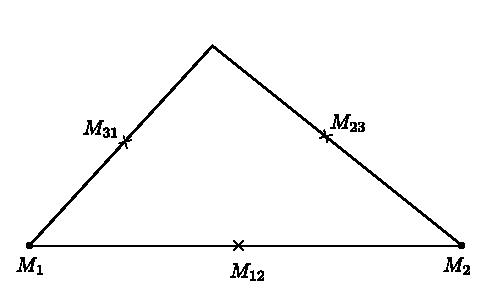
\includegraphics{vol65-figures/fig65-7.1.eps}}
  \caption{}\label{c2:fig7.1}
\end{figure}


Let\pageoriginale $v$ be a function defined on $T$. We define $v_i$ and $v_{jk}$ by  
$$
v_i = v(M_i), v_{jk} = v(M_{jk}).
$$
Then we have the following formulae

\begin{align*}
\int_T uv dx & = \frac{M (T)} {12} \{ (u_1 + u_2) (v_1 +v_2) + (u_2 +
  u_3) (v_2 + v_3)\\ 
  &\hspace{3cm} + (u_3 + u_1) (v_3 + v_1)\} \, \forall  u, v
  \in P_1 , \tag{7.1}\label{c2:eq7.1}
\end{align*}
\begin{equation*}
 \begin{cases}
|\nabla_v|^2 = \frac{1}{4M (T)^2} \{ |\overrightarrow {M_2
  M_3}|^2 v^2_1 + |\overrightarrow{M_3 M_1}|^2 v_2^2 +
|\overrightarrow{M_1 M_2}|^2 v^2_3\\ 
\hspace{5cm}+ \overrightarrow{2 M_2 M_3} \cdot
\overrightarrow{M_3 M_1} v_1 v_2  \\ 
+ \overrightarrow{2M_1 M_2} \cdot \overrightarrow{M_2M_3} v_3v_1 +
\overrightarrow{2M_3M_1} \cdot \overrightarrow{M_1M_2} v_2 v_3\} ,\\ 
\, \forall  v \in P_1, 
\end{cases}\tag{7.2}\label{c2:eq7.2}
\end{equation*}
{\fontsize{10}{12}\selectfont
\begin{equation*}
 \begin{cases}
\int_T |v|^2 dx\\ 
= \frac{M (T)}{3} \{ \frac{1}{10} (v^2_1 + v_2^2 +
v_3^2) + \frac{8}{15} (v_{22}^2 + v^2_{23} +v_{31}^2) - \frac{1}{30}
(v_1 v_2 + v_2 v_3 + v_3 v_1)  \\ 
 + \frac{8}{15} (v_{12} v_{23} + v_{23} v_{31} + v_{31} v_{12}) -
\frac{2}{15} (v_1 v_{23} + v_2 v_{31} + v_3 v_{12})\} , \, \forall 
v \in P_2, \tag{7.3}\label{c2:eq7.3} 
\end{cases}
\end{equation*}}
\begin{equation*}
 \begin{cases}
   \int_T |\nabla v|^2 dx = \frac {1} {12 M (T)} \{ |v_1
   \overrightarrow { M_2 M_3} - v_2\overrightarrow{M_3 M_1} + v_3
   \overrightarrow{M_1 M_2}\\ 
   \hspace{5cm}+ 2 (v_{12} + v_{23} - v_{31})
   \overrightarrow {M_3M_1}|^2  \\ 
    + |v_1 \overrightarrow{M_2 M_3} + v_2 \overrightarrow{M_3 M_1} -
   v_3 \overrightarrow {M_1M_2} + 2 (v_{23} + v_{13} - v_{12})
   \overrightarrow {M_1 M_2} |^2 +\\ 
    + |-v_1 \overrightarrow{M_2 M_3} + v_2 \overrightarrow{M_3 M_1} +
   v_3 \overrightarrow {M_1 M_2} + 2 (v_{31} + v_{12} - v_{23})\\
   \hspace{6.5cm}\overrightarrow {M_2 M_3} |^2\} \, \forall  v \in P_2.\}
   \tag{7.4}\label{c2:eq7.4}
\end{cases}
\end{equation*}\pageoriginale 

The above formulae may be useful to express the approximations of the
problems of this chapter, in a from suitable for computations. 
